% VLDB template version of 2020-08-03 enhances the ACM template, version 1.7.0:
% https://www.acm.org/publications/proceedings-template
% The ACM Latex guide provides further information about the ACM template

\documentclass[sigconf, nonacm]{acmart}

\usepackage{booktabs}

\usepackage{algorithm}
\usepackage{algorithmic}

\usepackage{subcaption}
\usepackage{listings}
\lstset{literate=%
    {Ö}{{\"O}}1
    {Ä}{{\"A}}1
    {Ü}{{\"U}}1
    {ß}{{\ss}}1
    {ü}{{\"u}}1
    {ä}{{\"a}}1
    {ö}{{\"o}}1
    {~}{{\textasciitilde}}1
}

\lstset{
    basicstyle=\ttfamily,
    %frame=single,
    breaklines=true,
    breakatwhitespace=true,
}

\AtBeginDocument{%
  \providecommand\BibTeX{{%
    Bib\TeX}}}

%% The following content must be adapted for the final version
% paper-specific
\newcommand\vldbdoi{XX.XX/XXX.XX}
\newcommand\vldbpages{XXX-XXX}
% issue-specific
\newcommand\vldbvolume{14}
\newcommand\vldbissue{1}
\newcommand\vldbyear{2020}
% should be fine as it is
\newcommand\vldbauthors{\authors}
\newcommand\vldbtitle{\shorttitle} 
% leave empty if no availability url should be set
\newcommand\vldbavailabilityurl{URL_TO_YOUR_ARTIFACTS}
% whether page numbers should be shown or not, use 'plain' for review versions, 'empty' for camera ready
\newcommand\vldbpagestyle{plain} 

\begin{document}
\title{Excel Shrink: An Open-Source Tool for Reducing File Bloat in Excel Spreadsheets}

%%
%% The "author" command and its associated commands are used to define the authors and their affiliations.
\author{Alexander Aue-Johr}
\email{alexander.aue@thuenen.de}
\orcid{0009-0001-8683-3630}
\affiliation{%
  \institution{Thünen Institute for Rural Areas}
  \city{Brunswick}
  \country{Germany}
}

\author{Hardy Pundt}
\email{hpundt@hs-harz.de}
\orcid{https://orcid.org/0000-0001-6985-5929}
\affiliation{%
  \institution{Harz University of Applied Sciences}
  \city{Wernigerode}
  \country{Germany}
}

%%
%% The abstract is a short summary of the work to be presented in the
%% article.
\begin{abstract}
  Excel files are widely used for data exchange across various domains. However, as spreadsheets grow in complexity, they often suffer from file bloat, leading to significant challenges in file size and performance management. We investigated Excel files from the German Federal Statistical Office (Destatis) and observed extremely long load times in Microsoft Excel and crashes due to out-of-memory exceptions in software packages used for reading Excel files. Our analysis revealed that these files contain format definitions invisible to the user, which occupy orders of magnitude more storage space than the actual data.

  While some existing tools attempt to address this issue, they often fail to fully resolve the problem or introduce new issues, such as altering the visual appearance of spreadsheets. In this paper, we present a comprehensive analysis of the root causes of Excel file bloat, documenting issues that have been partially addressed by existing tools but remained undocumented, and uncovering additional issues not resolved by these tools. We also analyze why these tools impact the visual integrity of Excel files.
  

  We developed an open-source tool, Excel Shrink Analyser, welches wir benutzt haben um herrauszufinden, wodurch die der file bloat in exceldateien entsteht. Auf Grundlage der Ergebnisse wussten wir nach welchen Dateiinhalten wir suchen mussten und haben uns das ziel gesetzt die ein performanceoptimiertes commandozeilenprogramm zu entwickeln, welches dieselben bereinigungen vornimmt aber dabei deutlich schneller ist um so eine geschwindigkeit zu erreichen, die es sinnvoll macht die datei immer erst mit excel Shrink zu bereinigen, bevor man sie mit dem gewünschten Programm oder der gewünschten bibliothekten öffnet, weil die ausführungszeit durch das vorherige bereinigen und das anschließende öffnen durch die bibliothek oder programm schneller ist, als die Excel datei direkt mit dem gewünschten programm oder der gewünschten bibliothek zu öffnen. Wir konnten erfolgreich das programm so optimieren, dass es Excel Dateien öffnen, bereinigen und wieder speichern kann und dabei doppelt so schnell ist, als Microsoft excel es schafft die datei zu öffnen.
  
  Optional: Wir haben auch its graphical user interface counterpart, Excel Shrink UI entwickelt, which effectively address both the known and previously unresolved root causes of Excel file bloat without compromising the visual appearance of the spreadsheets. Excel Shrink UI enables users to optimize their Excel files without the need for programming knowledge or command-line tools. To evaluate our tools, we downloaded all Excel files from Destatis and optimized them using Excel Shrink. Our results show that our tools can reduce file sizes by up to 99.99\% without affecting the visual integrity of the files.
\end{abstract}

\maketitle

%%% do not modify the following VLDB block %%
%%% VLDB block start %%%
\pagestyle{\vldbpagestyle}
\begingroup\small\noindent\raggedright\textbf{PVLDB Reference Format:}\\
\vldbauthors. \vldbtitle. PVLDB, \vldbvolume(\vldbissue): \vldbpages, \vldbyear.\\
\href{https://doi.org/\vldbdoi}{doi:\vldbdoi}
\endgroup
\begingroup
\renewcommand\thefootnote{}\footnote{\noindent
This work is licensed under the Creative Commons BY-NC-ND 4.0 International License. Visit \url{https://creativecommons.org/licenses/by-nc-nd/4.0/} to view a copy of this license. For any use beyond those covered by this license, obtain permission by emailing \href{mailto:info@vldb.org}{info@vldb.org}. Copyright is held by the owner/author(s). Publication rights licensed to the VLDB Endowment. \\
\raggedright Proceedings of the VLDB Endowment, Vol. \vldbvolume, No. \vldbissue\ %
ISSN 2150-8097. \\
\href{https://doi.org/\vldbdoi}{doi:\vldbdoi} \\
}\addtocounter{footnote}{-1}\endgroup
%%% VLDB block end %%%

%%% do not modify the following VLDB block %%
%%% VLDB block start %%%
\ifdefempty{\vldbavailabilityurl}{}{
\vspace{.3cm}
\begingroup\small\noindent\raggedright\textbf{PVLDB Artifact Availability:}\\
The source code, data, and/or other artifacts have been made available at \url{\vldbavailabilityurl}.
\endgroup
}
%%% VLDB block end %%%

\section{Introduction}

Excel spreadsheets are integral to a wide range of domains—including finance, statistics, business, and research—due to their flexibility in managing tabular data, executing complex calculations, automating workflows via macros, and visualizing information using charts and graphs \cite{panko1998we, Rahman2021NOAH, userExperienceSpreadsheets2022}. However, as these spreadsheets grow in size and complexity, they often suffer from performance bottlenecks, file bloat, and increased processing delays \cite{swidan2016improving, tang2023efficient, antiFreezeBendre2019sigmod, Bendre2015DataSpread}.

Unlike simpler formats such as CSV, Excel files leverage the Office Open XML architecture introduced in Excel 2007 \cite{ecma376-5th2021}. Under this format, data, formatting, shared strings, and other metadata are stored as a collection of XML files, all compressed into a single ZIP archive. This design supports advanced features, such as separating data from formatting—e.g., centralizing repeated strings in a shared string table \cite{microsoft2024sharedstring}, or storing fonts, cell styles, and colors in dedicated XML files. While this architecture enables functionality beyond what simpler formats provide, it also creates opportunities for hidden inefficiencies to emerge.

Die Herrausforderungen mit dem filebloat in excel Dateien sind:
Excel benötigt einige Zeit um diese Dateien zu öffnen.
In excel veringert sich die anzeigegeschwindigkeit auf bloated arbeitsblättern, vor allem beim scrollen.
Bilbiotheken, die erlauben excel dateien auszulesen, und in python, R oder anderen Sprachen zu verarbeiten, öffnen diese Dateien ebenso sehr langsam und manchmal stürzen sie sogar durch den file bloat ab, da sie gängige  XMl parsing technologien wie einen dom parser nutzen, diese auch mit gewöhnlichen Excel Dateien gut klar kommen, da dort die xml dateien der arbeitsblätter klein genug dafür sind, aber genau diese technologien wie ein domparser können mit diesen arbeitsblättern die an filebloat leiden nicht umgehen, sie sind nicht für enorm große daten optimiert und stürzen infolgedessen durch outofmemory exceptions ab.
Manche Programme wie Texteditoren wie IntelliJ verweigern sogar die vollständige  anzeige dieser dateien und zeigen nur den Anfang der Datei.
Andere Texteditoren wie visual studio code, öffnen diese Dateien zwar in machen fällen, manchmal aber erst nachdem man den Prompt zum keep waiting oder abbrechen ein bis mehrere male geklickt hat oder es stürzt beim versuch die arbeitsblatt xml Datei zu öffnen ab.
Wenn visual studio code doch in der lage ist, eine sehr arbeitsblatt xml Datei zu öffnen, dann erlaubt es aber keine gängigen funktionen die das formatieren des XML codes.
Ausgerechnet dies wäre aber hilfreich, om die XML struktur anzusehen um herrauszufinden, wo der bloat in der Datei liegt um ihn ggf manuell zu entfernen.  

Introduction: Excel spreadsheets are ubiquitous in business, science, and government for managing data, but as they grow in complexity they often suffer from severe “file bloat.” In practice, bloated Excel files can swell to hundreds of megabytes and become painfully slow or even impossible to process. Real-world cases have reported extremely long load times in Microsoft Excel and out-of-memory crashes in Python/R libraries when opening such files​
FILE-VODJZZXWMSJQYRIMK3LKRJ
. The culprit is typically an accumulation of redundant or invisible content in the workbook’s XML: format definitions and placeholders that are not visible to the user yet occupy orders of magnitude more space than the actual cell data​
FILE-VODJZZXWMSJQYRIMK3LKRJ
. Practitioners have long noticed that clearing unused formatting or trimming the “used” range of a worksheet can dramatically shrink file size​
FILE-VODJZZXWMSJQYRIMK3LKRJ
, indicating that much of the bloated data stems from unnecessary metadata. However, there is a lack of peer-reviewed studies quantifying the causes of Excel file bloat – most guidance on this problem comes from anecdotal reports rather than formal analysis​
FILE-VODJZZXWMSJQYRIMK3LKRJ
. This gap motivates a systematic investigation into why Excel files bloat and how we can efficiently remediate it.Modern Excel files use the Office Open XML (OOXML) format [18], which means an .xlsx workbook is essentially a ZIP archive containing multiple XML files for data, styles, and other information​
FILE-VODJZZXWMSJQYRIMK3LKRJ
. For example, cell contents and formulas reside in per-sheet XML files, a global sharedStrings.xml holds all repeated text, and styles.xml defines cell formatting (fonts, colors, etc.). This design—introduced in Excel 2007 to separate data from presentation—enables advanced features like centralizing duplicate strings in a shared table to reduce file size​
FILE-VODJZZXWMSJQYRIMK3LKRJ
. Ironically, the same architecture also creates opportunities for hidden inefficiencies: the XML parts can grow with superfluous entries (e.g. thousands of empty cells with formatting) that inflate the file without affecting the visible content​
FILE-VODJZZXWMSJQYRIMK3LKRJ
. In other words, the structured OOXML format makes it possible for a workbook to carry a large amount of baggage (in the form of XML markup) that the user never sees, leading to bloated files and degraded performance.Parsing and processing these bloated XML-based spreadsheets efficiently is challenging. Traditional XML parsing techniques like DOM and SAX exhibit significant inefficiencies on large Excel files. A DOM parser, which builds an in-memory tree of the entire XML, can easily exhaust memory on multi-hundred-thousand-row sheets, whereas a streaming SAX parser avoids high memory usage but suffers high CPU overhead from handling a flood of callback events​
FILE-VODJZZXWMSJQYRIMK3LKRJ
. In practice, this means that libraries using DOM (for example, the R readxl package) often run out of memory or slow down drastically on oversized .xlsx files, while pure SAX-based solutions spend excessive time processing element-by-element events​
FILE-VODJZZXWMSJQYRIMK3LKRJ
​
FILE-VODJZZXWMSJQYRIMK3LKRJ
. Hybrid approaches attempt to strike a balance: for instance, the R openxlsx library mixes SAX parsing with regex-driven extraction of important content, yet even such optimizations can remain slow and memory-intensive in worst-case scenarios​
FILE-VODJZZXWMSJQYRIMK3LKRJ
. On the other hand, DOM-heavy tools may achieve faster runtime on small files but at the cost of extremely high memory consumption on large ones (in some cases using >10× the size of the uncompressed data)​
FILE-VODJZZXWMSJQYRIMK3LKRJ
. These issues are well documented in recent research – for example, Henze et al. [20] report that the readxl DOM parser can use 10× memory, and introduced a specialized streaming parser (SheetReader) that prunes extraneous formatting on the fly and parallelizes parsing, achieving 40× lower memory usage and 3× faster load times compared to standard libraries​
FILE-VODJZZXWMSJQYRIMK3LKRJ
​
FILE-VODJZZXWMSJQYRIMK3LKRJ
. Overall, a clear trade-off has emerged: DOM-based methods are simpler to implement but incur heavy memory overhead, whereas SAX-based methods are more memory-efficient but CPU-intensive; domain-specific techniques (like selectively skipping over style XML or using custom stream processors) can sometimes hit a sweet spot in between​
FILE-VODJZZXWMSJQYRIMK3LKRJ
. Yet, despite these advances, even today no mainstream spreadsheet software handles gigantic Excel files gracefully out-of-the-box, especially when bloated with unnecessary XML data.In this paper, we explore a novel approach to efficiently handle bloated Excel files by operating directly on the raw XML byte stream with the help of regular expressions and a state machine. The idea is to pre-process the spreadsheet file at the text level – treating the sheet XML as plaintext – to quickly eliminate bloating content (such as thousands of blank formatted cells or redundant style definitions) before loading the data into Excel or an analysis tool. This byte-stream processing leverages the raw speed of regex pattern matching while a custom state machine provides just enough structural awareness to avoid damaging the XML format. In essence, we scan through the workbook’s XML text and apply a series of targeted regex replacements to remove or compress bloat, but we do so within a controlled framework that knows which section of the file is being processed​
FILE-VODJZZXWMSJQYRIMK3LKRJ
. For example, the state machine can distinguish between being inside the <sheetData> (cell data) section versus in metadata sections, and trigger different regex rules accordingly​
FILE-VODJZZXWMSJQYRIMK3LKRJ
. This contextual control is crucial because applying regex blindly on XML can be dangerous – a careless pattern might “overmatch” and inadvertently remove legitimate content or break the XML structure. By maintaining a small buffer of context (such as which row or column section is active, and references to shared strings and styles)​
FILE-VODJZZXWMSJQYRIMK3LKRJ
, our method ensures that each regex substitution occurs only in the appropriate scope. Thus, the state machine mitigates the usual drawbacks of regex on hierarchical data, effectively combining the performance of text-stream processing with the safety of structure-aware parsing. We hypothesize that this approach can dramatically reduce file bloat with minimal overhead, making it feasible to clean an .xlsx file as a preprocessing step in less time than it would take Excel or a library to load the bloated file directly.To guide our study, we pose the following research questions: (RQ1) Can a regex-driven, state-machine–guided parser overcome the typical limitations of regular expressions in processing structured XML data (e.g., prevent overmatching and preserve XML validity)? (RQ2) Does precleaning bloated Excel files with such a method significantly improve overall loading time (i.e., cleaning + loading) compared to loading the original file directly in Excel or popular Python/R libraries? (RQ3) Are the root causes of Excel file bloat already well-understood and documented in existing research, or is further empirical analysis needed to fully identify and quantify these causes? The third question is motivated by the aforementioned lack of formal literature on Excel bloat​
FILE-VODJZZXWMSJQYRIMK3LKRJ
 – while various blog posts and support articles enumerate possible causes (extra formatting, unused styles, etc.), we aim to determine whether these cover all major contributors or if additional, undocumented factors emerge from a systematic investigation. By addressing these questions, our work seeks to both improve practical handling of large Excel files and deepen the scientific understanding of Excel bloat, ultimately enabling more efficient data workflows in spreadsheet-based analytics.


\section{Background}
 

\subsection{Excel’s Internal Storage Mechanisms and Resulting Inefficiencies}

The ZIP-based compression of XML data efficiently reduces file size by exploiting repetitive tags and structures \cite{deutsch1996deflate}. Yet, this approach can mask significant redundancies. Over time, spreadsheets can accumulate unnecessary formatting or metadata: for instance, entire rows or columns may be formatted even though only a subset of cells contain data \cite{cunha2012smellsheet, abreu2014faultysheet}. Similarly, duplicating a sheet transfers all formatting, styles, and hidden elements, even when most of them are not needed \cite{Mack2018Scalability}. Such practices lead to inflated files, slower load times, and degraded performance \cite{Mack2018Scalability, Rahman2020Benchmarking}—issues that become especially problematic in large-scale enterprise environments or when dealing with extensive datasets, such as those provided by the German Federal Statistical Office (Destatis).

\section{Related Work}
\label{sec:related-work}

A substantial body of research in top-tier venues (VLDB, SIGMOD, ICDE) has explored techniques to \emph{improve performance} on large or complex workbooks. There have also been several efforts to reduce \emph{Excel file size}, with various online resources discussing this topic. We briefly review key findings below, focusing on (i) methods for minimizing file size, (ii) approaches to accelerating computation and user interactions for large spreadsheets, (iii) optimizations for parsing the XML-based \texttt{.xlsx} format, and (iv) highlights of Aditya Parameswaran’s contributions in bridging spreadsheet and database technologies.

\textbf{Minimizing Excel File Size and Bloat.}
Microsoft’s transition from the binary \texttt{.xls} format to \texttt{.xlsx} (Office Open XML) introduced compression and a shared string table to reduce repeated data \cite{ecma2007openxml,Microsoft2007OpenXML}. Further reduction is achieved in the \texttt{.xlsb} (binary) format, which stores data in a compact binary container at the cost of certain compatibility constraints \cite{MicrosoftXLSB,Mack2018Scalability}.

However, there is a lack of peer-reviewed studies specifically quantifying how “bloat” (whitespace values, invisible formatting, rows and column definitions outside of the visible content) affects Excel file size. Instead, most advice on the subject comes from practitioners sharing their experiences. For example, Microsoft’s support article on cleaning excess cell formatting provides practical tips for reducing file size and improving performance \cite{microsoft_support}. Additionally, discussions on forums such as MrExcel illustrate that users have long noticed dramatic size reductions after clearing unused formatting or trimming the “used range” \cite{excelforum}. Popular Excel blogs from UpSlide \cite{upslide_blog} and The Bricks \cite{thebricks_blog}  further detail these methods based on accumulated user experience rather than formal experimentation.

Several proprietary tools have been developed to address Excel bloat automatically. Notable examples include UpSlide’s Automation Software, which offers a one-click “Smart Clean” feature \cite{upslide_blog}; NXPowerLite Desktop \cite{neuxpower2024nxpowerlite}; Sobolsoft’s Excel File Size Reduce Software \cite{sobolsoft}; and online services such as WeCompress \cite{wecompress}. Other tools, such as Kernel for Excel Repair \cite{kernel_excel}, have also been mentioned in user communities for their file compression capabilities.

Excel has also developed two tools to assist users. One such tool is \textbf{Excel Inquire}, an add-in introduced with Excel 2013 that provides a range of auditing features—including Workbook Analysis, Relationship Diagrams, and the Clean Excess Cell Formatting command. O'Beirne discusses this in the proceedings of the EuSpRIG 2013 Conference on “Spreadsheet Risk Management” \cite{obeirne2013}, noting that the \textit{Clean Excess Cell Formatting} command removes excess formatting but does not indicate beforehand what will be cleared, nor does it report afterwards what was removed.

More recently, Microsoft introduced the \textbf{Excel Performance Tab}, a built-in feature designed to monitor workbook performance by identifying inefficiencies and offering cleaning recommendations. However, the Performance Tab has received negative user feedback; several users report that its forced “Check Performance” pop-up and the associated reformatting remove intentional formatting and disrupt workflows \cite{mrexcel2024check,microsoft_cleanup} and also Excel users report theat their pixel art is deleted \cite{mrexcel2024check} while the Microsoft Support Seite even mentions a warning that pixel art will be removed by the tool \cite{microsoft_cleanup}.

In contrast, our paper provides a comprehensive scientific analysis of the root causes of Excel file bloat in XML-based workbooks. To address this gap, we introduce \textit{Excel Shrink}---a free, open-source command-line tool designed for automation pipelines. Unlike proprietary tools that are only accessible through a graphical user interface and sometimes remove too many elements (thereby altering the visual appearance) or too few (leaving the file size large), Excel Shrink selectively reduces file size by eliminating only those elements that do not affect the workbook’s visual integrity.

\textbf{Performance in Handling Large Spreadsheets.}
Rahman et al.~\cite{Rahman2020Benchmarking} conducted a comprehensive study comparing Excel, LibreOffice Calc, and Google Sheets on sizable datasets. They revealed that despite nominal row limits of one million, Excel’s GUI would often freeze with mere tens of thousands of rows or extended formula usage. Similar findings appear in other bench\-marking efforts 
\cite{Rahman2021NOAH}, 
highlighting the lack of query-planning or indexing in typical spreadsheet software. Addressing this, “DataSpread”~\cite{Bendre2015DataSpread} (VLDB 2015) and “Hillview”~\cite{Budiu2019Hillview} (PVLDB 2019) offload data management to database engines or distributed clusters, respectively, while retaining a spreadsheet-like interface. These architectures stretch the notion of a “spreadsheet” to hundreds of millions (or billions) of rows by introducing parallelization, indexing structures, or incremental computation. In a different line of work, Bendre et al.~\cite{Bendre2019AntiFreeze} proposed an \emph{anti-freeze} model for formula recalculation, allowing asynchronous updates so the user interface does not lock while large spreadsheets recompute.

\textbf{Efficient Excel XML Processing.}
As modern Excel files (\texttt{.xlsx}) are essentially XML (SpreadsheetML) within a ZIP container, \emph{parsing} can become a bottleneck for large sheets. Classical DOM-based XML parsing can exhaust memory on multi-hundred-thousand-row spreadsheets, whereas SAX-based streaming, though more memory-friendly, suffers from high CPU overhead through numerous event callbacks 
\cite{Henze2022SheetReader}. 
A hybrid parser that combines DOM and SAX parsing, along with regular expressions for extracting the relevant file contents (e.g.\ \texttt{openxlsx} in R), can still be slow and memory-intensive under worst-case scenarios. By contrast, parsers relying exclusively on DOM parsing (e.g.\ \texttt{readxl} in R) may achieve faster runtime performance but often at the cost of higher memory usage. For instance, the memory consumption of \texttt{readxl} can exceed ten times the size of the uncompressed worksheet \cite{Henze2022SheetReader}. 
To address this, Henze et al.~\cite{Henze2022SheetReader} introduced \emph{SheetReader}, a specialized streaming parser that integrates decompression and XML scanning, prunes unneeded formatting metadata early, and parallelizes chunk-level parsing. This yields dramatically lower memory footprints (often $40\times$ less) and faster loads ($3\times$ or more) compared to standard libraries.

\textbf{Comparisons of Parsing Approaches and Tools.}
These studies collectively show a trade-off between \emph{DOM-based} simplicity (at the cost of high memory usage) and fully \emph{SAX-based} pipelines (often incurring higher CPU overhead). Hybrid or domain-specific solutions—like regex-based extraction or streaming chunk processors that skip unneeded style markup—strike a middle ground 
\cite{openxlsx, Henze2022SheetReader}. 
Meanwhile, broad tool evaluations (Microsoft Excel vs.\ Google Sheets vs.\ LibreOffice Calc) confirm that no mainstream spreadsheet program handles truly large data sets efficiently out of the box 
\cite{Rahman2020Benchmarking}.

\textbf{Parameswaran’s Contributions: Bridging Spreadsheets and Databases.}
Aditya Parameswaran and collaborators have extensively researched integrating spreadsheets with database backends to achieve both usability and scalability 
\cite{Bendre2015DataSpread, Bendre2018PDM}. 
\emph{DataSpread} preserves the familiar Excel-like interface while relying on a relational DBMS for storage and large-scale computations, enabling interactive performance even at billions of cells. This approach can be seen as bypassing Excel’s internal storage and recalculation limits by adopting database features (indexing, query optimization, concurrency control). In related work on “anti-freeze” recalculation, Parameswaran’s group explored asynchronous formula evaluation with incremental updates, preventing interface lock-ups for large or complex dependency graphs 
\cite{Bendre2019AntiFreeze}. 
Additionally, they highlight practical tactics like saving spreadsheets as binary (\texttt{.xlsb}) instead of \texttt{.xlsx} to mitigate bloat, limiting volatile formulas (e.g.\ \texttt{OFFSET}), and offloading heavy operations to databases where possible 
\cite{Mack2018Scalability}. 
All these strategies offer evidence that a combination of advanced parsing, background recalculation, and robust data management techniques can significantly enhance performance for real-world Excel workloads.

\paragraph{Summary.}
From straightforward file-format optimizations (\texttt{.xlsb} compression) to \emph{architectural} overhauls (DataSpread, Budiu2019Hillview) and specialized parsers (SheetReader), the research consensus is that Excel’s native engine and file format alone do not scale gracefully. Modern solutions increasingly combine streaming-based XML handling, database or distributed architectures, and asynchronous computation to push spreadsheet interactivity far beyond Excel’s historical limits. These insights strongly motivate the need for further improvements in \texttt{.xlsx} bloat reduction and high-performance parsing directly addressed by our proposed approach in this paper.


\section{Introduction}
\label{sec:introduction}




\noindent
\textbf{Research Challenge:} Standard XML-based solutions---such as DOM or SAX parsers---become prohibitively slow or run out of memory on these bloated spreadsheets. Our central question is:
\emph{``Can we remove spreadsheet bloat without fully decoding each XML file, while still preserving the user’s visible layout?’’}
\\

\noindent
\textbf{Contributions:}
\begin{itemize}
    \item We identify key obstacles to high-performance Excel de-bloating, including hierarchical XML subfiles, hidden formatting, and partial sheets with large row or column definitions.
    \item We propose a \emph{byte-stream-based}, \emph{multiprocessing} approach that leverages dynamic regular expressions to remove invisible content \emph{in flight}, guided by minimal reading of critical metadata such as \texttt{styles.xml} or \texttt{sharedStrings.xml}.
    \item We show that this method can outperform not only typical DOM or SAX-based solutions but even Excel’s built-in tools like the Inquire Add-in or \emph{Check Performance}---in many cases completing the cleaning \emph{faster} than the time Excel needs just to open the file.
    \item We evaluate on over 1,200 real-world Excel files from the German Federal Statistical Office, achieving up to 99.99\% reduction in file size with intact layout and style.
\end{itemize}

Our results have broad implications for data management systems that face large, unwieldy XML-based archives. By highlighting and tackling the difficulties of streaming modifications on nested, compressed data, we aim to enrich the conversation about advanced transformations for file-based data exchange.

\section{Background}
\label{sec:background}




%\begin{algorithm}
%  \caption{Extract Row Styles from XML Buffer}
%  \label{alg:extract_row_styles}
%  \begin{algorithmic}
%
%    \STATE \textbf{Input:} 
%    \STATE \quad \texttt{Buf} $\leftarrow$ Byte buffer containing XML row data
%    \STATE \quad \texttt{Sty} $\leftarrow$ Extracted style definitions
%    \vspace{0.2cm}
%
%    \STATE \textbf{Initialize:}
%    \STATE \quad \texttt{RowStylesDict} $\leftarrow$ Empty dictionary
%    \STATE \quad \texttt{RowPattern} $\leftarrow$ Regex pattern to match \texttt{"<row ...>"} elements
%    \vspace{0.2cm}
%
%    \STATE \textbf{Search for Row Elements}
%    \FOR{each match \texttt{M} in \texttt{RowPattern} applied to \texttt{Buf}}
%        \STATE \texttt{RowTag} $\leftarrow$ Extracted row element
%        \STATE \texttt{AttrPairs} $\leftarrow$ Extract all attributes as key-value pairs
%        \STATE \texttt{Attrs} $\leftarrow$ Convert attributes to dictionary
%        \vspace{0.2cm}
%
%        \STATE \textbf{Process Row Style}
%        \IF{\texttt{"s"} and \texttt{"r"} exist in \texttt{Attrs}}
%            \STATE \texttt{RowStyleID} $\leftarrow$ Convert \texttt{"s"} attribute to integer
%            \STATE \texttt{RowID} $\leftarrow$ Convert \texttt{"r"} attribute to integer
%            \STATE \textbf{Try:}
%                \STATE \quad \texttt{RowXF} $\leftarrow$ Retrieve \texttt{RowStyleID} from \texttt{Sty.cellXfs}
%                \STATE \quad \texttt{RowStylesDict[RowID]} $\leftarrow$ \texttt{RowXF}
%            \STATE \textbf{Except:}
%                \STATE \quad Skip row if style index is invalid
%        \ENDIF
%    \ENDFOR
%    \vspace{0.2cm}
%
%    \STATE \textbf{Output:} \texttt{RowStylesDict}, mapping row IDs to extracted styles
%
%  \end{algorithmic}
%\end{algorithm}


%\begin{algorithm}
%  \caption{Extract Row Styles from XML Buffer}
%  \label{alg:extract_row_styles}
%  \begin{algorithmic}
%
%    \STATE \textbf{Input:} 
%    \STATE \quad \texttt{Buf} $\leftarrow$ Byte buffer containing XML row data
%    \STATE \quad \texttt{Sty} $\leftarrow$ Extracted style definitions
%    \vspace{0.2cm}
%
%    \STATE \textbf{Initialize:}
%    \STATE \quad \texttt{RowStylesDict} $\leftarrow$ Empty dictionary
%    \STATE \quad \texttt{RowPattern} $\leftarrow$ Regex pattern to match \texttt{"<row ...>"} elements
%    \vspace{0.2cm}
%
%    \STATE \textbf{Search for Row Elements}
%    \FOR{each match \texttt{M} in \texttt{RowPattern} applied to \texttt{Buf}}
%        \STATE \texttt{RowTag} $\leftarrow$ Extracted row element
%        \STATE \texttt{AttrPairs} $\leftarrow$ Extract all attributes as key-value pairs
%        \STATE \texttt{Attrs} $\leftarrow$ Convert attributes to dictionary
%        \vspace{0.2cm}
%
%        \STATE \textbf{Process Row Style}
%        \IF{\texttt{"s"} and \texttt{"r"} exist in \texttt{Attrs}}
%            \STATE \texttt{RowStyleID} $\leftarrow$ Convert \texttt{"s"} attribute to integer
%            \STATE \texttt{RowID} $\leftarrow$ Convert \texttt{"r"} attribute to integer
%            \STATE \textbf{Try:}
%                \STATE \quad \texttt{RowXF} $\leftarrow$ Retrieve \texttt{RowStyleID} from \texttt{Sty.cellXfs}
%                \STATE \quad \texttt{RowStylesDict[RowID]} $\leftarrow$ \texttt{RowXF}
%            \STATE \textbf{Except:}
%                \STATE \quad Skip row if style index is invalid
%        \ENDIF
%    \ENDFOR
%    \vspace{0.2cm}
%
%    \STATE \textbf{Output:} \texttt{RowStylesDict}, mapping
%
% 
%  \end{algorithmic}
%\end{algorithm}








\section{Methodology4}
\label{sec:methodology4}

Our methodology evolved from an initial DOM-based prototype, the \emph{Excel Shrink Analyzer}, which helped us investigate and understand the primary causes of file bloat in large Excel files. This analysis revealed that excessive file sizes primarily resulted from hidden rows, empty but styled cells, bloated shared strings, and unnecessary columns.

Because we encountered frequent memory limitations and poor scalability using XML-based approaches, we shifted to a \emph{stream-based approach}. This change was motivated by the insight that an efficient processing model could be implemented using \emph{regex-based chunk processing} on the raw bytestream. To achieve this, we maintained a small buffer tracking essential context such as row/column states and style references.

Constructing effective regular expressions required more than a simple pattern, given the hierarchical nature of Excel’s XML structure. Consequently, we developed a pipeline of multiple regex stages, each designed to target a specific inefficiency in spreadsheet data:

1. Identify whitespace-only shared strings and remove their referencing cells if they do not have a visible style.
2. Delete purely empty cells lacking any borders or fill styles.
3. Truncate rows and columns that fall outside the bounding box of the visible data region.
4. Prune unnecessary column definitions, ensuring the final column range still extends to \texttt{XFD} (the maximum column index in Excel) to preserve layout.

This systematic approach enables efficient, scalable file-size reduction without requiring large in-memory representations, thereby significantly improving both performance and storage efficiency.

\subsection{Multithreading for Performance}
To further increase parsing speed, we use multithreading. In this approach, each XML file within the ZIP archive is processed by its own thread. Because each thread splits the large \texttt{worksheetX.xml} files into smaller chunks and processes these chunks incrementally, only a negligible amount of memory is used per thread. This setup represents a significant improvement over our previous DOM-based approach, where a single thread attempted to process all worksheets consecutively. The DOM-based method consistently consumed nearly 100\% of the available memory on our test machine, which prevented any realistic automation. By contrast, our new approach effectively reduces overall computation time and allows the files to be processed more quickly.

\begin{algorithm}[ht]
  \caption{Processing and Cleaning Excel Files in Place}
  \label{alg:process_xlsx_in_place2}
  \begin{algorithmic}

    \STATE \textbf{Input:} 
    \STATE \quad \texttt{InP} $\leftarrow$ Excel file path
    \STATE \quad \texttt{OutP} $\leftarrow$ Output path
    \vspace{0.2cm}
    
    \STATE \texttt{InArc} $\leftarrow$ Open the ZIP archive \texttt{InP} for reading
    \STATE \texttt{OutArc} $\leftarrow$ Create a new ZIP archive for writing
    \STATE \texttt{ShStr} $\leftarrow$ Extract shared strings from \texttt{sharedStrings.xml}
    \STATE \texttt{Sty} $\leftarrow$ Extract styles from \texttt{styles.xml}
    \STATE \texttt{SF} $\leftarrow$ List of all sheet XML files in \texttt{InArc}
    \STATE \texttt{NSF} $\leftarrow$ List of non-sheet files in \texttt{InArc}    
    \vspace{0.2cm}

    \STATE \texttt{wvp} $\leftarrow$ dynamically create a pattern based on \texttt{ShStr} to identify whitespace-only cell values
    \STATE \texttt{icp} $\leftarrow$ dynamically create a pattern based on \texttt{Sty} to identify cells that are invisible
    \STATE \texttt{sdcp} $\leftarrow$ dynamically create a pattern based on \texttt{Sty} to identify cells whose styles depend on row/column styles 
    \vspace{0.2cm}
    \STATE \FOR{each sheet file \texttt{sf} in \texttt{SF} \textbf{in parallel}}
        \STATE Clean sheet file \texttt{sf} in a stream-based manner using \texttt{wvp}, \texttt{icp}, \texttt{sdcp}, and \texttt{Sty}
        \STATE Write cleaned sheet back to the ZIP archive \texttt{OutArc}
    \ENDFOR

    \STATE \FOR{each non-sheet file \texttt{nsf} in \texttt{NSF}}
        \IF{\texttt{nsf} is \texttt{workbook.xml}}
            \STATE Clean workbook metadata with a DOM-based approach
            \STATE Write cleaned workbook to \texttt{OutArc}
        \ELSE
            \STATE Copy \texttt{nsf} unchanged to \texttt{OutArc}
        \ENDIF
    \ENDFOR

    \STATE \textbf{Output:} Cleaned Excel file

  \end{algorithmic}
\end{algorithm}

\subsection{Methodology (High-Level State-Machine Overview)}

As mentioned above, our new approach employs a state machine that helps manage the complexity of the operations needed to segment the file and apply different regular expressions. The state machine is split into multiple states, each representing a specific file section under processing. Below is an overview of the algorithm:

\begin{algorithm}[ht]
  \caption{Streaming-Based Cleaning of Excel Sheet Data}
  \label{alg:clean_sheet_stream}
  \begin{algorithmic}

    \STATE \textbf{Input:} 
    \STATE \quad \texttt{SheetS} $\leftarrow$ Sheet XML stream
    \vspace{0.2cm}

    \STATE \textbf{Initialize:}
    \STATE \quad \texttt{Buffer} $\leftarrow$ Empty buffer
    \STATE \quad \texttt{Output} $\leftarrow$ Empty buffer
    \STATE \quad \texttt{State} $\leftarrow$ BEFORE\_COLS
    \STATE \quad \texttt{MaxRow} $\leftarrow$ 0
    \STATE \quad \texttt{MaxCol} $\leftarrow$ 0
    \vspace{0.2cm}

    \STATE \textbf{Processing Sheet Stream}
    \WHILE{\texttt{State} $\neq$ END\_OF\_FILE}
        \STATE Read chunk from \texttt{SheetS} into \texttt{Buffer}

        \STATE \IF{\texttt{State} is in BEFORE\_COLS, BEFORE\_SHEET\_DATA \textbf{or} AFTER\_SHEET\_DATA} 
            \IF{Found \texttt{<cols>} or \texttt{<sheetData>}}
                \STATE Store \texttt{Buffer} in \texttt{Output} until last found tag
                \STATE Discard content in \texttt{Buffer} until last found tag
            \ENDIF
            \IF{Found \texttt{<cols>}}
              \STATE \texttt{State} $\leftarrow$ IN\_COLS
            \ELSIF{Found \texttt{<sheetData>}}
                \STATE \texttt{State} $\leftarrow$ IN\_SHEET\_DATA
            \ELSIF{Reached end of file}
                \STATE Store entire \texttt{Buffer} in \texttt{Output} 
                \STATE \texttt{State} $\leftarrow$ END\_OF\_FILE
            \ENDIF
        \ELSIF{\texttt{State} is IN\_COLS}
            \IF{Found \texttt{</cols>} or \texttt{<col/>}}
                \STATE Parse column definitions
                \STATE Store \texttt{Buffer} in \texttt{Output} until last found tag
                \STATE Discard content in \texttt{Buffer} until last found tag
            \ENDIF
            \IF{Found \texttt{</cols>}}
                \STATE \texttt{State} $\leftarrow$ BEFORE\_SHEET\_DATA
            \ENDIF
        \ELSIF{\texttt{State} is IN\_SHEET\_DATA}
            \IF{Found \texttt{</row>}, \texttt{<row .../>} or \texttt{</sheetData>}}
                \STATE Clean \texttt{Buffer} of invisible cells/rows using patterns
                \STATE Store cleaned \texttt{Buffer} in \texttt{Output}
                \STATE Discard content in \texttt{Buffer} until last found tag
                \STATE Extract any remaining cell references to update \texttt{MaxRow} and \texttt{MaxCol}
            \ENDIF
            \IF{Found \texttt{</sheetData>}}
                \STATE \texttt{State} $\leftarrow$ AFTER\_SHEET\_DATA
            \ENDIF
        \ENDIF
    \ENDWHILE
    \vspace{0.2cm}

    \STATE \textbf{Post-Processing}
    \STATE Extract and update \texttt{MaxRow} and \texttt{MaxCol} from merge cells
    \STATE Remove rows exceeding \texttt{MaxRow} from \texttt{sheetData}
    \STATE Merge extraneous columns beyond \texttt{MaxCol}
    \vspace{0.2cm}

    \STATE \textbf{Output:} Cleaned sheet XML

  \end{algorithmic}
\end{algorithm}

We implement our spreadsheet parser as a streaming-based state machine, processing the XML data incrementally to minimize memory consumption and permit early discarding of unnecessary file sections. Both our “consecutive” and “interleaved” parsing approaches, which reduce memory usage, use this same underlying state machine. Below, we focus on how the parser transitions between states (i.e., how each state function decides to proceed), deferring lower-level details of in-state processing until later sections.

\paragraph{States Overview.}
We define six main states in our parser:
\begin{itemize}
  \item \texttt{BEFORE\_COLS}: The parser has not yet encountered the \texttt{<cols>} element. It searches for either \texttt{<cols>} or \texttt{<sheetData>}.
  \item \texttt{IN\_COLS}: The parser found \texttt{<cols>} and is processing column definitions.
  \item \texttt{BEFORE\_SHEET\_DATA}: The parser has finished reading (or did not detect) the \texttt{<cols>} node and is searching for the first \texttt{<sheetData>} element.
  \item \texttt{IN\_SHEET\_DATA}: The parser is processing the main worksheet data (rows and cells).
  \item \texttt{AFTER\_SHEET\_DATA}: The parser has detected the closing \texttt{</sheetData>} and is collecting any subsequent chunks until the end of the file.
  \item \texttt{END\_OF\_FILE}: The parser has reached the end of the stream, and no further parsing is needed.
\end{itemize}

\paragraph{1. \texttt{collect\_chunks\_until\_cols\_sheet\_data\_or\_end\_of\_stream}.}
In \texttt{BEFORE\_COLS}, \texttt{BEFORE\_SHEET\_DATA}, or \texttt{AFTER\_SHEET\_DATA}, the parser looks for tag boundaries (e.g., \verb|<cols>|, \verb|<sheetData>|). When it detects such a tag at position \verb|i| in the buffer:
\begin{enumerate}
  \item It \emph{cuts} the buffer at \verb|i|, splitting the buffer into two segments:
   (1) from the start to the end of the located tag, and (2) the bytes after that tag.
  \item It returns the first segment as \texttt{chunk\_to\_add}, which the parser outputs or processes for the current state.
  \item The second segment becomes the updated buffer, ensuring the XML node boundary is never split across segments.
\end{enumerate}
If the parser fails to find any relevant tag, it returns \texttt{None} for both the new chunk and the new state, leaving the buffer unmodified. This ensures that subsequent incoming data can be appended, eventually providing enough content to match the target boundary.

\paragraph{2. \texttt{collect\_cols\_chunks\_and\_parse\_cols}.}
In \texttt{IN\_COLS}, the parser searches for \verb|</cols>| or any \verb|<col .../>| elements. On detecting \verb|</cols>|, it cuts the buffer right before the closing tag and transitions to \texttt{BEFORE\_SHEET\_DATA}. If it does not find the closing tag but locates complete \verb|<col .../>| elements, those are consumed and removed from the buffer as a clean cut. If no match is found, the buffer remains unchanged, waiting for more data to complete the matching.

\paragraph{3. \texttt{collect\_only\_visible\_row\_and\_cell\_chunks\_and\_calculate\_sheet\_dimensions}.}
While \texttt{IN\_SHEET\_DATA}, the parser similarly looks for \verb|</sheetData>| or row boundaries \texttt{<row ...>...</row>} (or \texttt{<row .../>}). If \verb|</sheetData>| is found, the parser cuts the buffer at that tag and transitions to \texttt{AFTER\_SHEET\_DATA}. If no boundary is present yet, the buffer remains unaltered to combine with future data chunks.

\paragraph{Ensuring ``Clean Cuts'' within the Streaming Buffer.}
Our parser reads raw XML data into a working buffer and ensures each XML node boundary is cleanly preserved, so no node is split across buffers. Each state-transition function adheres to this principle, only cutting when a relevant XML tag is fully identified.

\paragraph{Buffer Updates and State Progress.}
By constraining parsing decisions to these well-defined cuts, the parser never splits an XML node across multiple buffers. Each function (1) cuts on the matching tag boundary and updates the parser state, or (2) leaves the buffer intact if no complete boundary is found, thus allowing the next chunk to complete it.

\paragraph{Putting It All Together.}
Through these transitions, the parser identifies the \texttt{<cols>} segment (if any) and the main \texttt{<sheetData>} block. After discovering \texttt{</sheetData>}, it enters a final phase to read any remaining data. Upon reaching the end of the stream, it moves to \texttt{END\_OF\_FILE}. Later sections detail how, \emph{within} each state, cells, rows, and styles are selectively removed or retained to produce a more compact representation.

\paragraph{Data Cleaning within the \texttt{sheetData} Node.}
Most of the significant size reduction occurs in the \texttt{sheetData} node, which often contains the primary causes of file bloat. Our data cleaning proceeds as follows:

\noindent
\textbf{Overview.} We streamline the XML-based spreadsheet by removing extraneous cell entries and entire rows that do not contribute to visible content or formatting. In particular, we remove cells containing only whitespace, those referencing styles that provide only a basic font (i.e., no genuine fill or border), and rows with no meaningful content.

\subsection{Optimization of Shared String References}
Excel’s Open XML format manages textual data through a shared string table stored in \texttt{sharedStrings.xml}. Identical strings appearing multiple times are stored only once, but whitespace-only entries can still bloat the file.

\subsubsection{Identifying Empty String Entries}
We first scan the shared string table to detect entries consisting solely of whitespace. Indices of these redundant entries are marked for later removal.

\subsubsection{Pattern-Based Detection and Removal}
We compile these indices into a single regular expression pattern, matching \texttt{<v>} elements in the worksheet XML that reference them. All such occurrences are removed, thus clearing the affected cell entries.

\subsubsection{Application to Sheet Data}
This regular expression is applied to the raw XML to locate and remove all \texttt{<v>} elements referencing whitespace-only strings. The removal cuts file size significantly without modifying meaningful content.

\subsubsection{Efficiency Considerations}
Operating on raw XML with precompiled regular expressions is computationally efficient, even for large datasets. This approach preserves semantic correctness while removing unneeded whitespace references.

\subsection{Elimination of Redundant Cell Style References}
Cells in Excel’s Open XML reference styles from \texttt{styles.xml} (within \texttt{cellXfs}). Sometimes these styles only set font properties without distinct fill or border attributes and thus can be unnecessary.

\subsubsection{Identifying Minimal Style Definitions}
We parse the \texttt{cellXfs} list to locate style definitions with no custom fill or border settings (i.e., \texttt{fill\_id}, \texttt{border\_id} unset or set to zero, and \texttt{apply\_fill}, \texttt{apply\_border} as \texttt{False}).

\subsubsection{Regular Expression Construction for Cell Matching}
Having found these minimal style indices, we build a regular expression to detect cell elements (\texttt{<c>}) whose style attribute (\texttt{s}) matches any of those indices.

\subsubsection{Substitution to Remove Redundant References}
Applying the pattern to the XML, all cells referencing these minimal styles are removed or stripped of their style attributes, reducing file complexity and size.

\subsubsection{Efficiency and Impact}
By focusing on specific patterns, we remove only superfluous data while preserving the worksheet’s appearance. This is especially useful in files with numerous cells referencing default-like or minimal styles.

\subsection{Deleting Invisible Cells}
At this point, most empty cells and whitespace have been removed. Still, some cells may remain that have no truly visible style. Because Excel’s style system can inherit fills/borders from rows or columns, we must carefully check each cell’s local style (\texttt{applyFill}, \texttt{applyBorder}, etc.) against the row/column styles to decide if the cell is actually visible:

\begin{itemize}
\item \textbf{Check Border:} If a cell has \texttt{applyBorder} set, compare \texttt{borderId} to the row and column \texttt{borderId}. If all match and the border object itself is empty, the cell is considered invisible in terms of borders.
\item \textbf{Check Fill:} Similarly, if \texttt{applyFill} is set, compare \texttt{fillId} with that of the row/column. If they match, no unique fill is introduced by the cell. If the fill object has a pattern type of \texttt{none}, it is also considered invisible.
\end{itemize}

Any cell that ends up with no distinct fill or border (and no value) is removed.

\subsection{Removal of Empty Rows in Worksheet XML}
After removing invisible cells, we can also remove empty \texttt{<row>} elements. These do not contribute any displayed content but can inflate file size.

\subsubsection{Regular Expression for Identifying Empty Rows}
A pattern checks for \texttt{<row>} tags without any \texttt{<c>} (cell) elements or textual data inside. Matched rows are removed from the XML.

\subsubsection{Benefits of Removing Empty Rows}
\begin{itemize}
  \item \textbf{Reduced File Size:} Eliminate unnecessary elements.
  \item \textbf{Improved Performance:} Fewer elements to parse or render.
  \item \textbf{Enhanced Readability:} A more concise XML structure.
\end{itemize}

\subsection{Bounding Rows and Columns}
After deleting all cells that have no visible style or content, the only remaining cells are those with meaningful data or formatting. We then finalize row/column boundaries:
\begin{itemize}
  \item Any rows beyond \texttt{MaxRow} are removed, as they cannot contain relevant data.
  \item Any columns beyond \texttt{MaxCol} are removed from the \texttt{<cols>} section, as they similarly do not affect displayed content.
\end{itemize}

\section{Implementation}
\label{sec:implementation}

We implemented our streaming approach in Python under the name \emph{Excel Shrink} (publicly available on GitHub\footnote{\url{https://github.com/...}}). Below are several key aspects:

\paragraph{Archive-Wide Streaming.}
We open the \texttt{.xlsx} (ZIP file) and process each subfile. Non-XML files (images, macros) are passed through unaltered. For each XML subfile:
\begin{enumerate}
    \item Read in small chunks (e.g., 8--64\,KB) and maintain a rolling buffer that cuts precisely at relevant XML tag boundaries.
    \item Use a state machine (\textsc{BeforeColsNode}, \textsc{InColsNode}, \textsc{InSheetDataNode}, etc.) to trigger specific regex-based transformations on each chunk.
    \item Modify the chunk in place (removing or editing text), then write the result to the new ZIP stream.
\end{enumerate}

\paragraph{Multiprocessing.}
We parallelize the processing of large worksheets, using a separate Python process for each sheet. Memory usage remains minimal as each process handles only a small chunk at a time.

\paragraph{Metadata Handling.}
We partially parse \texttt{styles.xml} and \texttt{sharedStrings.xml} to build compact dictionaries of borders/fills and textual content indices. This enables us to decide whether an empty cell is truly invisible or retains a visually relevant style.

\paragraph{Performance vs.\ Full Parsing.}
Where SAX or DOM parsing might take hundreds of seconds (or fail) on multi-gigabyte Excel expansions, our chunk-based approach keeps memory usage in check by limiting the buffer to under 100\,KB, applying local transformations, and forwarding unprocessed data.

\section{Evaluation}
\label{sec:evaluation}

We tested our approach on over 1,200 real Excel files from the German Federal Statistical Office, spanning multiple years and containing many oversized sheets. Comparisons were made against:
\begin{itemize}
    \item \textbf{DOM-based approach} using Python’s \texttt{lxml}
    \item \textbf{SAX-based approach} using Python’s \texttt{xml.sax}
    \item \textbf{Microsoft Excel 365 Performance Check} (manually invoked)
\end{itemize}

\paragraph{File Size Reduction.}
Figure~\ref{fig:reduction} (left) shows that 35\% of sheets were reduced by over 90\%, with 15\% reduced by over 99\%. The largest sheet shrank from 85\,MB to 2.76\,MB, maintaining layout and content fidelity.

\paragraph{Runtime Comparison.}
Figure~\ref{fig:reduction} (right) compares wall-clock runtime. We normalize \emph{Excel Shrink}’s runtime against Excel’s own file-opening duration. On average, our tool completes the shrinking process \emph{20\% faster} than Excel needs just to open the file; in many cases, “shrink + open in Excel” was faster than opening the unshrunk file in Excel directly.

\begin{figure}[t]
    \centering
    % Replace with actual plots
    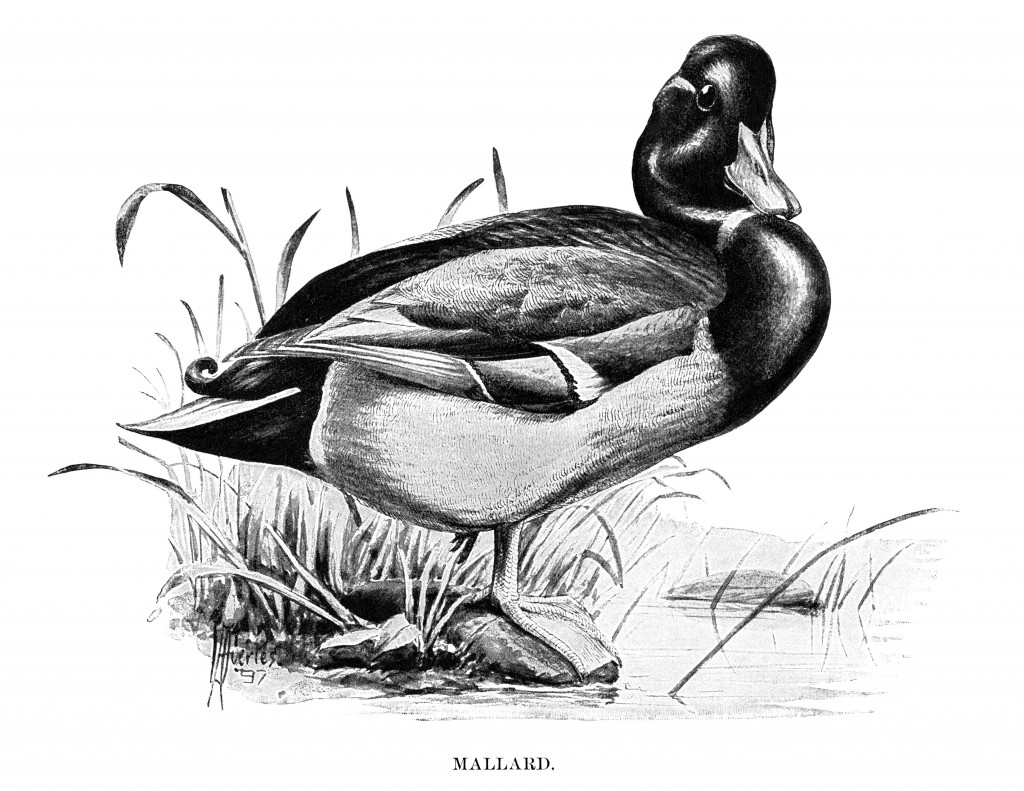
\includegraphics[width=0.45\linewidth]{figures/duck.jpg}
    \hfill
    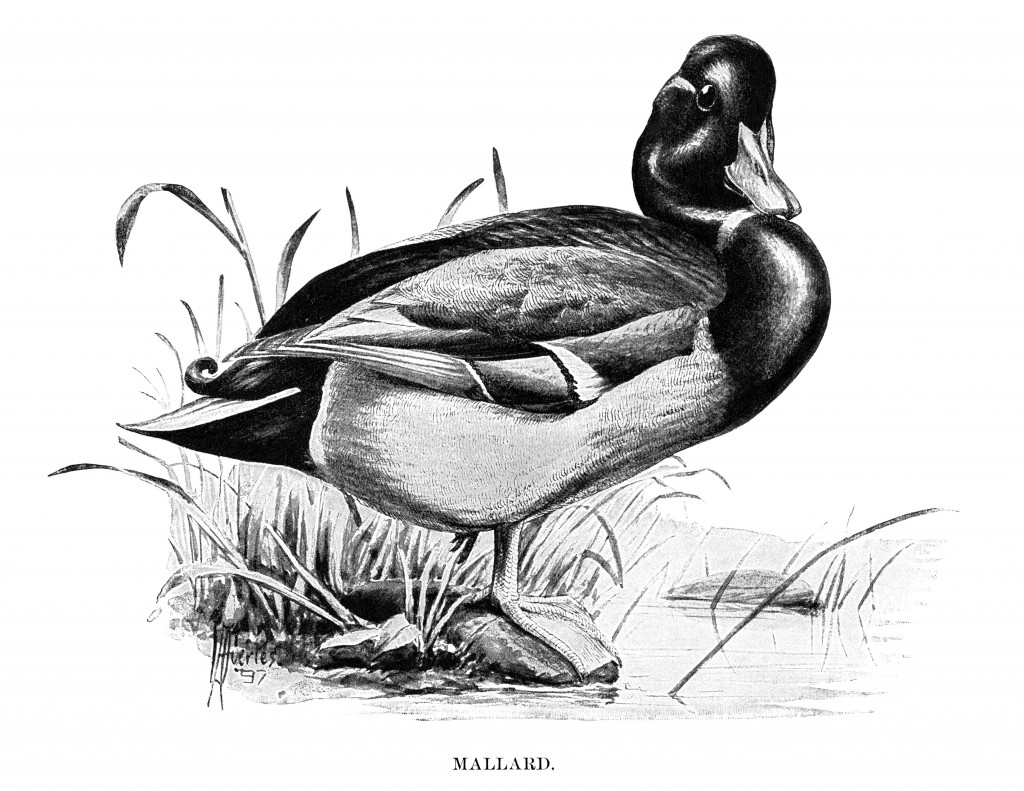
\includegraphics[width=0.45\linewidth]{figures/duck.jpg}
    \caption{(Left) Distribution of file size reduction across 1,200 Excel sheets. (Right) Runtime ratio of different approaches (lower is better).}
    \label{fig:reduction}
\end{figure}

\subsection{Implications and Discussion}
Our results highlight how streaming-based partial XML transformations can outperform naive DOM/SAX approaches in both memory use and speed. By coupling chunk-based processing with style metadata, we reliably preserve layout and avoid the “broken formatting” issue encountered in many other bloat-reduction tools.












\section{Methodology4}
\label{sec:methodology4}

 

Our methodology originated from an initial DOM-based prototype, the \emph{Excel Shrink Analyzer}, which was used to examine and understand the causes of file bloat in large Excel files. This analysis revealed that excessive file sizes were primarily caused by hidden rows, empty but styled cells, bloated shared strings, and unnecessary columns.

Due to frequent memory constraints and poor scalability when using XML-based approaches, we transitioned to a \emph{stream-based approach}. This transition was motivated by the observation that an efficient processing model could be implemented using \emph{regex-based chunk processing} on the raw bytestream. To achieve this, it was necessary to maintain a small buffer that tracked essential context such as row and column states and style references.

To construct effective regular expressions, we recognised that a simple approach was insufficient due to the hierarchical nature of Excel's XML structure. Instead, we developed a pipeline consisting of multiple regex stages, each designed to target a specific inefficiency in the spreadsheet data. The key processing steps in this pipeline are as follows. First, we identify whitespace-only shared strings and remove their referencing cells if they do not have a visible style applied. Next, we delete purely empty cells that lack any borders or fill styles. Following this, we truncate rows and columns that fall outside the bounding box of the visible data region. Lastly, we prune unnecessary column definitions while ensuring that the final column set remains extended to \texttt{XFD}, the maximum column index in Excel, in order to preserve the overall layout.

This systematic approach allows for efficient, scalable reduction of Excel file sizes without requiring large in-memory representations, thereby significantly improving both performance and storage efficiency.





Um Die Geschwindigkeit des parsens deutlich zu verbessern nutzen wir multithreading. Dabei wird für jeden der zu parsenden XML-Dateien ein eigener Thread gestartet, der die Datei verarbeitet und da jeder thread die enorm großen arbeitsblatt worksheetX.xml Dateien in kleine Chunks aufteilt und diese dann nach und nach abarbeitet, verwendet jeder dieser thread nur eine unsignifiante größe an arbeisspeicher, was im vergleich zu unserem vorherigen Setup mit dom parsern eine deutliche verbesserung darstellt, denn da war es so, dass ein einziger thread die Arbeitsblätter nacheinander abgearbeitet hat und mit einem domparser versucht hat die gleichen Dateiinhalte zu bereinigen, die unser neues programm nun auch bereinigt, doch dieser eine thread hat während dieses prozesses die meiste zeit 100 prozent des arbeitsspeichers unserer testmaschiene ausgelastet, was uns die hoffnung, den prozess automatisieren zu können zunichte machte. Unser neues Vorgehen ermöglicht es uns, die Rechenzeit signifikant zu reduzieren und die Dateien schneller zu verarbeiten. Nachfolgend ist der Algorithmus zu sehen nachdem die die Inputstreams aus der Archivdatei, welche superschnell geöffnet werden kann, da sie beim öffnen nur metainformationen über die dateien, aber nicht bereits die dateiinhalte selbst enpacken muss, jedenfalls öffnet sich dieses archiv sehr schnell und dann werden die einzelnen Inputstreams der sheetX.xml Dateien den  einzelen threads übergeben:

\begin{algorithm}[ht]
  \caption{Processing and Cleaning Excel Files in Place}
  \label{alg:process_xlsx_in_place2}
  \begin{algorithmic}

    \STATE \textbf{Input:} 
    \STATE \quad \texttt{InP} $\leftarrow$ Excel file path
    \STATE \quad \texttt{OutP} $\leftarrow$ Output path
    \vspace{0.2cm}
    
    \STATE \texttt{InArc} $\leftarrow$ Open the ZIP archive \texttt{InP} for reading
    \STATE \texttt{OutArc} $\leftarrow$ Create a new ZIP archive for writing
    \STATE \texttt{ShStr} $\leftarrow$ Extract Shared strings  from \texttt{sharedStrings.xml}
    \STATE \texttt{Sty} $\leftarrow$ Extract Styles from \texttt{styles.xml}
    \STATE \texttt{SF} $\leftarrow$ List of all sheet XML files in \texttt{Arc}
    \STATE \texttt{NSF} $\leftarrow$ List of non-sheet files in \texttt{Arc}    \vspace{0.2cm}

    \STATE \texttt{wvp} $\leftarrow$ dynamicly create pattern based on \texttt{ShStr} to identify cell values that are whitespace
    \STATE \texttt{icp} $\leftarrow$ dynamicly create pattern based on \texttt{Sty} to identify cells that are invisible
    \STATE \texttt{sdcp} $\leftarrow$ dynamicly create pattern based on \texttt{Sty} to identify cells their styles depend on the style of their column and or row style 

    \STATE \FOR{each sheet file \texttt{sf} in \texttt{SF} in parallel}
        \STATE Clean sheet file \texttt{sf} streambased using \texttt{wvp}, \texttt{icp}, \texttt{sdcp} and \texttt{Sty}
        \STATE Write cleaned sheet back to ZIP archive \texttt{OutArc}
    \ENDFOR

    \STATE \FOR{each non-sheet file \texttt{nsf} in \texttt{NSF}}
        \IF{\texttt{nsf} is \texttt{workbook.xml}}
            \STATE Clean workbook metadata with DOM
            \STATE Write cleaned workbook to ZIP archive \texttt{OutArc}
        \ELSE
            \STATE Copy file non-sheet file \texttt{nsf} unchanged to ZIP archive \texttt{OutArc}
        \ENDIF
    \ENDFOR

    \STATE \textbf{Output:} Cleaned Excel file

  \end{algorithmic}
\end{algorithm}



 

\subsection{Methodology (High-Level State-Machine Overview)}

Wie bereits erwähnt, verwendet unser neuer ansatz eine zustandsmaschiene die uns erkaubt die komplexität der operationen, die wir vornehmen um die Dateiabschnitte und die darin anzuwendenden regulären Ausdrüce im Überblick zu behalten. Die Zustandsmaschiene stellt die übersicht über die verschiedenen Schritte dar, die wir durchführen, um die Datei zu bereinigen. Die Zustandsmaschiene ist in mehrere Zustände unterteilt, die jeweils einen bestimmten Abschnitt der Datei repräsentieren, den wir gerade bearbeiten. Der Algorithmus ist nachfolgend zu sehen:  






\begin{algorithm}[ht]
  \caption{Streaming-Based Cleaning of Excel Sheet Data}
  \label{alg:clean_sheet_stream}
  \begin{algorithmic}

    \STATE \textbf{Input:} 
    \STATE \quad \texttt{SheetS} $\leftarrow$ Sheet XML stream
    %\STATE \quad \texttt{wvp} $\leftarrow$ Pattern for whitespace values
    %\STATE \quad \texttt{icp} $\leftarrow$ Pattern for invisible cells
    %\STATE \quad \texttt{sdcp} $\leftarrow$ Pattern for cells dependent on row/column styles
    %\STATE \quad \texttt{Sty} $\leftarrow$ Extracted style definitions
    \vspace{0.2cm}

    \STATE \textbf{Initialize:}
    \STATE \quad \texttt{Buffer} $\leftarrow$ Empty buffer
    \STATE \quad \texttt{Output} $\leftarrow$ Empty buffer
    \STATE \quad \texttt{State} $\leftarrow$ BEFORE\_COLS
    \STATE \quad \texttt{MaxRow} $\leftarrow$ 0
    \STATE \quad \texttt{MaxCol} $\leftarrow$ 0
    \vspace{0.2cm}

    \STATE \textbf{Processing Sheet Stream}
    \WHILE{\texttt{State} $\neq$ END\_OF\_FILE}
        \STATE Read chunk from \texttt{SheetS} into \texttt{Buffer}

        \STATE \IF{\texttt{State} is in BEFORE\_COLS, BEFORE\_SHEET\_DATA \\or AFTER\_SHEET\_DATA} 
            \IF{Found \texttt{<cols>}, \texttt{<sheetData>}}
                \STATE Store \texttt{Buffer} in \texttt{Output} until last found tag
                \STATE Discard content in \texttt{Buffer} until last found tag
            \ENDIF
            \IF{Found \texttt{<cols>}}
              \STATE \texttt{State} $\leftarrow$ IN\_COLS
            \ELSIF{Found \texttt{<sheetData>}}
                \STATE \texttt{State} $\leftarrow$ IN\_SHEET\_DATA
            \ELSIF{Found end of file}
                \STATE Store whole \texttt{Buffer} in \texttt{Output} 
                \STATE \texttt{State} $\leftarrow$ END\_OF\_FILE
            \ENDIF
        \ELSIF{\texttt{State} is IN\_COLS}
            \IF{Found \texttt{</cols>} or \texttt{<col/>}}
                \STATE Parse column definitions
                \STATE Store \texttt{Buffer} in \texttt{Output} until last found tag
                \STATE Discard content in \texttt{Buffer} until last found tag
            \ENDIF
            \IF{Found \texttt{</cols>} }
                \STATE \texttt{State} $\leftarrow$ BEFORE\_SHEET\_DATA
            \ENDIF
        \ELSIF{\texttt{State} is IN\_SHEET\_DATA}
            \IF{Found \texttt{"</row>"}, \texttt{"<row .../>"} or \texttt{</sheetData>}}
                \STATE Clean \texttt{Buffer} from invisible cells/rows using patterns
                \STATE Store cleaned \texttt{Buffer} in \texttt{Output}
                \STATE Discard content in \texttt{Buffer} until last found tag
                \STATE Extract remaining cell references to update \texttt{MaxRow} and \texttt{MaxCol}
            \ENDIF
            \IF{Found \texttt{</sheetData>} }
                \STATE \texttt{State} $\leftarrow$ AFTER\_SHEET\_DATA
            \ENDIF
        \ENDIF
    \ENDWHILE
    \vspace{0.2cm}

    \STATE \textbf{Post-Processing}
    \STATE Extract and update \texttt{MaxRow} and \texttt{MaxCol} from merge cells
    \STATE Remove rows exceeding \texttt{MaxRow} from \texttt{SheetData}
    \STATE Merge extraneous columns beyond \texttt{MaxCol}
    \vspace{0.2cm}

    \STATE \textbf{Output:} Cleaned sheet XML

  \end{algorithmic}
\end{algorithm}





We implement our spreadsheet parser as a streaming-based state machine, where each chunk of XML data is processed incrementally to minimise memory consumption and to permit early discarding of unwanted parts of the file. Both our “consecutive” and “interleaved” parsing approaches, which saves memory usage, use this same underlying state machine. In the description below, we focus specifically on how our parser transitions between states (i.e., how each state-changing function decides to advance to a new state), deferring the lower-level details of what happens \emph{within} each state until later sections.

\paragraph{States}
We define six primary states in our parser:
\begin{itemize}
  \item \texttt{BEFORE\_COLS}: The parser has not yet encountered the \mbox{\texttt{\textless cols\textgreater}} element. It searches for either \mbox{\texttt{\textless cols\textgreater}} or \mbox{\texttt{\textless sheetData\textgreater}} in the stream.
  \item \texttt{IN\_COLS}: The parser has found \mbox{\texttt{\textless cols\textgreater}} and is now processing column definitions.
  \item \texttt{BEFORE\_SHEET\_DATA}: The parser has finished reading (or did not find) the \mbox{\texttt{\textless cols\textgreater}} node and looks for the first \mbox{\texttt{\textless sheetData\textgreater}} element.
  \item \texttt{IN\_SHEET\_DATA}: The parser is processing the main worksheet data, including row and cell elements.
  \item \texttt{AFTER\_SHEET\_DATA}: The parser has found the closing \mbox{\texttt{\textless /sheetData\textgreater}} and is gathering any subsequent chunks, typically until the end of the file.
  \item \texttt{END\_OF\_FILE}: The parser has reached the end of the stream. No further parsing is required.
\end{itemize}


\paragraph{1.\ \texttt{collect\_chunks\_until\_cols\_sheet\_data\_or\_end\_of\_stream}} 
While the parser is in \texttt{BEFORE\_COLS}, \texttt{BEFORE\_SHEET\_DATA}, or \texttt{AFTER\_SHEET\_DATA}, this function tries to find specific tag boundaries (e.g., \verb|<cols>|, \verb|<sheetData>|, or \verb|</cols>|). When it detects such a tag at position \verb|i| in the buffer:
\begin{enumerate}
  \item It \emph{cuts} the buffer at \verb|i|, meaning it splits the buffer into two segments: 
   \emph{(1)} the portion from the start of the buffer through the end of that tag (the ``clean cut''), and 
   \emph{(2)} whatever bytes remain \emph{after} that tag.
  \item It returns the first segment as \texttt{chunk\_to\_add} (which the parser immediately outputs or processes for the current state).
  \item The second segment becomes the \emph{updated buffer}, ensuring that the relevant XML node boundary is never cut in half. 
\end{enumerate}
If the function \emph{fails} to find the tag it is looking for, it returns \texttt{None} for both the new chunk and the new state; \emph{no} modification is done to the buffer. This design permits the next incoming chunk of data to be appended to the unchanged buffer in the following iteration, eventually providing enough content to match the desired tag boundary.

\paragraph{2.\ \texttt{collect\_cols\_chunks\_and\_parse\_cols}}
When the parser is in \texttt{IN\_COLS}, this function specifically searches for \verb|</cols>| or, failing that, for one or more \verb|<col .../>| elements. On detecting \verb|</cols>|, it cuts the buffer right \emph{before} that closing tag and transitions to \texttt{BEFORE\_SHEET\_DATA}. If the function does not find the closing tag but does discover complete \verb|<col .../>| elements, it consumes them (again as a clean cut) and leaves the parser in \texttt{IN\_COLS} to continue. As before, if no relevant match is found at all, the buffer is unaltered so that subsequent chunks can be appended for a future match attempt.

\paragraph{3.\ \texttt{collect\_only\_visible\_row\_and\_cell\_chunks\_and\_calculate\_sheet\_dimensions}}
When parsing the main sheet data in \texttt{IN\_SHEET\_DATA}, we similarly look for \verb|</sheetData>| or row boundaries. We locate the boundary of a row (either a self-closing form, \verb|<row .../>|, or an open--close form, \verb|<row ...>...</row>|). If \verb|</sheetData>| is found, the function cuts the buffer at that tag and transitions the parser to \texttt{AFTER\_SHEET\_DATA}. If no row boundary or closing tag is yet fully contained in the buffer, it remains unmodified so that the next chunk from the file can complete the row or \verb|sheetData| boundary.


\subsubsection{Ensuring ``Clean Cuts'' within the Streaming Buffer}
Our parser reads the raw XML data incrementally into a working \emph{buffer} and ensures that each XML node boundary is cleanly preserved, so that no node is split across two chunks. Each state-transition function handles this in a slightly different way, as described below. However, the shared principle is that the parser only performs a ``cut'' in the buffer if it has already read enough bytes to match one of the relevant XML tags (e.g., \verb|<cols>| or \verb|</sheetData>|). If none of the looked-for tags appear yet, \emph{no} cut is made: the function returns without changing the buffer, so the parser simply appends the next chunk to the existing buffer and tries again.


\paragraph{Buffer Updates and State Progress}
By constraining all parsing decisions to these well-defined cuts, the parser never splits an XML node across separate buffers. Each function either (1)~makes a precise cut on the matching tag boundary (and updates the parser state accordingly), or (2)~leaves the buffer untouched if no boundary is found, ensuring the remainder of the stream can be appended in the subsequent iteration. This incremental procedure allows the parser to operate in a memory-efficient streaming manner while guaranteeing well-formed XML segments in each extracted chunk.
 

\paragraph{Putting It All Together.}
By orchestrating these transitions, the parser incrementally identifies the \mbox{\texttt{\textless cols\textgreater}} segment (if present) and the main \mbox{\texttt{\textless sheetData\textgreater}} block. Once \mbox{\texttt{\textless /sheetData\textgreater}} is found, it switches to a final phase to read any trailing data without further parsing. When no more data remains, it enters \texttt{END\_OF\_FILE}. Later sections detail how, \emph{within} each state, we selectively discard or retain rows, cells, and styles, ultimately producing a more compact file representation.

 Das Heavy Lifting spielt sich in der Bereinigung der Daten im SheetData node ab. In unserer Analyse befanden sich hier die meisten ursachen für file bloat. Die Bereinigung geht foldendermaßen von statten:
 

 

\noindent \textbf{Overview.} This sequence of transformations streamlines an XML-based spreadsheet by removing superfluous cell entries and entire rows that do not contribute to the visible content or formatting of the sheet. In particular, it eliminates cells whose sole content is whitespace, cells that reference a style providing only a basic font (i.,e.\ no genuine fill or border), and rows that have no meaningful content.



\subsection{Optimization of Shared String References}

In the Open XML format used by Excel workbooks, textual data is managed through a shared string table stored in \texttt{sharedStrings.xml}. This structure ensures that identical strings appearing multiple times across the workbook are stored only once, reducing redundancy. However, whitespace-only entries may still be retained in the shared string table, leading to unnecessary storage overhead.

\subsubsection{Identification of Empty String Entries}
The optimization process begins by scanning the shared string table to identify entries consisting solely of whitespace characters. The indices corresponding to these redundant entries are recorded for later removal. Since Excel does not automatically eliminate such empty references, their presence can contribute to inefficient memory usage.

\subsubsection{Pattern-Based Detection and Removal}
To efficiently eliminate these references from the worksheet data, the identified indices are transformed into a structured regular expression. This regular expression is constructed as an alternation pattern, where multiple indices are combined into a single pattern separated by the logical OR operator (\texttt{|}). The resulting pattern is designed to match instances of \texttt{<v>} elements within the worksheet XML that reference these indices.

\subsubsection{Application to Sheet Data}
Once the regular expression pattern is prepared, it is applied to the worksheet XML to locate and remove all occurrences of \texttt{<v>} elements referencing whitespace-only strings. This step effectively clears the affected cell entries, reducing the overall file size without modifying meaningful data.

\subsubsection{Efficiency Considerations}
This approach is particularly efficient as it operates directly on the raw XML representation of the workbook, leveraging regular expressions for bulk modifications in a single pass. By precompiling the regular expression and applying it to the XML stream, the transformation process remains computationally efficient even for large datasets. 

The elimination of redundant entries leads to a significant reduction in storage requirements while preserving the semantic correctness of the spreadsheet. This optimization is especially beneficial in large-scale datasets, where excessive whitespace can substantially contribute to file bloat.




\subsection{Elimination of Redundant Cell Style References}

In Excel's Open XML structure, cells reference styles defined in the \texttt{cellXfs} section of the \texttt{styles.xml} file. Often, cells may reference styles that specify only font properties without any distinct fill or border attributes. Such references can be superfluous, especially when the default formatting suffices. The following optimization targets the removal of these redundant style references to streamline the workbook's XML structure.

\subsubsection{Identification of Minimal Style Definitions}
The process initiates by analyzing the \texttt{cellXfs} list to pinpoint style definitions that lack custom fill and border settings. Specifically, it compiles a list of style indices where both \texttt{fill\_id} and \texttt{border\_id} are either unset or set to their default values (typically zero), and the corresponding \texttt{apply\_fill} and \texttt{apply\_border} flags are \texttt{False}. These indices represent styles that modify only font attributes without altering cell fill or borders.

\subsubsection{Regular Expression Construction for Cell Matching}
With the indices of these minimal styles identified, a regular expression pattern is constructed to detect cells in the worksheet XML that reference them. The pattern searches for cell elements (\texttt{<c>}) possessing a style attribute (\texttt{s}) matching any of the identified indices. The regular expression is carefully crafted to ensure precise matching, accounting for word boundaries and attribute delimiters to avoid partial or erroneous matches.

\subsubsection{Substitution to Remove Redundant References}
Applying the constructed regular expression to the worksheet's XML content, all matching cell elements are identified. These elements are then removed or their style attributes cleared, effectively eliminating unnecessary style references. This cleanup reduces the complexity of the XML structure and can contribute to a reduction in the overall file size.

\subsubsection{Efficiency and Impact}
This method leverages Python's regular expression capabilities to perform targeted substitutions within the XML content. By focusing on specific patterns corresponding to redundant style references, the approach ensures that only superfluous data is removed, preserving the integrity and appearance of the worksheet. The optimization is particularly beneficial in workbooks with numerous cells referencing default or minimal styles, as it streamlines the XML and enhances processing efficiency.







\subsection{Deleting Invisible Cells}

Because we already deleted whitespaces, and then we found every cell, that has no value anymre, either, because we deleted the whitespace frm that cell, or because that cell never had any conent and got nonetheless a style applied that is only related to text.
Because we already did all that, all that we can delete now are cells that have no visible style applied to them, that is, cells that have no border and no fill.
However, this is not as easy as it sounds, because the style of a cell is not only determined by the style of the cell itself, but sometimes also by the style of the row and the style of the column that the cell is in.
The cell style indicates this detail with its applyFill and applyBorder flags. If these flags are set to true, then that means that either the correspondig column or the corresponding row, or even both have a border or fill or both and applyFill orders the cell to overwrite the style of the column or row with something different.
This is what this feature really is for. Because Excel allows to apply a border or a fill to a whole row or a whole column,. This actually saves filesize, because otherwise each of the cells 
the cell has a fill and a border, respectively, that is different from the fill and border of the row and the column that the cell is in that row or column would need to have the corresponding style applied which is too much if there are (put in here the max amount of possible columns and possible rows in a excel sheet.)
With that feature the user can just tell excel, that the column has a certain style. and only one style definition is saved for that style.
However, stellen sie sich folgendes vor. Sier färben eine ganze Spalte in einer farbe, dann färben sie eine ganze Zeile in einer anderen farbe. Sie werden natürlich daran denken müssen, dass sich diese spalte und zeilen in einer zelle treffen. Woher weiß die Zelle welchen style sie anwenden soll?
Den von der spalte oder den von der Zeile. Um diese Frage zu beantworten arbeitet excel für diese styles die der celle zugewiesen sind mit dem Attribut applyFill und applyBorder. If those attributes are set, then the cell knows it should apply its fill or border. Normalerweise sollte in diesen Fällen dann die fillId oder die borderId eine andere sein, als die des rows oder columns. Doch wir haben in unserer Analyse sehr häufig festgestellt, dass viele solcher Zellen die ANweisung haben, den Style der Row oder Column anzuwenden, doch die borderId und oder die fillId waren identisch. Das kann dem nutzer durch fehlerhafte bedienung passiert sein. Zunächst hat der Nutzer vielleicht nur die Zellen angewählt, um sie zu färben oder ihnen eine border zu geben und später entschied sich der Nutzer, die ganz Spalte oder die ganze Zeile zu färben oder zu umranden. Doch die Zellen haben den Style der Spalte oder der Zeile nicht überschrieben. Das ist ein Fehler, der in Excel passieren kann. Doch wir haben festgestellt, dass dieser Fehler sehr häufig passiert. Deshalb haben wir uns entschieden, diese Zellen zu löschen, wenn sich durch die Löschung keine Visuelle Änderung ergibt. 
In out algorith we determine whether a given cell’s overall visual styling (in terms of fills and borders) is effectively “invisible,” and if so, removes the corresponding cell entry from the worksheet.
 We do so by jointly examining three distinct style properties for the cell: (i) the explicitly assigned cell style, (ii) the row-level style, and (iii) the column-level style. Each of these styles can indicate whether the cell is supposed to apply a fill (via an applyFill flag) and/or a border (via an applyBorder flag), and each style points to a fill object (identified by fillId) and a border object (identified by borderId). The procedure proceeds as follows:

Identify Cell, Row, and Column Styles.
First, the algorithm determines which cell, row, and column are being examined. The cell itself includes a reference to the style index (indicated by the s attribute which points to the corresponding xf in the styles.xml) identifying its own borderId and fillId. In parallel, the row and column that contain this cell may also define their own style indices, including row-specific or column-specific borderId/fillId .

Check Whether a Border Is Actually Present.

If row and column both say applyBorder is set, the algorithm compares the cell’s borderId against the row’s borderId and the column’s borderId. A discrepancy (i.e., the cell’s borderId differs from the row’s or column’s) implies a genuinely visible border. If the IDs match exactly, it suggests the border effect might already be uniformly defined at the row or column level, so the algorithm regards the cell’s own border as non-unique.
If only a row or only a column indicates applyBorder, then the cell’s borderId is contrasted with whichever one applies. If they differ, that also signifies a special border visible at the cell.
If the border object has no visible lines, the algorithm concludes also that there is no border.

Check Whether a Fill Is Actually Present.

If a cell has  applyFill set, then the fillId from the cell is checked against the row’s and column’s fillId. A difference signifies an explicit cell fill that supersedes the row or column fill; identical IDs mean the fill effect was inherited from row or column, not newly introduced by the cell.
If only a row or only a column indicates applyFill, the algorithm checks whether the cell’s fillId differs from that row or column fillId. If it does, it implies a distinct fill is being applied.
If there is no indication of applyFill at the row or column, the procedure inspects the cell’s fill object: specifically, it looks for the pattern fill (for example, a patternFill element) and checks whether the patternType is something other than “none.” A “none” pattern means that no visible fill is present.

Remove the Cell If No Visible Style Exists.
Finally, if these checks show that the cell does not have its own distinguishable border or fill, and it also does not inherit any visible border or fill from its row or column, then the cell’s reference is removed entirely from the underlying XML data. Otherwise, the cell remains.

By combining row-level, column-level, and cell-level style signals—particularly via applyFill, applyBorder, fillId, and borderId—this procedure ensures that cells carrying no genuinely visible formatting (no practical fill or border) are omitted. This helps eliminate extraneous markup in the spreadsheet file without changing the visual appearance of the resulting worksheet.
 
Overall, this procedure reduces the file size significantly by eliminating redundant or wholly invisible XML elements, with no loss to the spreadsheet’s displayed content. By leveraging the \texttt{applyFill}, \texttt{applyBorder}, and related identifiers (\texttt{fillId}, \texttt{borderId}), it precisely distinguishes cells and rows that are visually relevant from those that are not.


\subsection{Removal of Empty Rows in Worksheet XML}

In the process of optimizing Excel workbooks stored in the Open XML format, it is essential to eliminate superfluous elements that do not contribute to the workbook's content. One such optimization involves the removal of empty \texttt{<row>} elements from the worksheet's XML data. These empty rows can unnecessarily bloat the file size and complicate data processing.

\subsubsection{Regular Expression Pattern for Identifying Empty Rows}

To detect and remove empty \texttt{<row>} elements, a regular expression pattern is constructed. This pattern specifically targets \texttt{<row>} tags that do not contain any cell (\texttt{<c>}) elements or data. The regular expression is defined as follows:

%\begin{verbatim}
%\texttt{PATTERN\_EMPTY\_ROWS = re.compile(}
%\texttt{    rb'<row(?=(?:\s+(?:r|spans)="[^"]*")*\s*>)(?:\s+(?:r|spans)="[^"]*")*\s*>\s*</row>'}
%\texttt{)}
%\end{verbatim}

This pattern operates by:

\begin{itemize}
    \item Matching a \texttt{<row>} tag that may include attributes such as \texttt{r} (row number) or \texttt{spans}.
    \item Ensuring that the \texttt{<row>} tag is immediately closed without containing any nested elements or text, indicating an empty row.
\end{itemize}

\subsubsection{Applying the Pattern to Remove Empty Rows}

Once the pattern is defined, it is applied to the worksheet's XML content to identify and remove all instances of empty rows. This is achieved through the substitution method:

\begin{verbatim}
\texttt{processed\_chunk = PATTERN\_EMPTY\_ROWS.sub(b"", processed\_chunk)}
\end{verbatim}

In this context, \texttt{processed\_chunk} represents a segment of the worksheet's XML data being processed. The \texttt{sub} method replaces all matches of the pattern (i.e., empty \texttt{<row>} elements) with an empty byte string, effectively removing them from the XML content.

\subsubsection{Benefits of Removing Empty Rows}

Eliminating empty rows from the worksheet's XML offers several advantages:

\begin{itemize}
    \item \textbf{Reduced File Size:} By removing unnecessary elements, the overall size of the Excel file is decreased, leading to more efficient storage and transmission.
    \item \textbf{Improved Performance:} Streamlining the XML structure can enhance the performance of applications that process or render the workbook, as there are fewer elements to handle.
    \item \textbf{Enhanced Readability:} A cleaner XML structure facilitates easier maintenance and debugging, as the content is more concise and devoid of redundant elements.
\end{itemize}

This optimization is particularly beneficial in scenarios where workbooks are generated or manipulated programmatically, and extraneous empty rows may be inadvertently introduced. By incorporating this regular expression-based approach, such superfluous elements can be systematically identified and removed, ensuring the workbook remains efficient and well-structured.


Nachdem wir die meisten der unsichtbaren Zellen gelöscht haben, bleiben einerseits noch die Zeilen übrig, die in gewisser weise einen style haben, da ihnen eine höhe zugewiesen ist. Würde man diese Zellen einfach so löschen, nur weil sie einen style zugewiesen haben, würde sich das layout des sheets verändern. Ähnliches kilt für Spaltendefinitionen in der Cols-Node Section. Dieses haben wir zuvor nur geparsed aber darin nichts bereinigt.
Diese Bereinigungen sind nur jetze möglich, nun da wir alle cellen gelöscht haben, die keinen sichtbaren style und keinen Wert haben. Damit sind alle Zellen gelöscht, die keinen sichtbaren Inhalt haben. Alle Zeilen die Unterhalb dieser übrig bleibenden wichtigen Zellen liegen, können keinen Inhalt verschieben, weil sie beisppielsweise eine zugewiesene Höhe haben und  können deshalb gelöscht werden. Das gleiche gilt für die Spalten in der Cols-Node Section. Alle SPalten, die sich Rechts von den übrig gebliebenen wichtigen Zellen befinden, können keinen Inhalt verschieben und können deshalb gelöscht werden. Deshalb haben wir zuvor im SHeetData Node die MaximaleZeile und die Maximale Spalte getrackt, um nun alles zu löschen was sich rechts und unterhalb davon befindet.
 
\section{Implementation}
\label{sec:implementation}

We implemented our streaming approach as a Python tool named \emph{Excel Shrink} (publicly available via GitHub\footnote{\url{https://github.com/...}}). Below, we highlight key aspects:

\paragraph{Archive-Wide Streaming.} We open the \texttt{.xlsx} (ZIP container) and process each subfile. Non-XML subfiles (images, macros) are passed through unmodified. For each XML subfile, we:

\begin{enumerate}
    \item Read in small chunks (e.g.\ 8--64\,KB) and maintain a \emph{rolling buffer} that ends exactly at XML tag boundaries relevant for transformations. 
    \item Use a \emph{state machine} (e.g.\ \textsc{BeforeColsNode}, \textsc{InColsNode}, \textsc{InSheetDataNode}, etc.) to trigger different sets of regex replacements on each chunk.
    \item Patch the chunk in place, removing or editing text nodes, then write out the result to a new ZIP stream. 
\end{enumerate}

\paragraph{Multiprocessing.} 
To exploit modern multi-core CPUs, we parallelise the processing of large worksheets. Each sheet is streamed in a separate Python process, minimising memory overhead. We rejoin them in the final ZIP seamlessly.

\paragraph{Metadata Handling.}
We partially parse only \texttt{styles.xml} and \texttt{sharedStrings.xml}, building minimal dictionaries of border/fill references and textual content indices. This small overhead is required to decide if an empty cell is truly invisible or if it has a visually significant style.

\paragraph{Performance vs.\ Full Parsing.}
SAX-based or DOM-based code can require hundreds of seconds (or fail entirely) on multi-gigabyte expansions of a “.xlsx.” In contrast, we keep each chunk under 100\,KB, apply local transformations, and forward the rest unparsed. 

\section{Evaluation}
\label{sec:evaluation}

We tested our approach on 1,200+ real Excel files from the German Federal Statistical Office, covering year-based directories and containing numerous oversize spreadsheets. We also compared performance to:
\begin{itemize}
    \item \textbf{DOM-based approach} using \texttt{lxml} in Python
    \item \textbf{SAX-based approach} using \texttt{xml.sax}
    \item \textbf{Microsoft Excel 365 Check Performance} (manually invoked)
\end{itemize}

\paragraph{File Size Reduction.}
Figure~\ref{fig:reduction} (left) shows that 35\% of sheets were reduced by over 90\%, and 15\% of them exceeded 99\% reduction. The largest single sheet dropped from 85\,MB to 2.76\,MB, all while preserving layout and content.

\paragraph{Runtime Comparison.}
Figure~\ref{fig:reduction} (right) compares the wall-clock runtime. We normalise \emph{Excel Shrink}’s runtime to the time Excel needed just to open each file. On average, we completed the shrink \emph{20\% faster} than Excel’s open time, and in many cases, the total time for “shrink + then open in Excel” was still \emph{shorter} than opening the original file directly in Excel.

\begin{figure}[t]
    \centering
    % Replace with your own reduction and runtime plots
    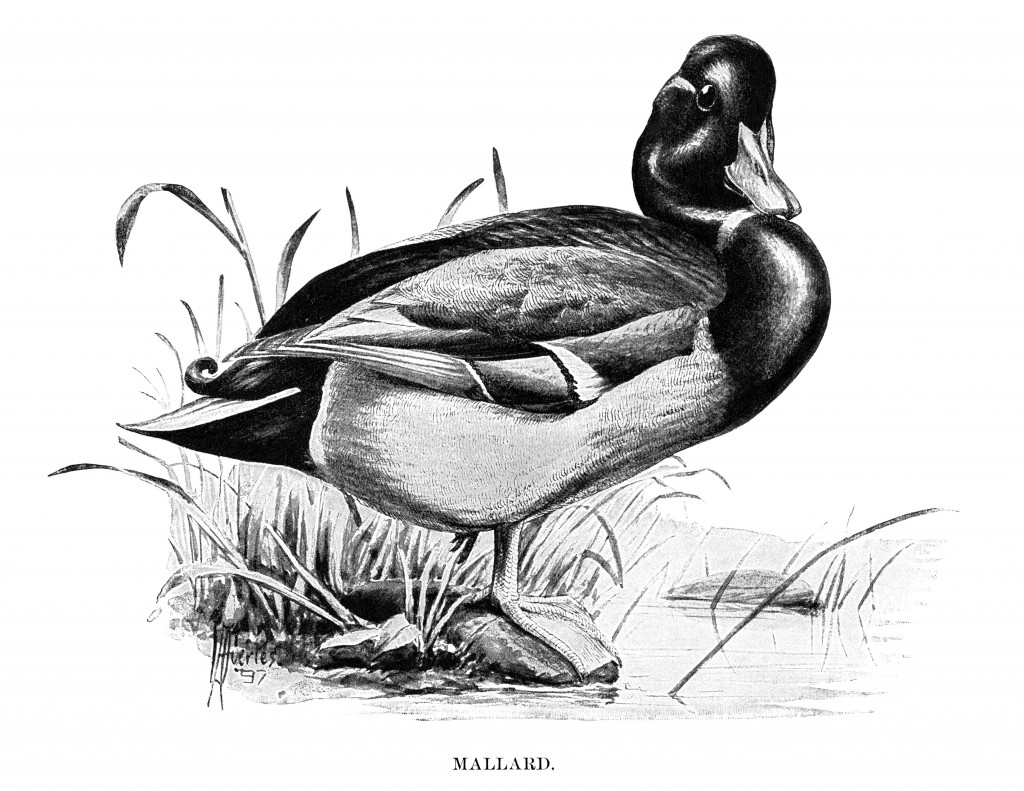
\includegraphics[width=0.45\linewidth]{figures/duck.jpg}
    \hfill
    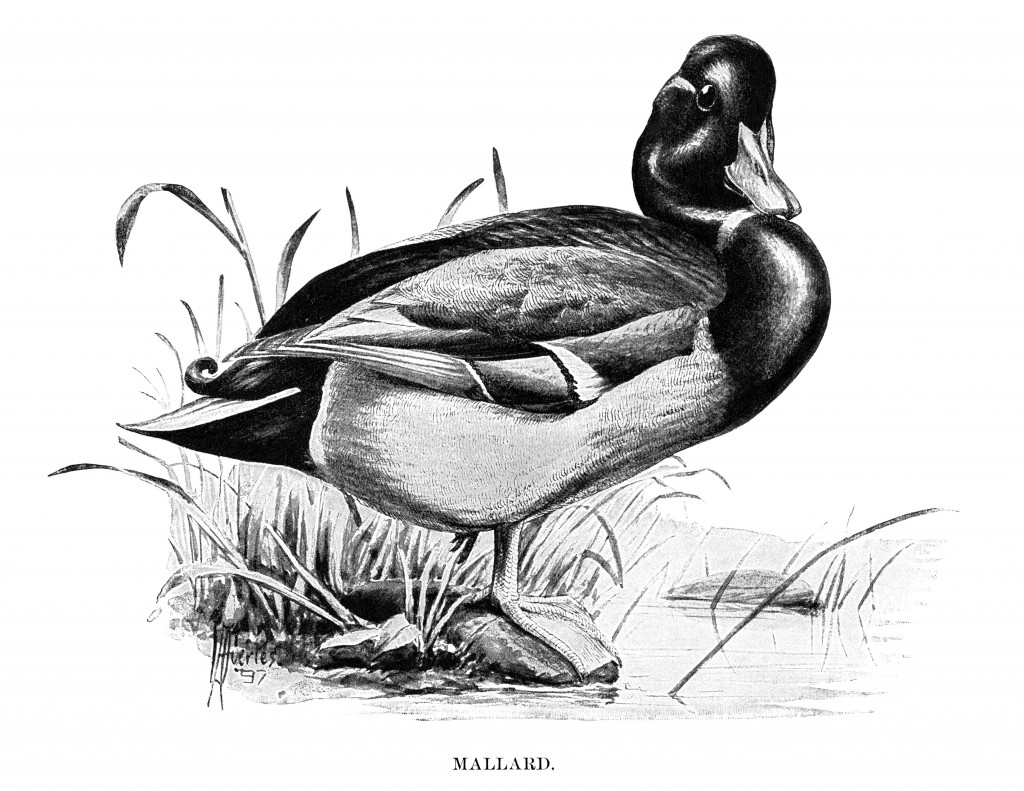
\includegraphics[width=0.45\linewidth]{figures/duck.jpg}
    \caption{(Left) Distribution of file size reduction across 1,200 Excel sheets. (Right) Runtime ratio of different approaches. Lower is better.}
    \label{fig:reduction}
\end{figure}

\subsection{Implications and Discussion}
Our results underscore that streaming partial XML transformations can surpass naive approaches (DOM/SAX) in both memory and runtime. Moreover, the synergy of chunk-based processing and style metadata ensures that we can preserve layout reliably, avoiding the “broken formatting” problem in many existing bloat-reduction tools.



\section{Conclusion}
\label{sec:conclusion}
We introduced a streaming-based, multiprocessing strategy for removing Excel file bloat at scale, demonstrating that it can outperform native Excel loading times. By combining partial XML parsing for style metadata with a pipeline of dynamic regex transformations, we preserve worksheet layout while eliminating up to 99.99\% of the storage overhead. 

Beyond Excel, our contribution highlights how domain-specific streaming transformations can circumvent memory-intensive parsing in other compressed XML-based systems. Future work includes porting our approach to lower-level languages (C++, Rust) for even higher throughput, and extending the technique to related file formats such as ODS (OpenDocument Spreadsheet). We believe that bridging the gap between domain-specific knowledge (styles, merges, hidden columns) and high-performance streaming offers a promising avenue for \emph{truly large} spreadsheet management in the broader data management community.



\bibliographystyle{ACM-Reference-Format}
\bibliography{acmart.bib}



\appendix



\section{Excel Shrink}

The objective of \textit{Excel Shrink} is to reduce the size of \textit{Excel} files by removing content that is invisible to the user and likely unintentionally included in the file. This includes empty cells, cells containing only whitespace, cells with non-visible formatting, and unused rows and columns.

\subsection{Deletion of White Spaces}

Excel users lack a straightforward method to identify which cells in a worksheet contain only whitespace characters. To highlight these whitespaces, we have marked cells containing exclusively whitespaces in red within this worksheet, which includes 4,121 such instances (see Figure~\ref{fig:whitespaces})~\cite{destatis2023Konsumausgaben5811109}.

\begin{figure}[ht]
  \centering
  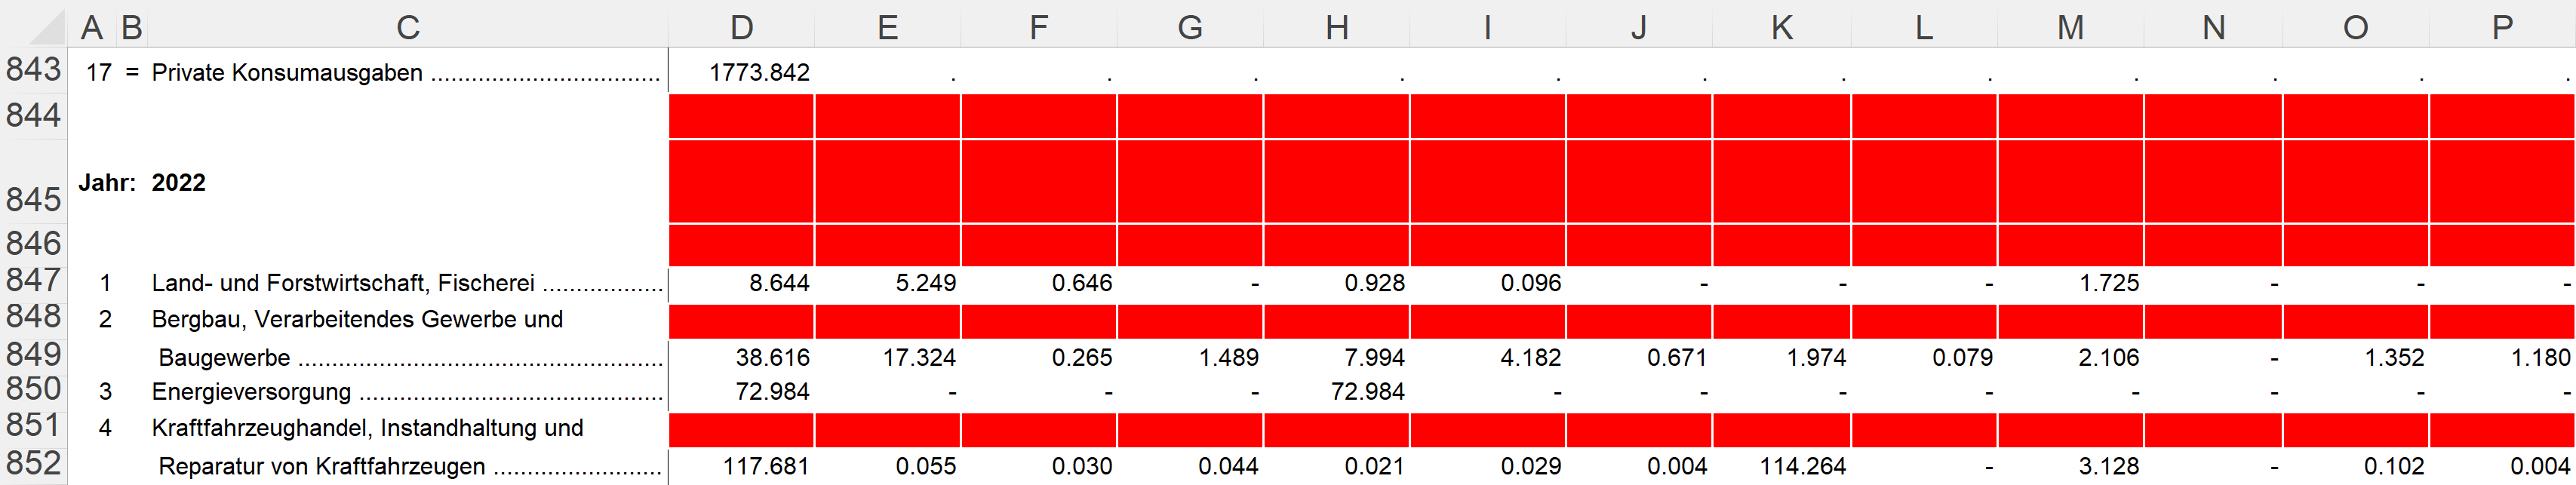
\includegraphics[width=\linewidth]{images/excel_shrink/whitespaces/whitespaces3.png}
  \caption{Cells containing only whitespaces are highlighted in red.}
  \label{fig:whitespaces}
\end{figure}%

\begin{lstlisting}[caption={Cell \texttt{D844} in \texttt{sheet28.xml}}, label={lst:whitespaces_d844}, firstnumber=48]
<row r="844" spans="1:16" ht="14.1" customHeight="1">
  <c r="D844" s="428" t="s">
      <v>102</v>
  </c>
\end{lstlisting}
To detect these whitespaces, it is insufficient to examine the cell itself, as even a single space is stored by \textit{Excel} in the file for recurring texts, even if the text appears only once in the entire \textit{Excel} file. Cell \texttt{D844} appears in the XML as shown in Listing~\ref{lst:whitespaces_d844}.

The row is marked by the \texttt{<row>} tag with the attribute \texttt{r="844"}, indicating that it is the 844th row. Within the row, the \texttt{<c>} tag represents a cell, identified by the attribute \texttt{r="D844"}. The attribute \texttt{t="s"} specifies the cell type; in this case, \texttt{s} stands for \textit{String}~\cite{openxml}.

The cell's value is stored within the \texttt{<v>} tag, where the value \texttt{102} is specified. This value is interpreted as an index in a string table, referencing a specific text in a separate list defined in the \textit{Excel} file, namely the \texttt{sharedStrings.xml} file.

Since \textit{Excel} stores even single spaces in the Shared String Table, merely inspecting the cell's content is insufficient to detect whitespaces. By examining the shared strings, we can identify entries that contain only whitespace characters or are empty, allowing us to determine which cells can be safely deleted.
To locate the value, we must search for the \texttt{<sst>} node in the \texttt{sharedStrings.xml} file, as shown in Listing~\ref{lst:sharedStringsSst}.

\begin{lstlisting}[caption={Shared String Table (\texttt{sst}) in \texttt{sharedStrings.xml}}, label={lst:sharedStringsSst}, firstnumber=48]
<sst count="17962" uniqueCount="732">
  <si>
    <t>062</t>
  </si>
  \end{lstlisting}

The provided XML excerpt displays a portion of the Shared String Table (SST) in an \textit{Excel} file~\cite{microsoft2024sharedstring}. The Shared String Table is a structure that allows for the storage and management of shared strings within an \textit{Excel} workbook. Instead of storing each string separately in every cell, each unique string is stored once in the Shared String Table. This approach saves storage space, as cells then reference these strings via indices. Each entry in this table has an ascending index number, starting at \texttt{0} for the first string, \texttt{1} for the second, and so forth. The \texttt{count} attribute indicates the total number of strings in the table, while \texttt{uniqueCount} represents the number of unique strings. In this case, there are \texttt{17,962} strings in total, of which \texttt{732} are unique. This means that many strings in the table are used multiple times.

Within the SST, there are elements of type \texttt{<si>} (Shared Item), each containing a string. In this example, the \texttt{<t>} element displays the actual text of the string stored in the table. Here, the string \texttt{062} is represented, which can be referenced by an index in a cell.

To find the string corresponding to index \texttt{102}, we must look for the 103rd entry (since indexing starts at 0), which is shown in Listing~\ref{lst:whitespacesSi}.

\begin{lstlisting}[caption={Empty string at index 102 in \texttt{sst}}, label={lst:whitespacesSi}, firstnumber=48]
<si>
  <t xml:space="preserve"></t>
</si>
\end{lstlisting}

Within the \texttt{<si>} element is a \texttt{<t>} element containing the actual text of the string. In this specific case, the content of the \texttt{<t>} element is empty, indicating that no text is stored. The attribute \texttt{xml:space="preserve"} suggests that this represents a whitespace character. Therefore, all cells referencing index \texttt{102} for the reusable string can be deleted, as they contain no visible content.


\subsection{Deletion of Empty Columns}

The first indication of excessive column definitions can be observed in the horizontal scrollbar when opening the worksheet, as shown in Figure~\ref{fig:col_scrollbar_arrow}~\cite[Sheet: \texttt{0902\_T\_NW}]{destatis2023Foerderprogramme}. If the entire data range is already within the visible area and yet the scrollbar thumb is very narrow and small compared to the scrollable area, it indicates that a large number of column definitions are making the worksheet significantly wider than the actual data range.
Scrolling into this area, the user may notice that among columns with uniform widths, some columns occasionally have differing widths, as shown in Figure~\ref{fig:col_s_arrow}.


  
\begin{figure}[ht]
  \centering
  \begin{subfigure}[b]{0.48\linewidth}
    \centering
    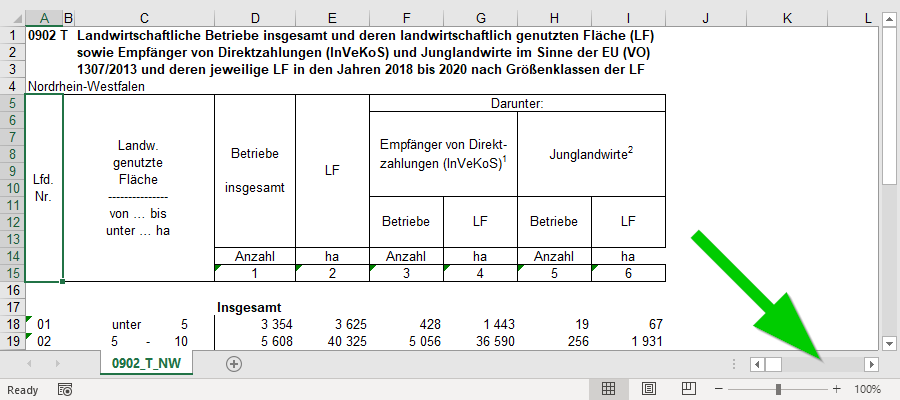
\includegraphics[width=\textwidth]{images/excel_shrink/cols/col_scrollbar_arrow.png}
    \caption{Very wide scrollable area and very narrow scrollbar thumb}
    \label{fig:col_scrollbar_arrow}
  \end{subfigure}
  \hspace{0.01\linewidth} % Space between images
  \begin{subfigure}[b]{0.48\linewidth}
    \centering
    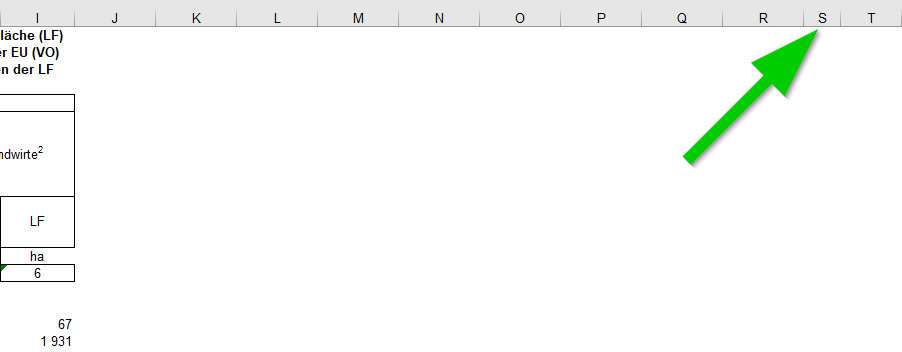
\includegraphics[width=\textwidth]{images/excel_shrink/cols/col_s_arrow.png}
    \caption{Custom Column Width for a Column Outside the Data Range}
    \label{fig:col_s_arrow}
  \end{subfigure}
  \caption{}
  \label{fig:col_scrollbar_and_col_s}
\end{figure}




These column definitions are specified in \textit{Excel} within the file \texttt{sheetX.xml} under the \texttt{cols} node. In our example, the definition of the initial columns is shown in Listing~\ref{lst:columnsFoerderprogrammeStart}.

In this XML excerpt, the \texttt{<cols>} element represents the definition of multiple columns in an \textit{Excel} worksheet. Each \texttt{<col>} declaration contains specific information about one or more columns. The \texttt{min} and \texttt{max} attributes specify the range of columns that the \texttt{<col>} element covers. For example, \texttt{min="1" max="1"} pertains only to column \texttt{1}, while \texttt{min="5" max="9"} describes columns \texttt{5} through \texttt{9}. The \texttt{width} attribute specifies the width of the columns in \textit{Excel} units. The \texttt{customWidth="1"} attribute indicates that the column width is user-defined, meaning it has been manually adjusted rather than using the default value.

The first five \texttt{<col>} definitions relate to the data range. However, the last definition, \texttt{min="10" max="18"}, pertains to a redundant range. This section defines columns that lie outside the actual data range in the worksheet, specifically columns starting from column \texttt{J}, thereby representing unnecessary or unused definitions.

\begin{lstlisting}[caption={Initial column definitions}, label={lst:columnsFoerderprogrammeStart}, firstnumber={13}, numbersep={-7pt}]
<cols>
  <col min="1" max="1" width="5.21875" style="39" customWidth="1" />
  <col min="2" max="2" width="1.77734375" style="39" customWidth="1" />
  <col min="3" max="3" width="20" style="39" customWidth="1" />
  <col min="4" max="4" width="11.5546875" style="39" customWidth="1" />
  <col min="5" max="9" width="10.5546875" style="39" customWidth="1" />
  <col min="10" max="18" width="11.5546875" style="54" customWidth="1" />
\end{lstlisting}

During our investigations, we could not determine how these column definitions originated. We hypothesize that the worksheet was duplicated, and the original worksheet contained this number of columns with the corresponding widths. However, this hypothesis is contradicted by the fact that the number of columns in the files we examined approaches \textit{Excel}'s maximum limit of 16,384 columns. Figure~\ref{fig:col_w} illustrates such a case~\cite[Sheet: \texttt{0902\_T\_NW}]{destatis2023Foerderprogramme}. This worksheet contains 2,403 column definitions, and after excluding the five actually used column definitions, 2,398 redundant definitions remain.

\begin{figure}[ht]
  \centering
  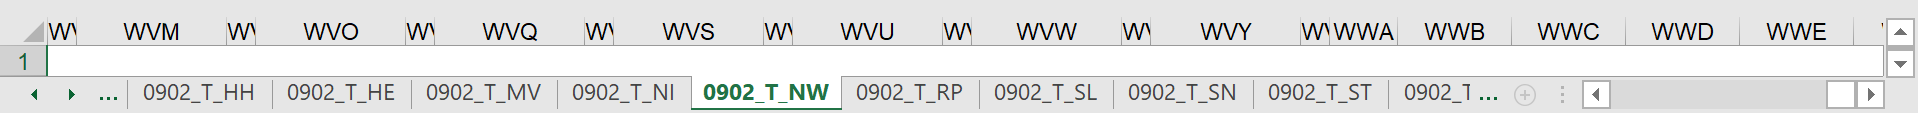
\includegraphics[width=\linewidth]{images/excel_shrink/cols/col_w2.png}
  \caption{Excessive Column Definitions in a Worksheet}
  \label{fig:col_w}
\end{figure}%

Columns \texttt{WWA} and the partially visible \texttt{WWB} correspond to the 16,147th and 16,148th columns, respectively. It seems improbable that an original worksheet would require the utilization of such an extensive number of columns. Further research is required to determine how such patterns emerge in \textit{Excel} files.

The last visible columns in Figure~\ref{fig:col_w} are shown in Listing~\ref{lst:columnsFoerderprogrammeEnd}. The first column \texttt{min="16146" max="16146"} has a fixed width of \texttt{2.21875} and refers to column \texttt{WVZ}, which is visible as the column immediately to the left of \texttt{WWA} but is too narrow to display more than the letter \texttt{W}. The second column \texttt{min="16147" max="16147"} defines column \texttt{WWA} with a width of \texttt{5.21875}. The final definition \texttt{min="16148" max="16384"} covers a larger range from column \texttt{16148} to \texttt{16384}, corresponding to columns \texttt{WWB} through \texttt{XFD} (the last column in \textit{Excel}). This explains why scrolling all the way to the right via the scrollbar lands on column \texttt{WWB}. The penultimate definition specifies where the data range ends, thereby also defining where the scrollable range ends, and the final definition simply assigns a default width to all remaining columns. Surprisingly, these column definitions extend all the way to \textit{Excel}'s maximum limit of 16,384 columns. We have no explanation for why these user-defined column widths appear up to just before the maximum allowable column, but not exactly at it.

To delete these columns, the following steps must be taken:
\begin{enumerate}
  \item Identify the actual right boundary of the data range and cell formats.
  \item Determine the first redundant column definition and save the \texttt{min} value to use it later.
  \item Delete all redundant column definitions except for the last one.
  \item Overwrite the \texttt{min} value of the last column definition with the saved value of the first redundant column definition.
\end{enumerate}

\begin{lstlisting}[caption={Final column definitions in the worksheet}, label={lst:columnsFoerderprogrammeEnd}, firstnumber={2414}, numbersep={-15pt}]
  <col min="16146" max="16146" width="2.21875" style="39" customWidth="1" />
  <col min="16147" max="16147" width="5.21875" style="39" customWidth="1" />
  <col min="16148" max="16384" width="8.77734375" style="39" customWidth="1" />
</cols>
\end{lstlisting}

Following these steps is crucial. We experimented with merely deleting the excess columns without ensuring that the last column definition extended to the final possible column (16,384), but this caused \textit{Excel} to mark these worksheets as corrupted and perform certain repairs. Part of these changes included altering the default row height, resulting in some worksheets appearing visually altered, as shown in Figures~\ref{fig:changed_default_row_height_before} and~\ref{fig:changed_default_row_height_after}. On the left is the original, and on the right is the repaired version by \textit{Excel}. For instance, row \texttt{6} has changed in height due to the repair, causing visible shifts in the worksheet. Correctly deleting column definitions while ensuring the last column definition extends to the column limit of 16,384 prevents this error.

\begin{figure}[ht]
  \centering
  \begin{subfigure}[b]{0.48\linewidth}
    \centering
    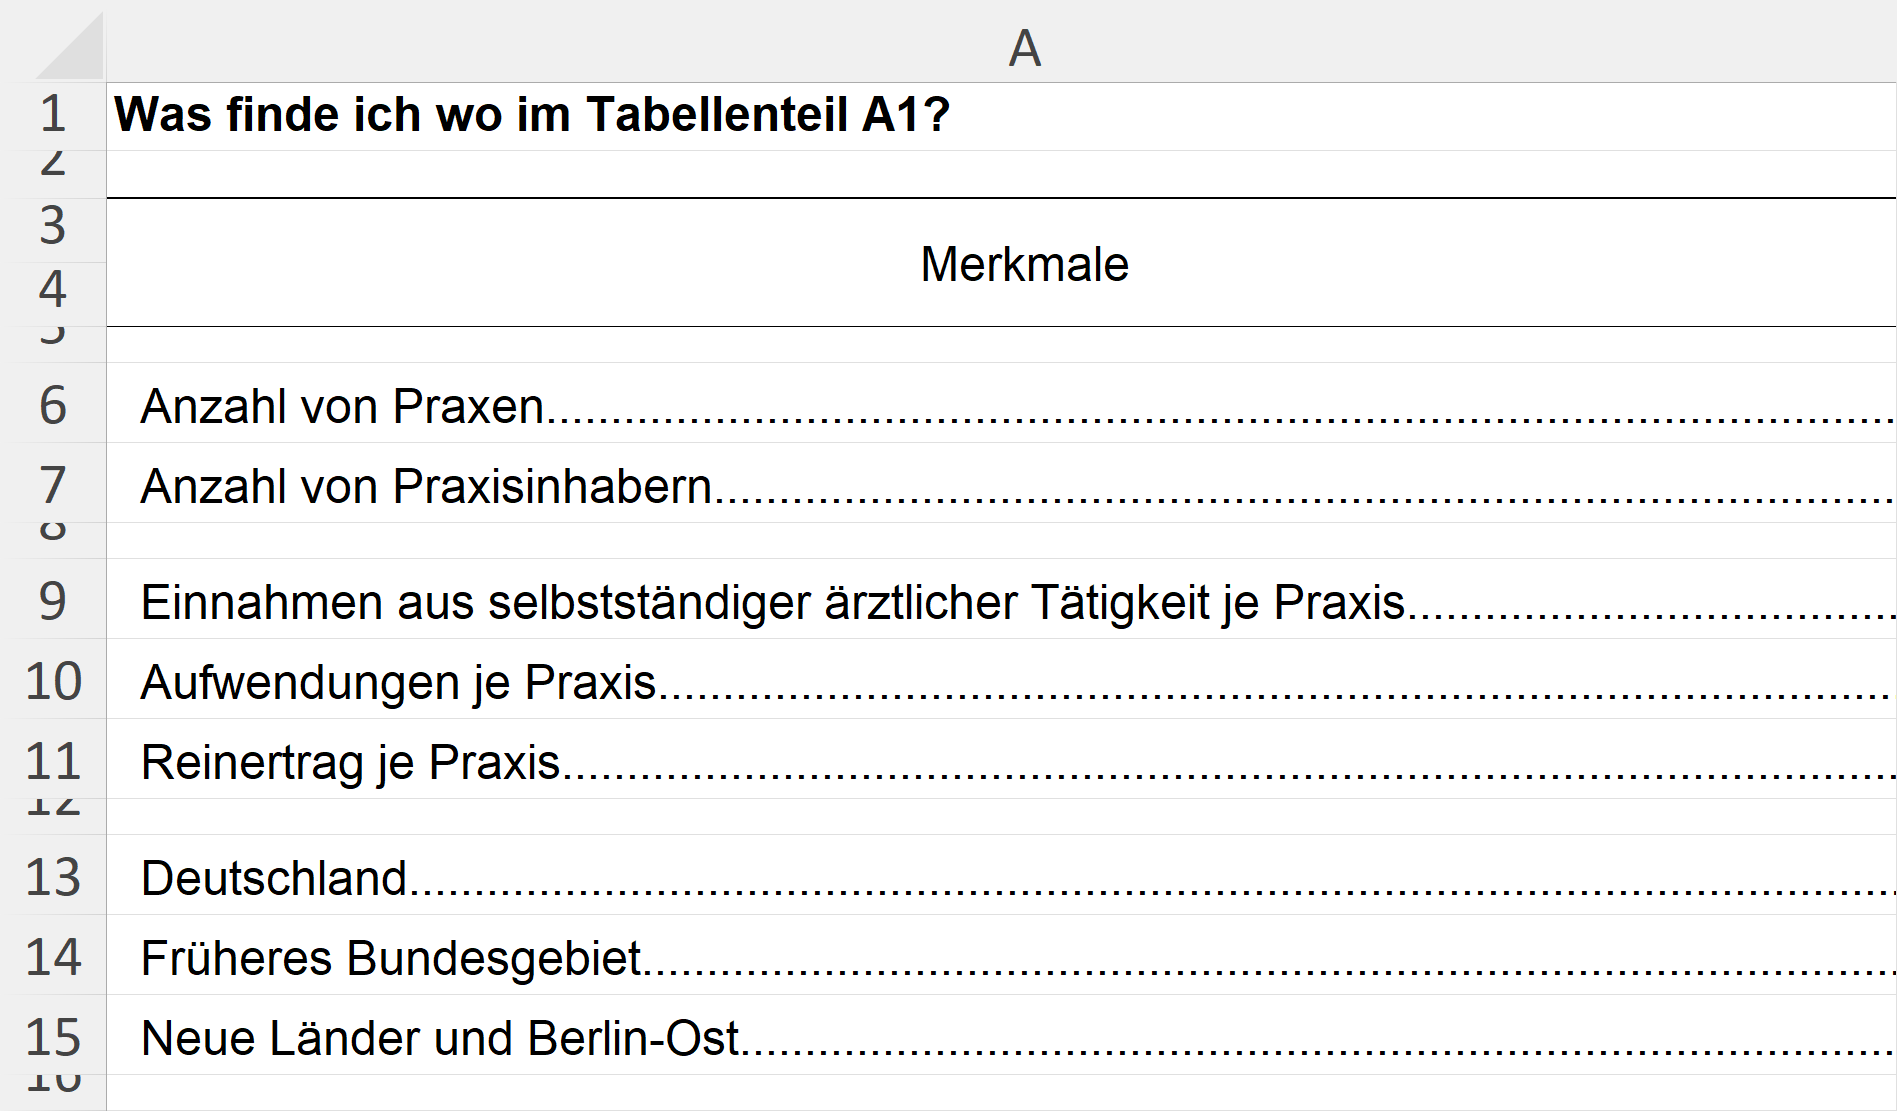
\includegraphics[width=\textwidth]{images/excel_shrink/changed_default_row_height/changed_default_row_height_before2.png}
    \caption{Original worksheet before repair}
    \label{fig:changed_default_row_height_before}
  \end{subfigure}
  \hspace{0.01\linewidth} % Space between images 
  \begin{subfigure}[b]{0.48\linewidth}
    \centering
    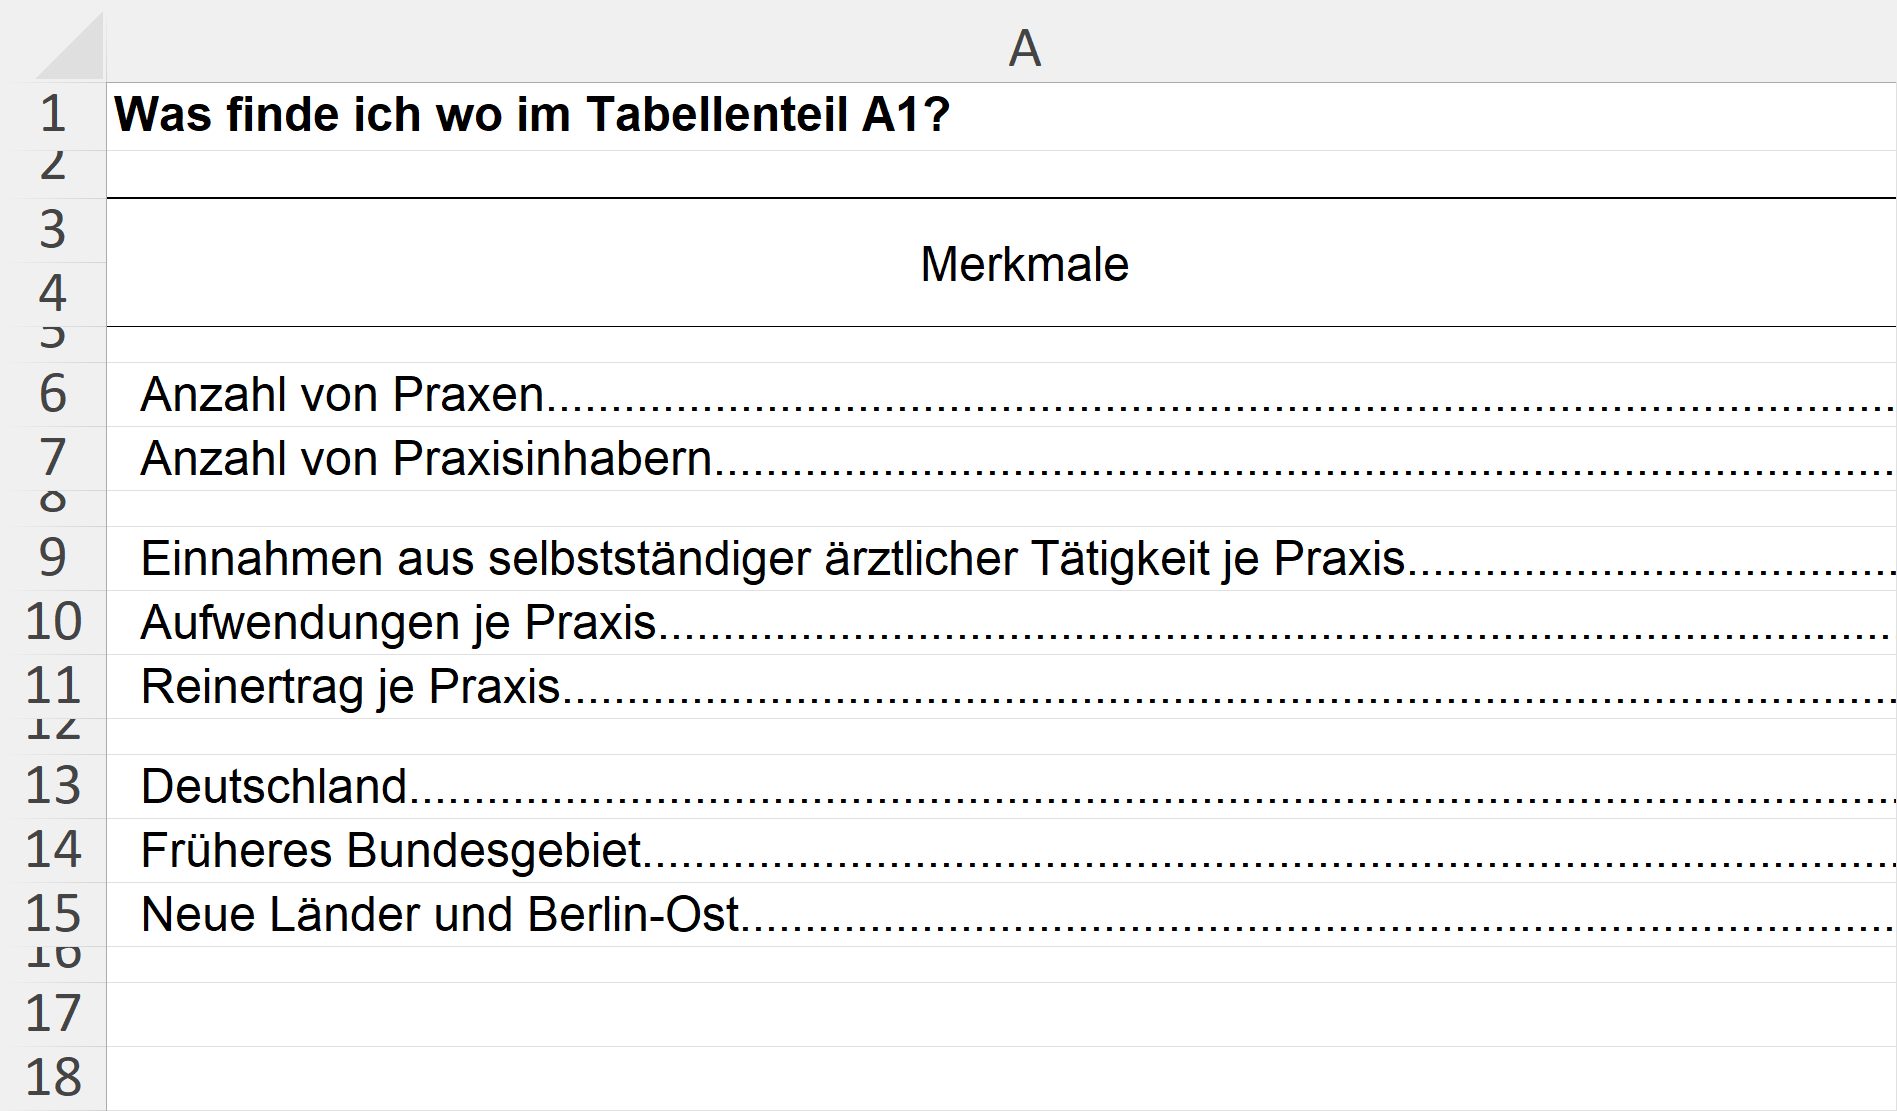
\includegraphics[width=\textwidth]{images/excel_shrink/changed_default_row_height/changed_default_row_height_after2.png}
    \caption{Worksheet after repair by \textit{Excel}}
    \label{fig:changed_default_row_height_after}
  \end{subfigure}
  \caption{Visual differences due to changes in default row height}
  \label{fig:changed_default_row_height}
\end{figure}

\subsubsection{Hidden Columns}

Removing columns is not recommended if there are hidden columns. In spreadsheets like \textit{Excel}, cells define only where text begins. If the text is longer than the cell, it typically extends over adjacent cells unless those cells also contain text. Some worksheets rely on the assumption that text will overflow into adjacent cells, causing the range of actually used cells to span multiple columns. In such cases, it's important not to delete columns outside the range of cells with values. Doing so could shift hidden columns to the next position, causing text from previous cells to overflow into them. This is depicted in Figures~\ref{fig:hidden_columns_before} and~\ref{fig:hidden_columns_after}. Since the texts are only defined in columns \texttt{A} and \texttt{B}, all cells from column \texttt{C} onwards are outside the range of cells with values and are thus considered for deletion. However, column \texttt{C} is already hidden, causing the texts to be cut off.

When \textit{Excel Shrink} detects hidden columns, it avoids removing them to ensure that the worksheet's visual representation is not altered.

\begin{figure}[ht]
  \centering
  \begin{subfigure}[b]{0.48\linewidth}
    \centering
    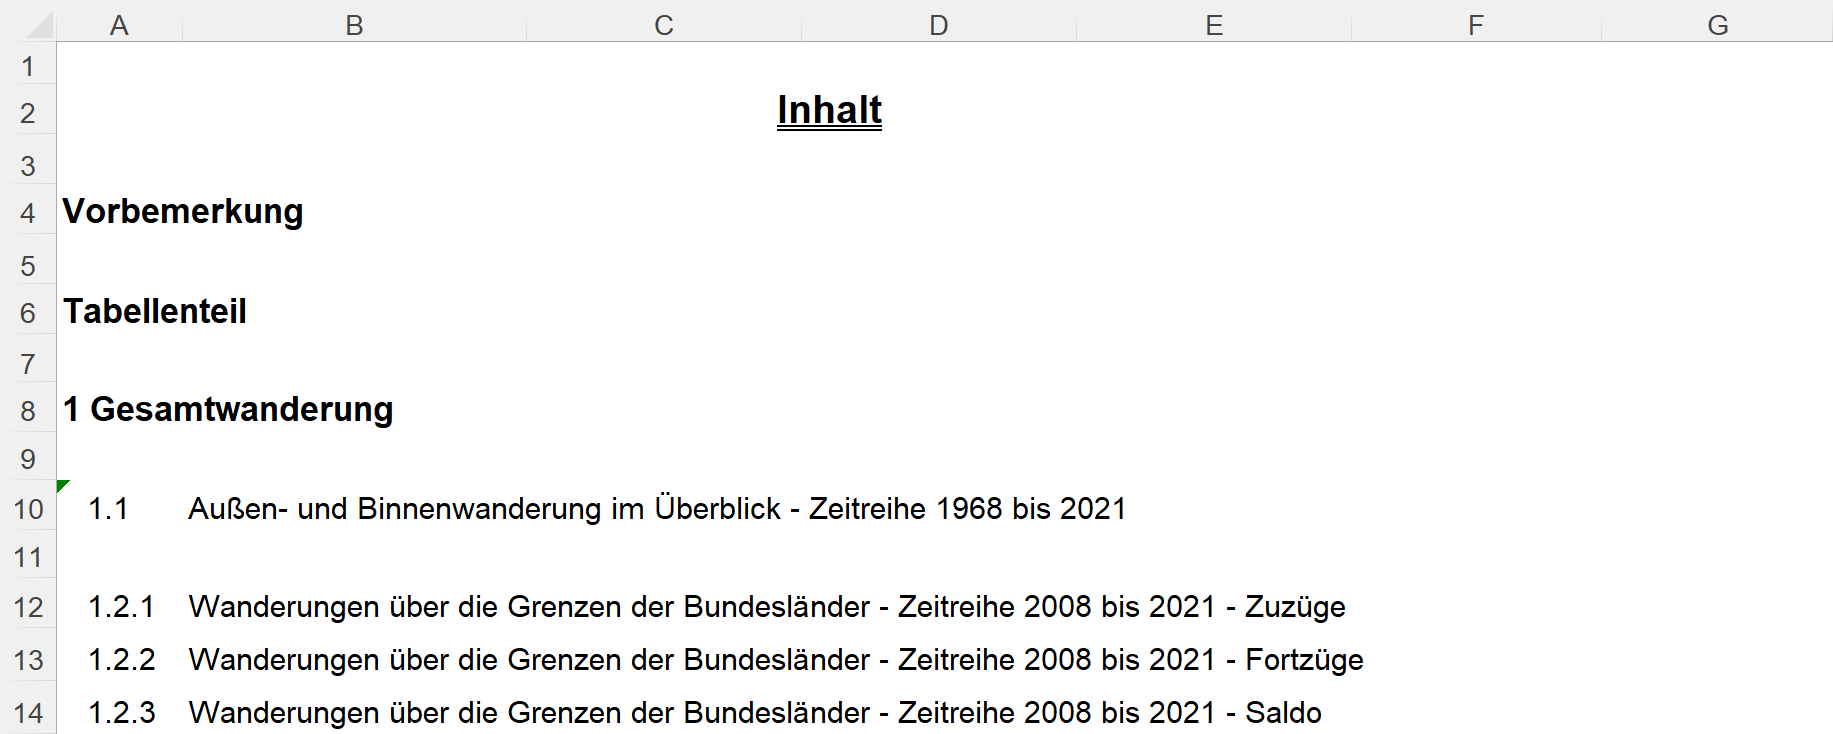
\includegraphics[width=\textwidth]{images/excel_shrink/hidden_columns/before2.png}
    \caption{Worksheet before column deletion}
    \label{fig:hidden_columns_before}
  \end{subfigure}
  \hspace{0.01\linewidth} % Space between images 
  \begin{subfigure}[b]{0.48\linewidth}
    \centering
    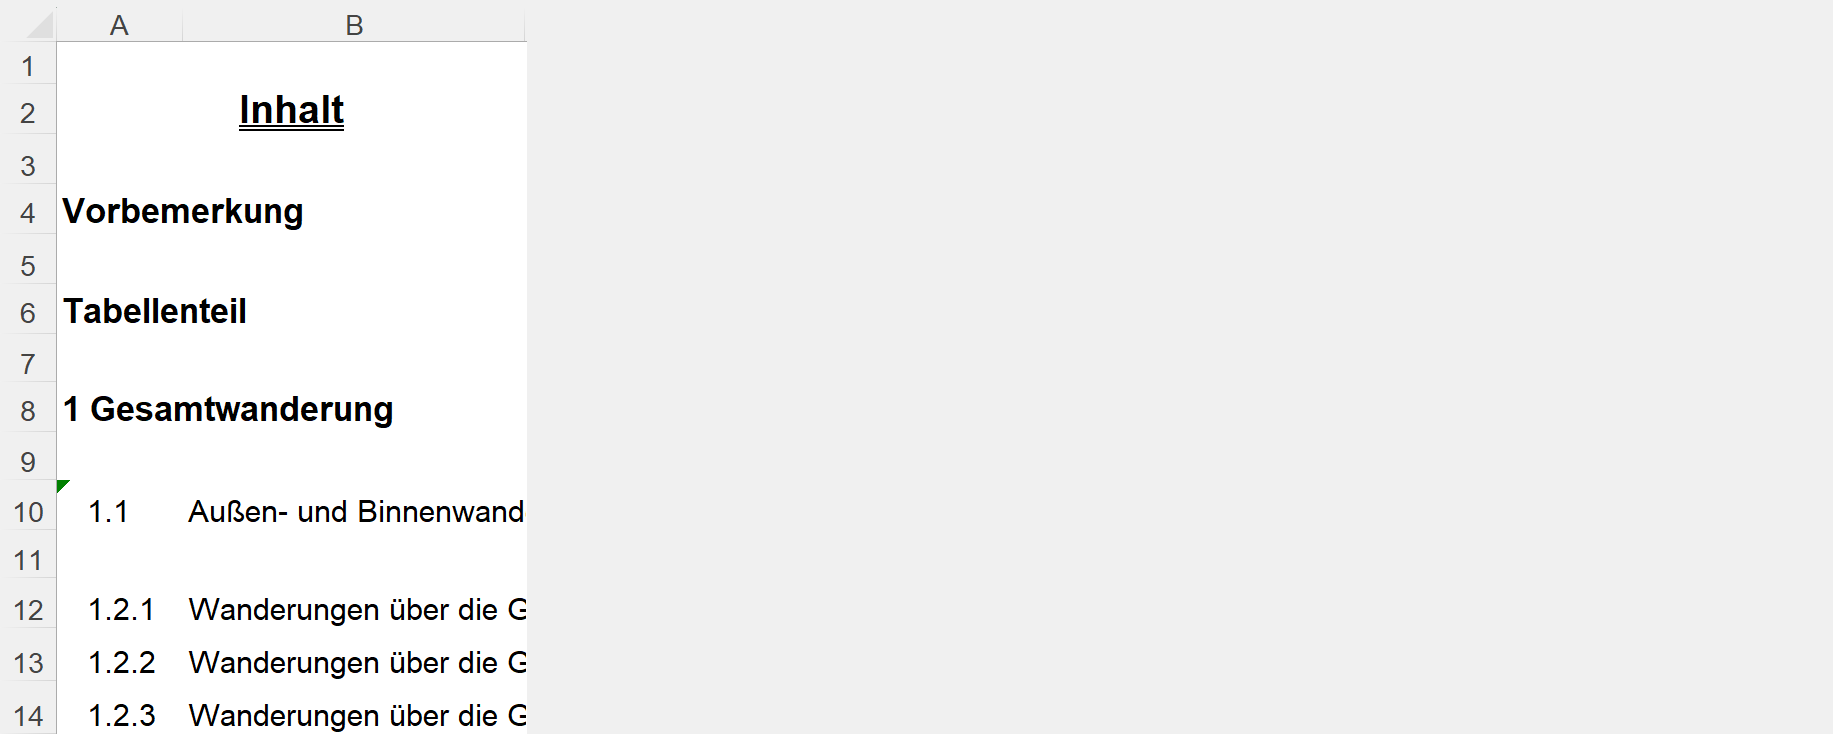
\includegraphics[width=\textwidth]{images/excel_shrink/hidden_columns/after2.png}
    \caption{Worksheet after column deletion}
    \label{fig:hidden_columns_after}
  \end{subfigure}
  \caption{Effect of deleting columns when hidden columns are present}
  \label{fig:hidden_columns}
\end{figure}

\subsection{Deletion of Empty Cells}

Some of the worksheets we examined contained vast numbers of cells without any content. The most extreme case was a worksheet with 8,141 cells containing values and 5,237,075 cells without values, meaning that only 0.15\% of the stored cells actually had a value~\cite[Sheet: \texttt{csv-71717-25}]{destatis2023Rechnungsergebnisse}. Listing~\ref{lst:cellsCsv7171725End} shows the last row of this worksheet.

\begin{lstlisting}[caption={The last row in the worksheet csv-71717-25}, label={lst:cellsCsv7171725End}]
  <row r="1048576" spans="3:7" ht="12.75" customHeight="1">
    <c r="C1048576" s="538"/>
    <c r="D1048576" s="537"/>
    <c r="E1048576" s="537"/>
    <c r="F1048576" s="537"/>
    <c r="G1048576" s="541"/>
  </row>
</sheetData>
\end{lstlisting}

Unlike the whitespaces, these cells now contain no value and therefore do not need to be cross-referenced with the sharedStrings file. However, it is possible that such empty cells may have a background color assigned, as is the case with some cover sheets used for page design or for highlighting table headers. Additionally, these cells might have borders applied.

To determine this, one must examine the \texttt{s} attribute, which stands for the style index applied to the cell. The values \texttt{s="538"}, \texttt{s="537"}, and \texttt{s="541"} correspond to indices in a lookup table where all cell styles are stored. The styles matching these style indices can be found in the \texttt{xl/styles.xml} file. The relevant excerpts are shown in Listing~\ref{lst:cellXfsCsv7171725}.

\begin{lstlisting}[caption={Cell styles in styles.xml for csv-71717-25}, label={lst:cellXfsCsv7171725}]
<cellXfs count="778">
  <!--538-->
  <xf numFmtId="0" fontId="0" fillId="0" borderId="0" xfId="0"/>
  <!--539-->
  <xf numFmtId="0" fontId="4" fillId="0" borderId="0" xfId="3" applyNumberFormat="1" applyFont="1"/>
  <!--542-->
  <xf numFmtId="0" fontId="1" fillId="0" borderId="0" xfId="1" applyNumberFormat="1" applyFont="1" applyAlignment="1">
    <alignment horizontal="right"/>
  </xf>
\end{lstlisting}

The XML structure within \texttt{<cellXfs>} contains formatting properties defined for cells in an \textit{Excel} file. Each \texttt{<xf>} element represents a formatting rule. Similar to the Shared Strings file, formatting rules are indexed based on their order in the list, starting with the first at 0, the second at 1, and so on. For the IDs \texttt{s="538"}, \texttt{s="537"}, and \texttt{s="541"}, one must look for the 539th, 538th, and 542nd elements in the list, respectively. The attributes control the cell's appearance. The \texttt{numFmtId} attribute specifies the number format used for the cell, while \texttt{fontId} describes the font ID. \texttt{fillId} refers to the fill color, and \texttt{borderId} defines the border properties. The \texttt{xfId} references a format template from which the cell inherits properties. The attributes \texttt{applyNumberFormat}, \texttt{applyFont}, and \texttt{applyAlignment} indicate whether the corresponding number format, font, and text alignment are applied to the cell. If the \texttt{alignment} element is present, it specifies the text alignment within the cell, such as right alignment. This structure defines the formatting rules used for the display and layout of the cell contents.

Inspection of these styles reveals that these cells only apply styles that are not visible for empty cells. They use different fonts, and cell \texttt{G1048576} is additionally right-aligned. Therefore, all these cells are redundant and can be deleted accordingly.

Another case arises when the formatting rules include borders. If such cells are simply deleted, as occurred in previous versions of our script, issues arise, as seen in Figure~\ref{fig:cell_borders_row_height}~\cite[Sheet: \texttt{2\_(1)}]{destatis2022Verkehrsunfaelle}. In Figure~\ref{fig:cell_borders_row_height_original}, all borders around the cells in the table header are visible. In Figure~\ref{fig:cell_borders_row_height_fail}, only the borders adjacent to cells with content remain visible. For example, the border between cells \texttt{A2} and \texttt{A3} is missing.

\begin{figure}[ht]
  \centering
  \begin{subfigure}[b]{0.48\linewidth}
    \centering
    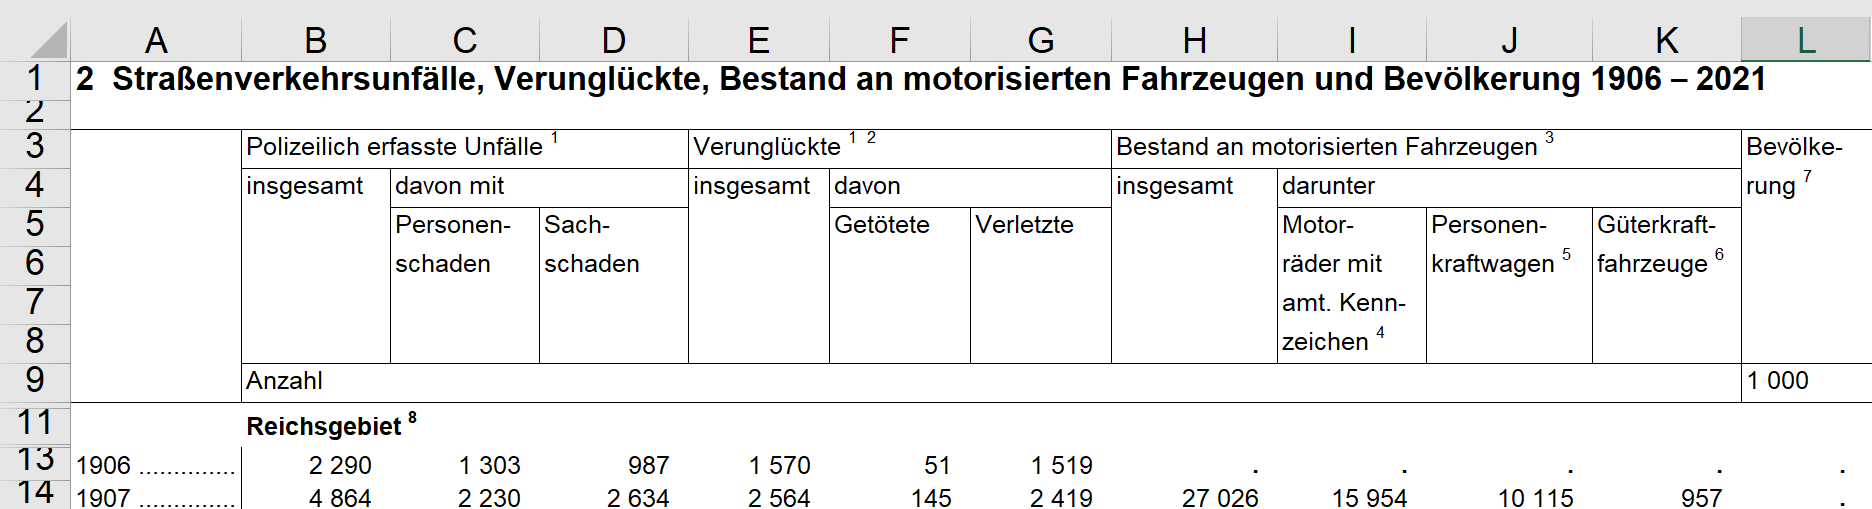
\includegraphics[width=\textwidth]{images/excel_shrink/borders/borders_original2.png}
    \caption{Original version with correct cell borders and spacing}
    \label{fig:cell_borders_row_height_original}
  \end{subfigure}
  \hspace{0.01\linewidth} % Space between images 
  \begin{subfigure}[b]{0.48\linewidth}
    \centering
    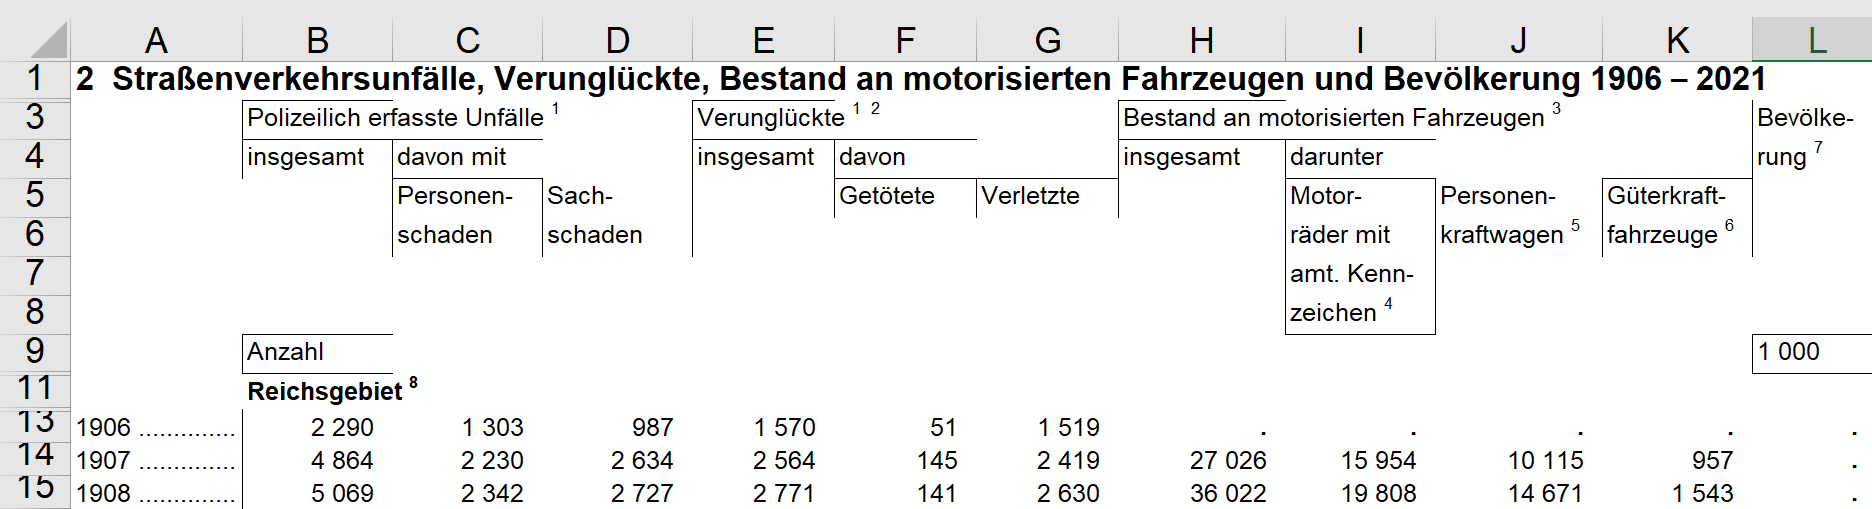
\includegraphics[width=\textwidth]{images/excel_shrink/borders/borders_fail2.png}
    \caption{Corrupted version with removed borders and spacing}
    \label{fig:cell_borders_row_height_fail}
  \end{subfigure}

  \caption{Erroneous removal of cells with borders and deletion of rows with custom heights}
  \label{fig:cell_borders_row_height}
\end{figure}

Cell \texttt{A2} appears in the XML as shown in Listing~\ref{lst:sheet-xml-a2}.

\begin{lstlisting}[caption={Cell A2 in sheet7.xml}, label={lst:sheet-xml-a2}, firstnumber=48, numbersep={-7pt}]
<c r="A2" s="577"/>
\end{lstlisting}

Here, the style ID is \texttt{s="577"}. It defines the underlying cell formatting, which in turn includes the ID for the border definition.

In the \texttt{styles.xml} file under the \texttt{<cellXfs>} node, we search for the \texttt{<xf>} node with ID \texttt{577}, which corresponds to the 578th \texttt{<xf>} node. This is shown in Listing~\ref{lst:style-xml-xf-577}.

\begin{lstlisting}[caption={Style with implicit ID 577 in styles.xml}, label={lst:style-xml-xf-577}, firstnumber=378]
<xf numFmtId="0" fontId="8" fillId="2" borderId="5" xfId="0" applyFont="1" applyFill="1" applyBorder="1" applyAlignment="1"/>
\end{lstlisting}

This \texttt{<xf>} node has the \texttt{borderId} attribute set to index \texttt{5}. Similar to cell styles, this index indicates that the 6th \texttt{<border>} node within the same \texttt{styles.xml} file is referenced.

Listing~\ref{lst:style-xml-border-5} shows the 6th \texttt{<border>} node with implicit ID 5.

\begin{lstlisting}[caption={Border node with implicit ID 5 in styles.xml}, label={lst:style-xml-border-5}, firstnumber=171]
<borders count="12">
  <!-- ... -->
  <border>
    <left/>
    <right/>
    <top/>
    <bottom style="thin">
      <color indexed="64"/>
    </bottom>
    <diagonal/>
  </border>
\end{lstlisting}

Each \texttt{<border>} node contains the child nodes \texttt{left}, \texttt{right}, \texttt{top}, \texttt{bottom}, and \texttt{diagonal}. If these nodes lack attributes or child nodes, it means that the cell has no border. In this case, the \texttt{bottom} node has the attribute \texttt{style} set to "thin" and includes the \texttt{color} node with the attribute \texttt{indexed="64"}, indicating that the cell has a thin black line at the bottom. Cells identified as having borders must not be deleted. Only cells that have neither content nor borders (i.e., their border nodes lack attributes indicating border presence) may be safely deleted.

\subsection{Inverted Fill}

During the development of \textit{Excel Shrink}, we made an interesting discovery. We found cells that had no content and no border but a fill definition that specified no fill should be applied. As a result, these cell definitions were deleted, and the cells turned red. We discovered that the entire row containing the cell had a red fill applied, and each cell within that row had a definition specifying that no fill should be applied to override the red fill color. As a user, one does not have any means to identify this by looking at the sheet. All the visible cells had the overridden fill color, and the rest of the cells were hidden behind hidden columns. Only after unhiding those columns did the issue become evident. Situations like these make preserving the visual appearance especially difficult.

We cannot simply decide to delete all cells that have a style applied that tells the cell to apply no fill because such a scenario might be useful in some situations. For example, if the whole row or column is intended to have a certain style and only some cells should apply no style as an exception to the rule. At the same time, in some scenarios, this might not be intended. The file becomes exceptionally large because some rows inadvertently have a style applied, and all cells in those rows up to the limit of possible columns define that this style should be overridden by no style.

To reduce the file size while preventing such changes to the display, we proceed as follows. First, we determine the style of the column and the row in which the cell is located. If either the column or row has a background color defined, we check whether the cell defines the same background color. In this case, we delete the cell. If the background color information of the cell differs from that of the column or row, we retain the cell. The same applies analogously to borders. If the column or row defines a border, we check whether the cell defines the same border. In this case, we delete the cell. If the border information of the cell differs from that of the column or row, we retain the cell.
\section{Deletion of Empty Rows}

Similar to cells without content but with visible formatting, rows may contain no defined cells but still have a defined height. Such rows must not be deleted because their height can affect the worksheet's layout. If such a row is deleted, an issue occurs as depicted in Figure~\ref{fig:cell_borders_row_height_fail} compared to the original in Figure~\ref{fig:cell_borders_row_height_original}. The spacing between the header and the table shrinks because the intermediate row, which served as spacing between the header and the table, is deleted, and the default row height for the worksheet is applied, which is smaller than the custom height of the row. This row is shown in Listing~\ref{lst:rowWithCustomHeight}.

\begin{lstlisting}[caption={Row with custom height}, numbersep={-7pt}, label={lst:rowWithCustomHeight}]
  <row r="2" spans="1:12" ht="8.25" customHeight="1">
\end{lstlisting}

The attribute \texttt{customHeight} means that this row has been assigned a user-defined height, specified by the \texttt{ht} attribute: \texttt{8.25}. Therefore, this row must not be deleted. However, during our examination of the worksheets, we found many that contained an immense number of empty rows, which had defined heights.

In the most extreme case in our analysis, a worksheet contained 1,048,576 defined rows. Of these, only 94 rows had content, which corresponds to approximately 0.00896\% of the total rows~\cite[Sheet: \texttt{Tabelle 1.2.1}]{destatis2022Wanderungen}. The remaining 1,048,482 rows had a defined height but were outside the data range.



\begin{lstlisting}[caption={The last row in the worksheet}, label={lst:lastRow}]
<row r="1048576" ht="12.75" hidden="1" customHeight="1"/>
\end{lstlisting}
After the 96th row, which is the last one with content, there are 1,048,482 rows that are identical to the last row shown in Listing~\ref{lst:lastRow}, except for the \texttt{r} attribute.
These rows all have the same height and are hidden, as indicated by the \texttt{hidden="1"} attribute. Although they are not displayed to the user, they have a user-defined height of 12.75 units, which is why they are still stored in the file. Row 1,048,576 corresponds to the last row, which is the maximum number of rows allowed in \textit{Excel}. If \textit{Excel} allowed a higher number of rows, the wasted file storage would be significantly greater.

We cannot rely on a row simply not having a defined height to decide whether it can be deleted. However, we also cannot simply delete rows that have a user-defined height, as they may be important for the worksheet's layout. Therefore, we must find another method to identify empty rows that can be safely deleted.

To ensure that deleting empty rows does not alter the worksheet's visual representation, we adopt a strategy similar to that used for removing columns. First, we determine the actual range where values, background colors, or borders are defined. Then, we iterate through all empty rows and delete them only if they lie outside this range. This approach allows us to significantly reduce the file size of some worksheets without altering their content or appearance.

\subsection{Deletion of Redundant Print Areas and Print Titles}
 
Excel allows users to define the area of a worksheet that should be printed on paper. This area can be manually defined or automatically set by \textit{Excel}. In both cases, this area is stored in the \texttt{workbook.xml} file under the \texttt{<definedNames>} node~\cite{microsoft2024workbook}. Typically, this area is labeled as \texttt{\_xlnm.Print\_Area} and \texttt{\_xlnm.Print\_Titles}. However, these areas and titles are often also stored under the names \texttt{Print\_Area} and \texttt{Print\_Titles}. When \textit{Excel} opens the file, it renames the entries \texttt{Print\_Area} and \texttt{Print\_Titles} to \texttt{\_xlnm.Print\_Area} and \texttt{\_xlnm.Print\_Titles}, respectively. This process creates a problem when there is already a \textit{Defined Name} for the same worksheet with both \texttt{Print\_Area} and \texttt{\_xlnm.Print\_Area}, as seen in Listing~\ref{lst:PrintAreaRedundancy}\cite[\texttt{xl/workbook.xml}]{destatis2022Wanderungen}.

\begin{lstlisting}[caption={Redundant Print Area entries}, label={lst:PrintAreaRedundancy}, firstnumber=171]
<definedName name="_xlnm.Print_Area" localSheetId="12">'Tabelle 2.1.1'!$A$1:$N$64748</definedName>
<!-- ... -->
<definedName name="Print_Area" localSheetId="12">'Tabelle 2.1.1'!$A$1:$N$93</definedName>
\end{lstlisting}

The same applies to \texttt{Print\_Titles} and \texttt{\_xlnm.Print\_Titles}. In this case, the entries cannot be renamed because it would lead to redundant entries. Instead, \textit{Excel} presents a dialog to the user upon opening the file, asking the user to select a new name for the \textit{Defined Name}.

If the first entry is renamed and the user clicks OK, the dialog reappears for the next entry. This process repeats until all redundant entries for both \texttt{Print\_Area} and \texttt{Print\_Titles} are renamed. However, the user cannot simply enter the same name repeatedly to shorten this process, as \textit{Excel} will prevent the same name from being used twice for different \textit{Defined Names} on the same worksheet. Dieser Dialog verhinder auch, die Dateien mit VBA automatisiert zu öffnen um mittels des Plugins Inquire oder dem Excel Performance Tab die Dateigröße zu verringer, da beim öffnen jeder Datei über VBA dieser Dialog auftaucht und die automatisierung anhält.  

In the files we examined, there were up to 60 redundant \texttt{Print\_Area} and 55 \texttt{Print\_Titles} entries. Renaming these entries offers no advantage to the user, as these entries are only stored in the \textit{Defined Names} accessible via \textit{Excel}'s \texttt{Formulas}~$\rightarrow$~\texttt{Name Manager}. Users might think that they are repairing the \textit{Print Areas} or \texttt{Print Titles} by entering those new names, but this is not the case because those \textit{Print Areas} and \texttt{Print Titles} are already migrated correctly. In reality, the user only renames redundant \textit{Defined Names}. To simplify the analysis and spare users the need to manually rename redundant entries, \textit{Excel Shrink} was extended to automatically remove redundant entries.


\subsection{Reporting Reduction Results}

To provide a breakdown of how many bytes were saved by deleting whitespaces, empty cells, columns, and rows, we compare the file size before and after each reduction step. For this purpose, we calculate the size of the worksheet by converting the XML structure into a string, as it would be stored in the file, and compute the length of this string. We then perform a reduction step and again calculate the length of the new string to determine the difference caused by the reduction. Finally, we calculate the percentage reduction relative to the original size. These results are saved in a CSV table.~\cite{excel_shrink_results_csv}



 









\begin{figure*}
  \centering
  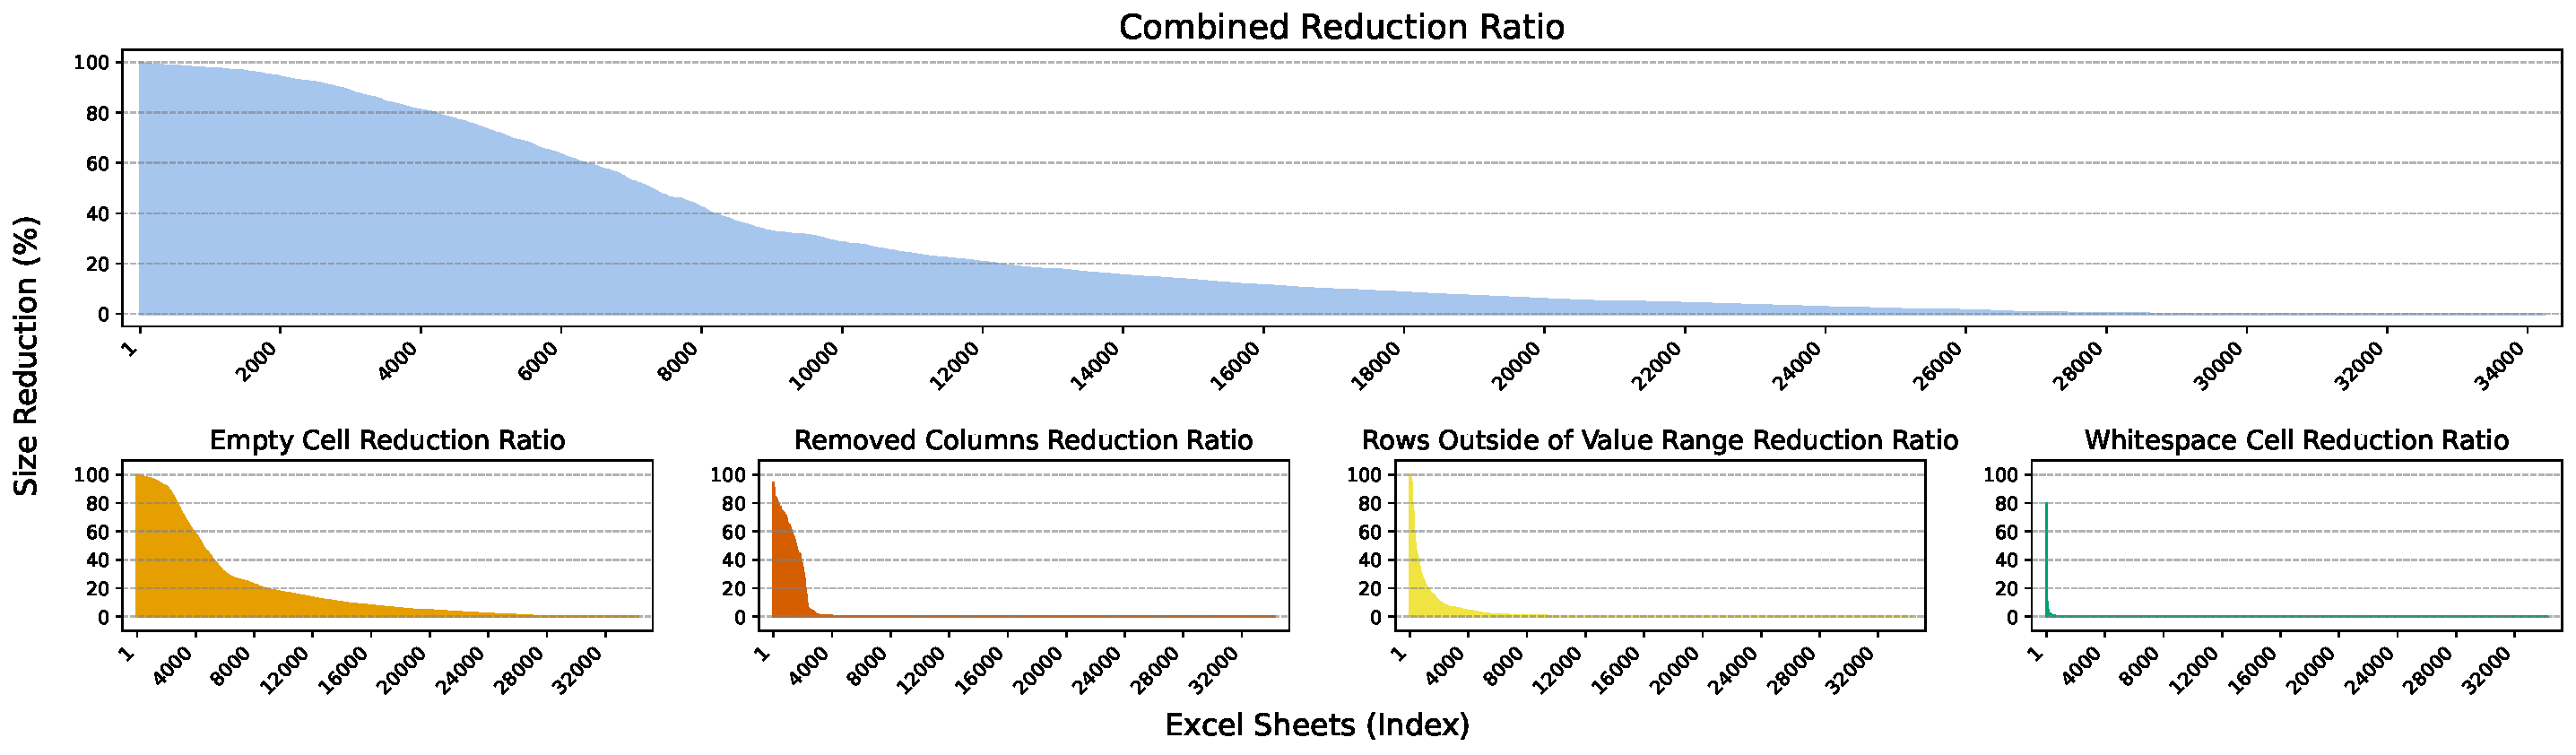
\includegraphics[width=\textwidth]{images/charts/combined_chart_distribution_of_size_reduction.pdf}
  \caption{Distribution of Size Reduction Percentages for Excel Sheets}
  \label{fig:size-reduction-chart}
\end{figure*}

  
\section{Evaluation}

In this evaluation, we processed all \textit{Excel} files obtained from the German Federal Statistical Office (\textit{Destatis})~\cite{original_destatis_xlsx_files,shrinked_destatis_xlsx_files}. The complete details of how these files were acquired through a custom web scraping approach can be found in Appendix~\ref{sec:scraping_destatis}.

Our primary goal was to quantify the extent of data reduction achieved by \textit{Excel Shrink}, focusing on metrics such as overall size reduction, removal of empty cells, elimination of whitespace cells, deletion of rows outside the value range, and the removal of unnecessary columns. Figure~\ref{fig:size-reduction-chart} presents the distribution of reduction rates (in percentage) for individual worksheets across all these categories. The chart shows that some worksheets experienced reductions approaching 100\% in file size. In particular, one worksheet exceeded a 99.99\% reduction, 16 worksheets surpassed 99.9\%, and 210 worksheets achieved reductions above 99\%. Across all worksheets, the average reduction rate was 25\%. Most of these gains were realized by removing rows that lay outside the range of actual data values.

To further assess the performance improvements enabled by \textit{Excel Shrink}, we identified the largest available \textit{Destatis} file.\footnote{The file reference can be found here: [LINK TO THE FILE].} Prior to processing, this file measured 85.2~MB in its compressed \textit{Excel} (.xlsx) format and expanded to 911~MB when uncompressed. After applying \textit{Excel Shrink}—a process that took approximately 935.5 seconds—the resulting compressed file size was reduced to 2.76~MB, with an uncompressed size of just 20.6~MB.

We then tested file opening times using the Dart \texttt{excel} package. Before shrinking, the first run took 794.7 seconds to open and read values from the file. On the second run, the process failed due to an out-of-memory exception. In contrast, after applying \textit{Excel Shrink}, we successfully ran the test 10 consecutive times without error. The median time to open the shrunk file and read values was 17.90 seconds, demonstrating a substantial performance improvement.

\subsection{Summary of Findings}

The evaluation demonstrates that the data reduction techniques employed by \textit{Excel Shrink} are highly effective in eliminating redundant, empty, or irrelevant data across a variety of \textit{Excel} worksheets. Significant reductions—exceeding 90\% in several cases—were achieved in sheets containing a high proportion of empty cells, or irrelevant rows and columns. These results highlight the robustness of our reduction methods in processing diverse data formats and structures.

Moreover, the analysis underscores the importance of addressing different reduction factors independently, as their impact on file size varied. While empty cell removal provided substantial reductions in certain worksheets, others benefited more from the removal of rows or columns. Notably, whitespace removal had a smaller overall impact.

\section{Experimental Setup}
\label{sec:experimental-setup}

To evaluate the behavior of \textit{Excel} regarding how the files are interpreted and saved, as well as to test the behavior of the \textit{Add-in} and the new \textit{Check Performance} feature, we tested with two distinct versions of \textit{Excel} from \textit{Microsoft Office}: \textit{Microsoft Office LTSC Professional Plus 2021} and \textit{Microsoft Excel for Microsoft 365 MSO (Version 2409 Build 16.0.18025.20030) 64-bit}. These versions were selected to evaluate compatibility and performance across different Excel environments.Our test machine was an \textit{Intel Core i7-4790K} quad-core CPU desktop machine running at 4.00~GHz with 16~GB of RAM.

\section{Conclusion}
\label{sec:conclusion}

We have presented \textit{Excel Shrink}, an open-source tool that significantly reduces the file sizes of \textit{Excel} sheets from \textit{Destatis} by eliminating unnecessary content. Our analysis identified common practices that lead to bloated \textit{Excel} files and demonstrated how targeted removal of redundant data can achieve reductions of up to 99.99\% without altering the spreadsheets' appearance.

Our tool outperforms existing solutions in both file size reduction and preservation of formatting. By making \textit{Excel Shrink} available to the community, we hope to facilitate more efficient data processing and analysis of large-scale \textit{Excel} datasets.

%\clearpage


\section{Old Background}


\subsection{Limitations of Existing Solutions}

Several proprietary tools and features, such as NXPowerLite Desktop, the Inquire Add-in, and the Excel Performance tab, attempt to mitigate file bloat. However, they suffer from notable shortcomings:

\begin{itemize}
    \item \textbf{Closed Source and Lack of Transparency:} Existing tools do not disclose their underlying methods, making it difficult to understand the root causes of bloat or to improve upon their techniques.
    \item \textbf{Incomplete Coverage:} They often fail to address all sources of unnecessary content. For example, redundant column definitions may remain uncorrected, leaving substantial portions of file bloat unresolved.
    \item \textbf{Visual Alterations:} Some solutions can significantly alter the spreadsheet’s original appearance, which is unacceptable for users who rely on specific formatting or corporate branding.
    \item \textbf{Limited Automation:} Due to the lack of batch processing or command-line interfaces, integrating these tools into automated workflows or pipelines (e.g., for cloud uploads or large-scale data processing) is challenging or impossible.
\end{itemize}

\subsection{Our Approach and Contributions}

Motivated by these gaps, we conducted a systematic investigation into the root causes of Excel file bloat, focusing on previously undocumented inefficiencies and the limitations of existing solutions. We then developed \textit{Excel Shrink}, an open-source tool designed to effectively reduce file sizes while preserving the spreadsheet’s visual appearance. Unlike proprietary offerings, \textit{Excel Shrink} provides a transparent, platform-independent solution that does not require Microsoft Excel itself. It can also be integrated into automated pipelines, enabling seamless batch processing and large-scale deployment. For those preferring a more user-friendly interface, we offer \textit{Excel Shrink UI}~\cite{excel-shrink-ui}, which eliminates the need for Python installation or command-line interactions.

Our contributions are as follows:

\begin{itemize}
    \item \textbf{Comprehensive Analysis:} We reveal the root causes of file bloat in Destatis Excel files, identifying previously undocumented issues such as unnecessary column definitions.
    \item \textbf{Critical Evaluation of Existing Tools:} We show why current proprietary solutions fail to fully resolve file bloat and how they may inadvertently alter the spreadsheet’s appearance.
    \item \textbf{Novel Open-Source Solution:} We introduce \textit{Excel Shrink}, which effectively addresses all identified causes of bloat, preserves visual formatting, supports automation, and is not tied to a specific operating system or to Microsoft Excel.
    \item \textbf{Empirical Validation:} We evaluate \textit{Excel Shrink} on a comprehensive set of Destatis Excel files, demonstrating that it can reduce file sizes by up to 99.99\% without compromising usability or appearance.
\end{itemize}

By thoroughly examining hidden redundancies and providing a transparent, open-source solution, our work fills a significant gap in spreadsheet optimization research and practice.


\section{Old Related Work}
\label{sec:related-work}

Several tools and techniques have been developed to reduce \textit{Excel} file bloat, including proprietary solutions such as \textit{NXPowerLite Desktop}, the \textit{Excel Inquire} Add-in, and the built-in \textit{Check Performance} feature in recent versions of \textit{Excel}. While these tools can alleviate certain issues, they also exhibit notable limitations.

\subsection{NXPowerLite Desktop}

\textit{NXPowerLite Desktop} is a commercial application primarily focused on compressing embedded images in \textit{Excel} files~\cite{neuxpower2024nxpowerlite}. Although it can remove some empty cells, it disregards other sources of file bloat such as cells containing only whitespace and redundant column definitions.

The tool offers limited batch functionality, allowing users to select and process multiple files simultaneously, but only up to a maximum of 20 files at once. Being closed-source, it does not provide a means to adjust this artificial limit, further motivating the need for a more flexible, open-source solution.

\subsection{Excel Inquire Add-in}

The \textit{Excel Inquire} Add-in, available only in \textit{Office Professional Plus} and \textit{Microsoft 365 Apps for Enterprise}, can remove some redundant content~\cite{o2014excel}. However, it lacks comprehensive batch processing capabilities because it requires manually opening each \textit{Excel} file before applying the add-in. This approach is impractical for large datasets.

\textit{Excel Inquire} ignores whitespace cells but can delete empty cell, column, and row definitions. Yet, in certain cases, a significant number of unnecessary elements remain. For example, consider a worksheet serving as a cover sheet, where only the first 77 rows are used and the remaining rows (78 to 65533) are hidden. Despite being hidden, all these rows and cells are defined in the XML structure, as shown in Listing~\ref{lst:row-65533}.

\begin{lstlisting}[caption={Row 65533 in sheetX.xml}, label={lst:row-65533}]
<row r="65533" spans="1:7" ht="0" hidden="1" customHeight="1">
  <c r="A65533" s="68" />
  <c r="B65533" s="68" />
  <c r="C65533" s="68" />
  <c r="D65533" s="68" />
  <c r="E65533" s="68" />
  <c r="F65533" s="68" />
  <c r="G65533" s="68" />
</row>
</sheetData>
\end{lstlisting}

When applying the \textit{Excel Inquire} Add-in to such worksheets, these hidden rows and cells remain. A dialog box reports that because the default row height is \texttt{0}, the tool cannot clean the sheet, causing the operation to be skipped entirely.
\subsection{Excel Check Performance}

The \textit{Check Performance} feature, introduced in \textit{Excel} for the Web and recent desktop versions, can achieve substantial file size reductions~\cite{shirolkar2022check,shirolkar2024make}. However, it often removes cells and rows that influence the spreadsheet’s layout and formatting, thereby altering its visual appearance. This is unacceptable in contexts where maintaining the original look and structure of the spreadsheet is essential.

Figure~\ref{fig:performance} illustrates how \textit{Check Performance} modifies a cover sheet by removing empty rows. While such modifications might be acceptable in some instances, they become problematic when these empty rows serve a functional purpose, such as aligning the layout for printing on A4 pages. In the example shown, the cells responsible for providing whitespace on the cover sheet (Figure~\ref{fig:performance_before}) are removed, as shown in Figure~\ref{fig:performance_after}~\cite{destatis2022Verkehrsunfaelle}.

\begin{figure}[ht]
  \centering
  \begin{subfigure}[b]{0.48\linewidth}
    \centering
    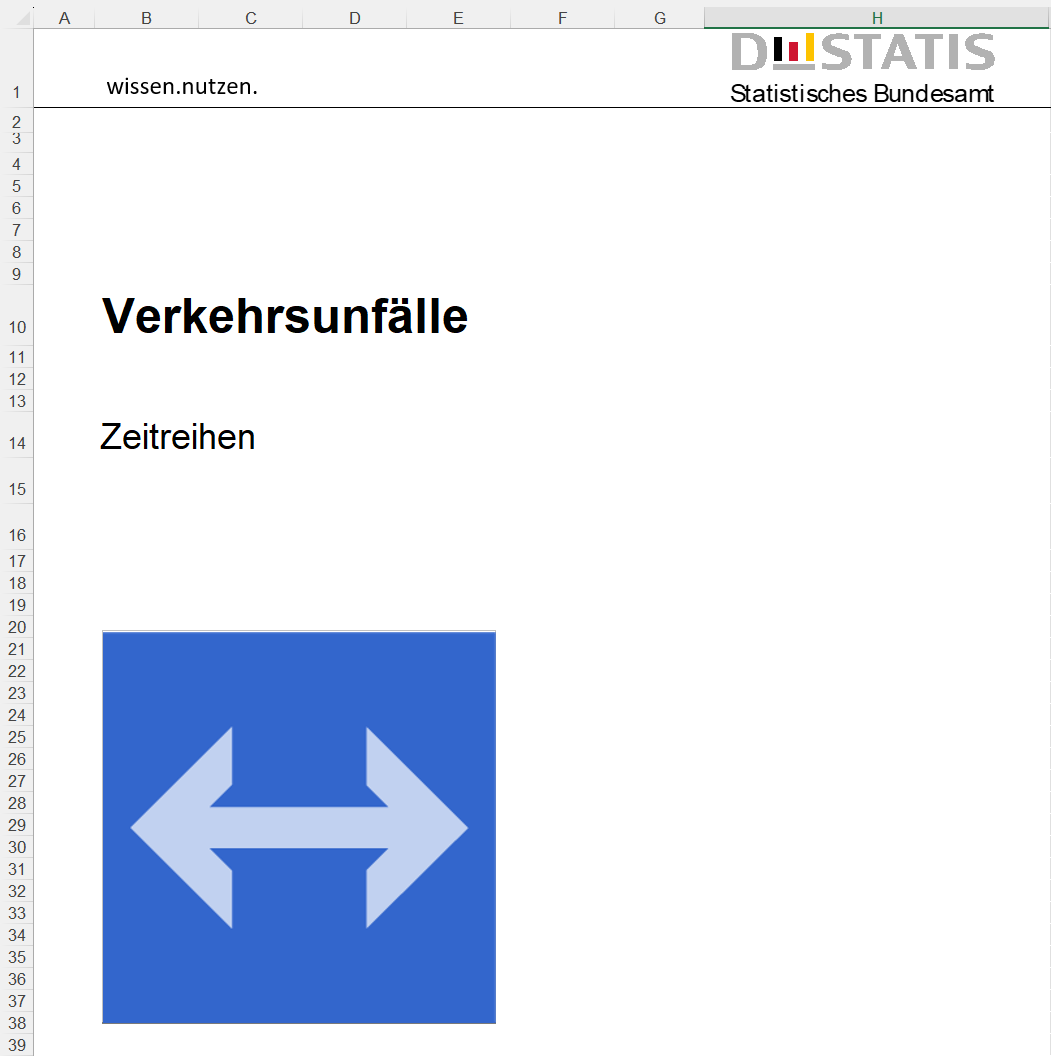
\includegraphics[width=\textwidth]{images/excel_shrink/related_work/performance/verkehrsunfaelle-performance.png}
    \caption{Before Applying Check Performance}
    \label{fig:performance_before}
  \end{subfigure}
  \hspace{0.01\linewidth} 
  \begin{subfigure}[b]{0.48\linewidth}
    \centering
    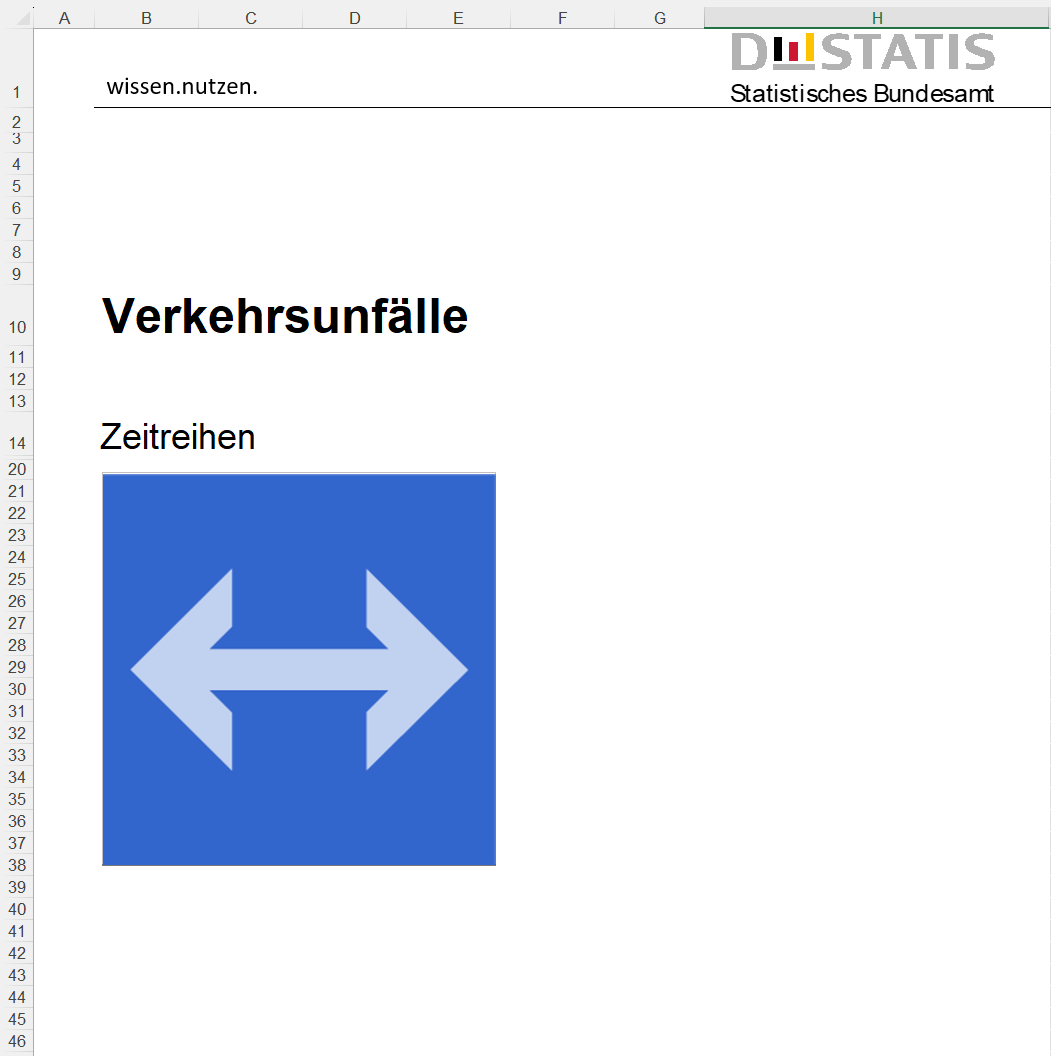
\includegraphics[width=\textwidth]{images/excel_shrink/related_work/performance/verkehrsunfaelle-performance_after.png}
    \caption{After Applying Check Performance}
    \label{fig:performance_after}
  \end{subfigure}
  \caption{Comparison of a Cover Sheet Before and After Applying Check Performance}
  \label{fig:performance}
\end{figure}

As another example, consider a form-like structure composed of several empty cells arranged to form a table, anticipating future data entry~\cite{destatis2023Rechnungsergebnisse}. \textit{Check Performance} removes all borders outside the active data region, resulting in the scenario shown in Figure~\ref{fig:table_no_table}, where the intended table layout is lost.

\begin{figure}[ht]
  \centering
  \begin{subfigure}[b]{0.48\linewidth}
    \centering
    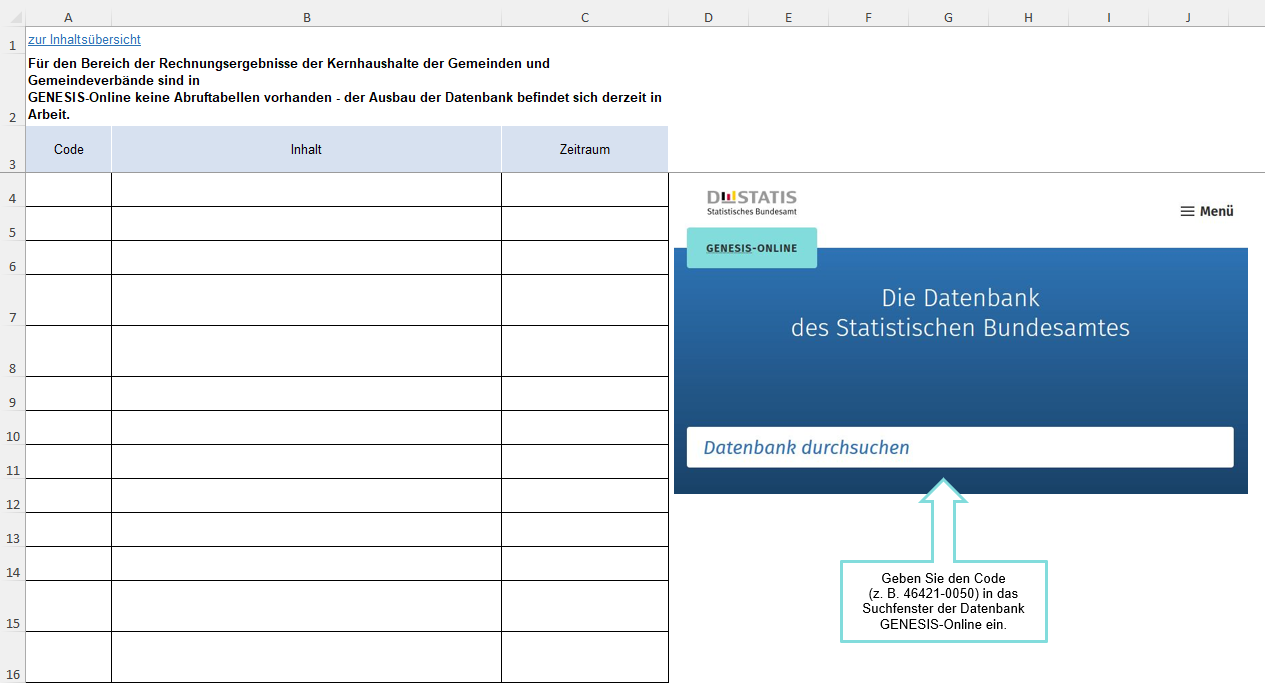
\includegraphics[width=\textwidth]{images/excel_shrink/related_work/performance/table2.png}
    \caption{Before Applying Check Performance}
    \label{fig:table}
  \end{subfigure}
  \hspace{0.01\linewidth} 
  \begin{subfigure}[b]{0.48\linewidth}
    \centering
    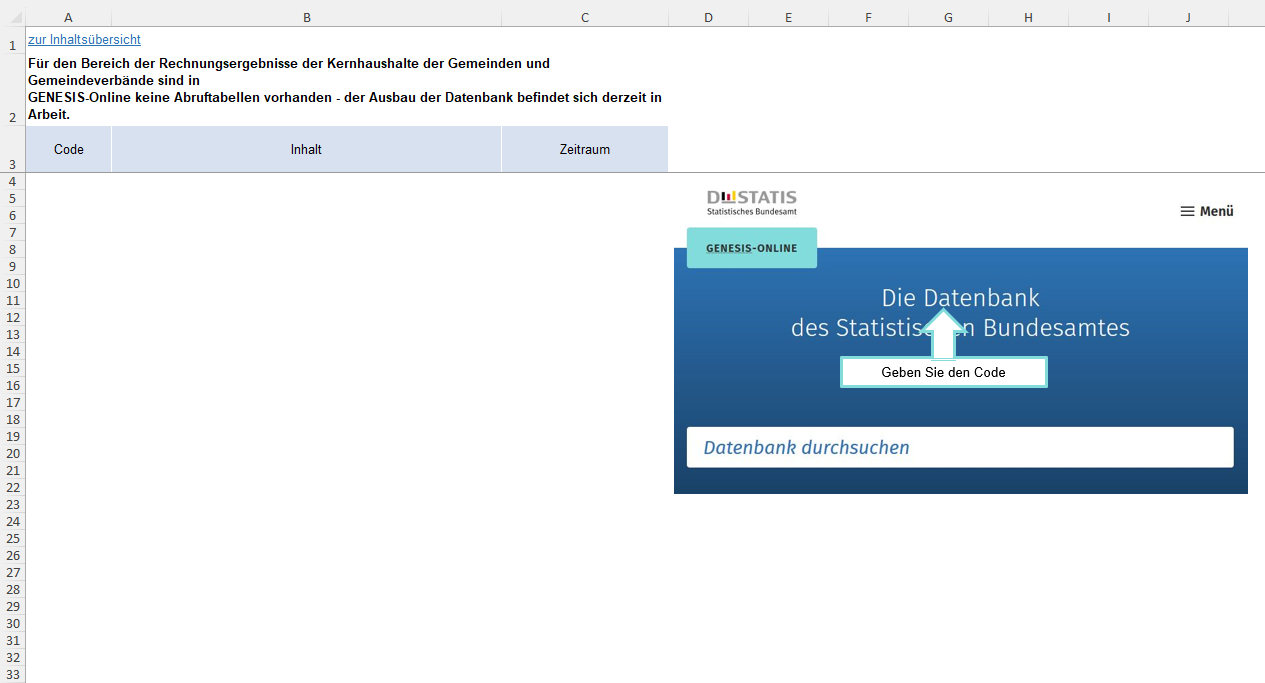
\includegraphics[width=\textwidth]{images/excel_shrink/related_work/performance/no_table2.png}
    \caption{After Applying Check Performance}
    \label{fig:no_table}
  \end{subfigure}
  \caption{Removal of Borders Defining an Empty Table Structure}
  \label{fig:table_no_table}
\end{figure}





\section{Scraping Destatis}
\label{sec:scraping_destatis}

The \textit{Destatis} website does not provide an API for searching publications, making it necessary to interact with the website directly. To automate this process, we developed a web scraper that searches for relevant publications while minimizing the number of requests to the server. The web scraping and downloading process is outlined in Algorithm~\ref{alg:web_scraping_caching}. The URL structure of the \textit{Destatis} website is as follows, with query parameters appended to the base path:

\begin{itemize}
  \item \url{/SiteGlobals/Forms/Suche/Expertensuche\_Formular.html}:

  This is the base path of the URL, which points to the expert search form on the \textit{Destatis} website. It serves as the primary endpoint where the search query is submitted.

  \item \url{templateQueryString=2000}:

  This query parameter specifies the search year. In this case, the search is focused on publications from the year 2000. By adjusting this value, different years can be searched.

  \item \url{gtp=474\_list\%253D2}:

  This parameter handles pagination. It points to a specific page of search results. The value \texttt{\%253D} is a doubly encoded sequence, where \texttt{\%253D} is the URL-encoded form of \texttt{\%3D}, which itself encodes the equal sign (\texttt{=}). After decoding twice, the query parameter becomes \texttt{gtp=474\_list=2}. The number after the second equal sign corresponds to the current page index in the pagination of the search results.


  \item \url{documentType\_=publication}:

  This parameter filters the results by the type of document. By setting this to \texttt{publication}, the search is limited to publications, where \textit{Excel} files are usually attached.

  \item \url{resultsPerPage=100}:

  This parameter determines how many results should be displayed per page. In this case, it is set to \texttt{100}, which is the maximum number of results that can be retrieved in a single page request.
\end{itemize}

Through extensive testing, we discovered that \textit{Excel} files are exclusively found in the ``Publication'' document type. By using the GET parameter \texttt{documentType\_=publication}, we were able to significantly narrow down our search results.

Initially, we assumed that searching for the term \texttt{xlsx} would identify all publications containing \textit{Excel} file attachments. However, this search only returned about 100 results, far fewer than the actual number of \textit{Excel} files available on the \textit{Destatis} website. Furthermore, there is no option to retrieve a complete list of all publications ever created. To overcome this, we refined our strategy by searching based on publication years. A publication should appear in the search results when queried by its publication year. Although this approach returns some irrelevant results---where the publication year might appear in the text or a file attachment---the number of requests is greatly reduced by caching and reusing links to the \textit{Excel} file attachments. This ensures that the same files are not downloaded multiple times.

The search results on the \textit{Destatis} website, like many others, are paginated, with the interface offering the ability to display 10, 20, or 30 entries per page. The number of results per page can be adjusted using the GET parameter \texttt{resultsPerPage=30}. While the interface does not provide an option for more than 30 results per page, we found that manually setting this parameter allowed us to request up to 100 results per page. Through testing, we confirmed that 100 is the maximum number of results that can be returned at once. We set the \texttt{resultsPerPage} parameter accordingly to reduce the number of requests further.

Once the results for a page are fetched by the web scraper, we simulate clicking the ``next page'' link to load subsequent results. The XPath expression \texttt{//a[@class='forward button']/@href} is used to identify the link using the CSS class \texttt{forward button}.
\begin{algorithm}
  \caption{Processing and Cleaning Excel Files in Place}
  \label{alg:process_xlsx_in_place}
  \begin{algorithmic}

    \STATE \textbf{Input:} 
    \STATE \quad \texttt{InP} $\leftarrow$ Excel file path
    \STATE \quad \texttt{OutP} $\leftarrow$ Output path
    \vspace{0.2cm}
    
    \STATE \texttt{InArc} $\leftarrow$ Open the ZIP archive \texttt{InP} for reading
    \STATE \texttt{OutArc} $\leftarrow$ Create a new ZIP archive for writing
    \STATE \texttt{ShStr} $\leftarrow$ Extract Shared strings  from \texttt{sharedStrings.xml}
    \STATE \texttt{Sty} $\leftarrow$ Extract Styles from \texttt{styles.xml}
    \STATE \texttt{SF} $\leftarrow$ List of all sheet XML files in \texttt{Arc}
    \STATE \texttt{NSF} $\leftarrow$ List of non-sheet files in \texttt{Arc}    \vspace{0.2cm}

    \STATE \texttt{wvp} $\leftarrow$ dynamicly create pattern based on \texttt{ShStr} to identify cell values that are whitespace
    \STATE \texttt{icp} $\leftarrow$ dynamicly create pattern based on \texttt{Sty} to identify cells that are invisible
    \STATE \texttt{sdcp} $\leftarrow$ dynamicly create pattern based on \texttt{Sty} to identify cells their styles depend on the style of their column and or row style 

    \STATE \FOR{each sheet file \texttt{sf} in \texttt{SF} in parallel}
        \STATE Clean sheet file \texttt{sf} streambased using \texttt{wvp}, \texttt{icp}, \texttt{sdcp} and \texttt{Sty}
        \STATE Write cleaned sheet back to ZIP archive \texttt{OutArc}
    \ENDFOR

    \STATE \FOR{each non-sheet file \texttt{nsf} in \texttt{NSF}}
        \IF{\texttt{nsf} is \texttt{workbook.xml}}
            \STATE Clean workbook metadata with DOM
            \STATE Write cleaned workbook to ZIP archive \texttt{OutArc}
        \ELSE
            \STATE Copy file non-sheet file \texttt{nsf} unchanged to ZIP archive \texttt{OutArc}
        \ENDIF
    \ENDFOR

    \STATE \textbf{Output:} Cleaned Excel file

  \end{algorithmic}
\end{algorithm}



\begin{algorithm}
  \caption{Web Scraping and Downloading Excel Files with Caching}
  \label{alg:web_scraping_caching}
  \begin{algorithmic}

      \STATE \textbf{Input:} Base URL \texttt{B}, form URL \texttt{F}, download folder \texttt{D}, CSV cache file \texttt{C}, crawl delay (30 seconds)
      \STATE \textbf{Initialize:} Cached URLs set \texttt{U}, and load file records from CSV \texttt{C}
      \STATE Create folder \texttt{D} if it does not exist

      \STATE \COMMENT{--- Scraping Process ---}
      \FOR{each year in years}
          \STATE Construct the search URL using year and base parameters
          \WHILE{there are more pages to fetch}
              \STATE Send HTTP GET request to search URL
              \STATE Parse HTML to extract \texttt{.xlsx} links
              \STATE Filter links that are not already in the cache \texttt{U}
              \FOR{each new link}
                  \STATE Extract file name from link
                  \STATE Add new link and file name to file records
                  \STATE Append new records to cache \texttt{C}
              \ENDFOR
              \STATE Save the updated file records back to CSV \texttt{C}
              \STATE Check for the next page button
              \IF{next page exists}
                  \STATE Update URL to the next page
                  \STATE Wait for \texttt{CRAWL\_DELAY} seconds
              \ELSE
                  \STATE Exit the loop
              \ENDIF
          \ENDWHILE
      \ENDFOR

      \STATE \COMMENT{--- Download Process ---}
      \FOR{each new file record}
          \STATE Download file from the URL
          \STATE Save it in the download folder \texttt{D}
          \STATE Wait for \texttt{CRAWL\_DELAY} seconds
      \ENDFOR
  \end{algorithmic}
\end{algorithm}

Once we have queried each publication year from \texttt{2000} to \texttt{2024}, and the file attachments have been extracted from the result pages until no further ``next page'' button is available, the scraping process for the \textit{Excel} files is complete.

\subsection{Respecting Crawl Delay}

To minimize the load on the \textit{Destatis} website, we adhered to the \texttt{crawl-delay} directive specified in the site's \texttt{robots.txt} file~\cite{destatis2024robots}, pausing for 30 seconds between requests. This delay ensures that our scraper operates within the guidelines provided by \textit{Destatis}.

\section{Surprise}

\textit{Check Performance} was capable of outperforming \textit{Excel Shrink} in specific cases without altering the worksheet’s appearance. Nevertheless, it modified the worksheet in a manner that required users to perform multiple steps to revert the changes made by \textit{Check Performance}. This issue arose when a worksheet contained an actual value in a hidden row, and between this row and the next visible row, there were thousands of additional hidden rows without any values. For example, we had a worksheet whose visible content extended only to row \texttt{94}. After making the invisible rows visible to verify our observations from the XML file of the sheet, we found that in row \texttt{65536}, column \texttt{A}, the number \texttt{3} was stored, presumably by accident \cite[Sheet: \texttt{Tabelle 2.1.1}]{destatis2022Wanderungen}.

In such scenarios, \textit{Excel Shrink} is unable to remove the hidden rows because our strategy involves removing only content outside the range of actual values and visible formatting. Since the last row within the user-designated area contains an actual value, all intervening rows must be preserved. In contrast, \textit{Check Performance} removes all these hidden rows. This action alone would typically result in the previously hidden and now deleted rows becoming visible again. To prevent this, \textit{Check Performance} employs a workaround by setting the row height to zero for the entire worksheet. This creates the illusion that the rows are deleted when, in fact, they are merely not visible due to having no height.

However, this approach presents a significant drawback for users. Once users select all rows and attempt to make them visible again, the previously hidden rows remain invisible. To actually make all rows visible, users must select all rows in the worksheet and assign a new height. This method is disadvantageous because it also alters the height of rows that users may have previously customized. To preserve these custom height settings, users must follow a specific procedure: first, select all rows using the \textit{Select All} button, then hold down the \textit{Control} key and deselect all visible rows except the last one. Consequently, only the last visible row and all hidden rows remain selected. Users can then adjust the height of all previously invisible rows using the resize handle of the last visible row, thereby making them visible again.

Given that users may be surprised when attempting to make the rows visible in the usual manner but find that the rows remain hidden, we decided not to adopt the same strategy as \textit{Check Performance}. Considering that the steps required to actually make these rows visible involve a learning curve and can be time-consuming—especially when the worksheet already contains several visible cells requiring multiple scrolls to deselect the hidden rows—we opted to retain these rows to avoid imposing additional complexity and inconvenience on the user.



\section{Determining the Sheet Name}

To provide the user with a breakdown of the reduction per worksheet, it is necessary to determine the worksheet titles. However, through the worksheet files, we only know an ID indicated in the filename, such as \texttt{sheet1.xml}, \texttt{sheet2.xml}, and so forth. Unfortunately, we cannot determine the sheet title directly from the sheet file because the title is only associated with the individual sheets in the \texttt{xl/workbook.xml} file. This association is shown in Listing~\ref{lst:sheet_title_from_workbook}~\cite{destatis2023Foerderprogramme}. The \texttt{sheetId} attribute should be ignored; the ID that maps the sheet title to the corresponding \texttt{sheetX.xml} is the \texttt{r:id} attribute. Since each value in this attribute starts with \texttt{rId}, the ID must be extracted by removing the first three characters. These IDs then provide a unique mapping to the worksheet titles, which can be used for output.

\begin{lstlisting}[caption={workbook.xml mapping IDs to worksheet titles}, label={lst:sheet_title_from_workbook}]
<sheets>
  <sheet name="Titelseite" sheetId="10" r:id="rId1"/>
  <sheet name="Inhalt" sheetId="11" r:id="rId2"/>
  <sheet name="Erläuterungen" sheetId="3" r:id="rId3"/>
  <sheet name="Allgemeines" sheetId="4" r:id="rId4"/>
  <sheet name="0901_T_D" sheetId="12" r:id="rId5"/>
  <sheet name="0901_T_BW" sheetId="13" r:id="rId6"/>
\end{lstlisting}



\section{Reduction Ratio}

The evaluation results focus on the top five files for each reduction factor, as shown in Table \ref{tab:combined_top_factors}.

\subsection{Overall Reduction Ratio}
The top five worksheets with the highest overall reduction ratios are all from the same file, with reduction ratios ranging between 99.95\% and 99.99\%. This indicates that almost all data in these sheets consisted of file bloat that was successfully eliminated. The repetition of this file in the subsequent table suggests that the high reduction is primarily attributable to a specific reduction category.
 
\subsection{Rows Outside of Value Range Reduction Ratio}

The majority of unnecessary data consisted of rows outside the value range, with reduction ratios between 99.94\% and 99.99\% in the top five files. This suggests that the largest portions of redundant data were predominantly from a single category rather than a combination of different categories.

\subsection{Empty Cell Reduction Ratio}
Empty cell removal achieved significant reductions, with ratios between 99.90\% and 99.91\% in the top five files. Notably, three different files were affected, although the worksheets shared the same name. This suggests that these explanatory worksheets might have been duplicated from one \textit{Excel} file to another, or the entire file was duplicated, leading to a similar number of empty cells across them.

\subsection{Removed Columns Reduction Ratio}
Removing unnecessary column definitions resulted in reduction ratios ranging from 92.43\% to 94.38\% in the top five worksheets. Similar worksheet names were again noticeable, implying that duplicated worksheets carried over a significant amount of file bloat due to unused column definitions.

\subsection{Whitespace Cell Reduction Ratio}
Whitespace cell removal was the least effective in reducing file size. The top sheet still had a notable 79.71\% of the file size attributed to whitespaces, while the second entry dropped to 44.68\%, and the last three entries were around one-third. With the exception of the last two files, the top five were distinct. However, the similar worksheet names and high proportion of whitespace suggest that redundant content might have been carried over to other worksheets through duplication.


\begin{table}[t]
  \centering
  \caption{Top Sheets by Each Reduction Factor}
  \label{tab:combined_top_factors}
  \begin{tabular}{p{0.45\textwidth} l r}
  \toprule
  File & Sheet & Reduction Factor Value (\%) \\
  \midrule
  \multicolumn{3}{l}{\textbf{Top 5 rows for Reduction Ratio}} \\
  \midrule
  verkehrsunfaelle-zeitreihen-xlsx-5462403.xlsx & Technisch\_bedingte\_Leerseit & 99.99 \\
  verkehrsunfaelle-zeitreihen-xlsx-5462403.xlsx & 4.6\_(3) & 99.96 \\
  verkehrsunfaelle-zeitreihen-xlsx-5462403.xlsx & 3.1\_(7) & 99.96 \\
  verkehrsunfaelle-zeitreihen-xlsx-5462403.xlsx & 5.1.4\_(2) & 99.95 \\
  verkehrsunfaelle-zeitreihen-xlsx-5462403.xlsx & 3.1\_(1) & 99.95 \\
  \addlinespace
  \multicolumn{3}{l}{\textbf{Top 5 rows for Rows Outside of Value Range Reduction Ratio}} \\
  \midrule
  verkehrsunfaelle-zeitreihen-xlsx-5462403.xlsx & Technisch\_bedingte\_Leerseit & 99.99 \\
  verkehrsunfaelle-zeitreihen-xlsx-5462403.xlsx & 3.1\_(7) & 99.96 \\
  verkehrsunfaelle-zeitreihen-xlsx-5462403.xlsx & 4.6\_(3) & 99.95 \\
  verkehrsunfaelle-zeitreihen-xlsx-5462403.xlsx & 3.1\_(1) & 99.95 \\
  verkehrsunfaelle-zeitreihen-xlsx-5462403.xlsx & 10.1 & 99.94 \\
  \addlinespace
  \multicolumn{3}{l}{\textbf{Top 5 rows for Empty Cell Reduction Ratio}} \\
  \midrule
  statistischer-bericht-mikrozensus-h...-2010300217005.xlsx & Erl\"auterung zu CSV-Tabellen & 99.91 \\
  statistischer-bericht-mikrozensus-h...erstergebnisse.xlsx & Erl\"auterung zu CSV-Tabellen & 99.91 \\
  statistischer-bericht-mikrozensus-h...-endergebnisse.xlsx & Erl\"auterung zu CSV-Tabellen & 99.91 \\
  statistischer-bericht-migrationshin...-2010220227005.xlsx & Erl\"auterung zu CSV-Tabellen & 99.90 \\
  statistischer-bericht-migrationshin...-2010220227005.xlsx & Erl\"auterung zu CSV-Tabellen & 99.90 \\
  \addlinespace
  \multicolumn{3}{l}{\textbf{Top 5 rows for Removed Columns Reduction Ratio}} \\
  \midrule
  strauchbeerenanbau-2030319227005.xlsx & DE3\_2 (4) & 94.38 \\
  strauchbeerenanbau-2030319227005.xlsx & DE3\_2 (3) & 93.41 \\
  strauchbeerenanbau-2030319227005.xlsx & DE3\_2 & 93.37 \\
  strauchbeerenanbau-2030319227005.xlsx & DE3\_2 (2) & 92.43 \\
  fallpauschalen-krankenhaus-2120640167005.xlsx & Erl\"auterungen Fehlerkorrektur & 91.11 \\
  \addlinespace
  \multicolumn{3}{l}{\textbf{Top 5 rows for Whitespace Cell Reduction Ratio}} \\
  \midrule
  statistischer-bericht-berufliche-sc...-5211004227005.xlsx & 21121-17 & 79.71 \\
  statistischer-bericht-verkehr-2080110231075.xlsx & csv-46251-28 & 44.68 \\
  ueberschuldung-2150500217005.xlsx & 5.1 & 29.97 \\
  rohholz-holzhalbwaren-9030001207005.xlsx & Seite\_5 & 27.91 \\
  rohholz-holzhalbwaren-9030001207005.xlsx & Seite\_4 & 27.61 \\
  \addlinespace
  \bottomrule
  \end{tabular}
  \end{table}

\end{document}
\endinput






%\label{sec:conclusion}
  
%  We have presented \textit{Excel Shrink}, an open-source tool that significantly reduces the file sizes of \textit{Excel} sheets from \textit{Destatis} by eliminating redundant content overlooked by existing solutions. Our comprehensive analysis uncovered previously undocumented sources of file bloat, such as unnecessary column definitions, and provided insights into why proprietary tools fail to fully address these issues.
  
%  Our evaluation demonstrates that \textit{Excel Shrink} outperforms existing tools in both file size reduction and preservation of formatting, achieving reductions of up to 99.99\% without altering the visual appearance of spreadsheets. By making \textit{Excel Shrink} available to the community, we hope to facilitate more efficient data processing and analysis of large-scale \textit{Excel} datasets and encourage further research into \textit{Excel} file optimization.
  
%  In future work, we plan to extend our tool to handle additional types of redundancies and to explore optimization techniques for other spreadsheet formats. We also aim to collaborate with organizations like \textit{Destatis} to integrate our tool into their data publication workflows, improving the efficiency and accessibility of publicly available data.

\end{document}
\endinput
 






%Script completed in 2727.67 seconds.
%
%=== Timing & Size-Diff Summary (All Sheets Combined) ===
%
%Operation: read workbook.xml
%  Count: 1162
%  Total Time: 2.586722s
%  Time Stats (s): median=0.001066, Q1=0.000897, Q3=0.001661
%  Total Size Reduction: 0 bytes
%
%Operation: read sharedStrings.xml
%  Count: 1162
%  Total Time: 43.678591s
%  Time Stats (s): median=0.009399, Q1=0.003009, Q3=0.031231
%  Total Size Reduction: 0 bytes
%
%Operation: read styles.xml
%  Count: 1162
%  Total Time: 10.874026s
%  Time Stats (s): median=0.005620, Q1=0.002847, Q3=0.010403
%  Total Size Reduction: 0 bytes
%
%Operation: remove_rows_above_max
%  Count: 32174
%  Total Time: 116.286415s
%  Time Stats (s): median=0.000214, Q1=0.000098, Q3=0.000723
%  Total Size Reduction: 1295618363 bytes
%
%Operation: merge_extraneous_columns
%  Count: 32174
%  Total Time: 21.790483s
%  Time Stats (s): median=0.000058, Q1=0.000037, Q3=0.000229
%  Total Size Reduction: 121189703 bytes
%
%Operation: pattern_whitespace_values
%  Count: 2014423
%  Total Time: 45.151654s
%  Time Stats (s): median=0.000010, Q1=0.000008, Q3=0.000011
%  Total Size Reduction: 43207498 bytes
%
%Operation: pattern_empty_cells
%  Count: 2014423
%  Total Time: 851.873225s
%  Time Stats (s): median=0.000189, Q1=0.000119, Q3=0.000221
%  Total Size Reduction: 1919918844 bytes
%
%Operation: pattern_empty_cells_apply_fill_border
%  Count: 2014423
%  Total Time: 2107.909440s
%  Time Stats (s): median=0.000307, Q1=0.000177, Q3=0.000417
%  Total Size Reduction: 976453066 bytes
%
%Operation: pattern_empty_rows
%  Count: 2014423
%  Total Time: 120.009642s
%  Time Stats (s): median=0.000023, Q1=0.000015, Q3=0.000029
%  Total Size Reduction: 440953715 bytes
%
%Operation: row_style_pattern
%  Count: 2014423
%  Total Time: 133.400951s
%  Time Stats (s): median=0.000018, Q1=0.000015, Q3=0.000031
%  Total Size Reduction: 0 bytes
%
%Operation: clean_workbook.xml
%  Count: 1162
%  Total Time: 2.781221s
%  Time Stats (s): median=0.000468, Q1=0.000286, Q3=0.001611
%  Total Size Reduction: 184806 bytes
%PS C:\Users\Johr\Temp Documents\GitHub\excel-shrink>

